% Customizable fields and text areas start with % >> below.
% Lines starting with the comment character (%) are normally removed before release outside the collaboration, but not those comments ending lines

%%%%%%%%%%%%% local definitions %%%%%%%%%%%%%%%%%%%%%


%%%%%%%%%%%%%%%  Title page %%%%%%%%%%%%%%%%%%%%%%%%
\cmsNoteHeader{AN-20-200}
% >> Title: please make sure that the non-TeX equivalent is in PDFTitle below for papers. For PASs, PDFTitle can be used with plain TeX.
\title{Search for narrow-width WZ resonant production in the fully leptonic final state in proton-proton collisions at $\sqrt{s}=13~TeV$ using the full RunII dataset}

% >> Authors
%Author is always "The CMS Collaboration" for PAS and papers, so author, etc, below will be ignored in those cases
%For multiple affiliations, create an address entry for the combination
%To mark authors as primary, use the \author* form
\address[inst1]{The Catholic University of America (US)}
\author*[inst1]{Rachel Bartek}
\author*[inst1]{Aaron Dominguez}
\author*[inst1]{Conett Huerta Escamilla}
\author*[inst1]{Rishabh Uniyal}
\author*[inst1]{Andres Vargas Hernandez}

% >> Date
% The date is in yyyy/mm/dd format. Today has been
% redefined to match, but if the date needs to be fixed, please write it in this fashion.
\date{\today}

% >> Abstract
% Abstract processing:
% 1. **DO NOT use \include or \input** to include the abstract: our abstract extractor will not search through other files than this one.
% 2. **DO NOT use %**                  to comment out sections of the abstract: the extractor will still grab those lines (and they won't be comments any longer!).
% 3. For PASs: **DO NOT use CMS tex macros.**...in the abstract: CDS MathJax processor used on the abstract doesn't understand them _and_ will only look within $$. The abstracts for papers are hand formatted so macros are okay.
\abstract{
 A search for narrow-width resonances decaying to a pair of vector bosons WZ which themselves
 decay to three electrons(muons) and missing energy using $137.4 fb^{-1}$ of data
 recorded by the CMS detector in $pp$ collisions at a center of mass energy of
 $\sqrt{s}= 13$ TeV is presented.
}

% >> PDF Metadata
% Do not comment out the following hypersetup lines (metadata). They will disappear in NODRAFT mode and are needed by CDS.
% Also: make sure that the values of the metadata items are sensible and are in plain text with the possible exception of the PDFtitle for a PAS. Then you can use pure TeX symbols as if on a typewriter. Examples: $\sqrt{s}=13\TeV$ => $sqrt{s}=$ 13 TeV; 32\fbinv => 32 fb$^{-1}$
% No unescaped comment % characters.
% No curly braces {} except for TeX in the PDFtitle.
\hypersetup{%
pdfauthor={Andres Vargas Hernandez},%
pdftitle={Search for WZ Resonances into the ellellellnu final state at 13TeV using the full RunII dataset},%
pdfsubject={CMS},%
pdfkeywords={CMS, your topics}}

\maketitle %maketitle comes after all the front information has been supplied
% >> Text
%%%%%%%%%%%%%%%%%%%%%%%%%%%%%%%%  Begin text %%%%%%%%%%%%%%%%%%%%%%%%%%%%%
%% **DO NOT REMOVE THE BIBLIOGRAPHY** which is located before the appendix.
%% You can take the text between here and the bibiliography as an example which you should replace with the actual text of your document.
%% If you include other TeX files, be sure to use "\input{filename}" rather than "\input filename".
%% The latter works for you, but our parser looks for the braces and will break when uploading the document.
%%%%%%%%%%%%%%%

% >> acknowledgments (for journal papers only)
% The latest version of the acknowledgments will be included from https://twiki.cern.ch/twiki/bin/viewauth/CMS/Internal/PubAcknow as of the date of submission. 
% !!! Anything you supply here WILL BE OVERWRITTEN, but you can include the current text as an example.
%
% Modify to match either US or UK English spelling for centre/center, programme/program. For PRL use the short version, for JINST normally use the long version. All others take the middle length version other than exceptional cases.
%\begin{acknowledgments}
%\end{acknowledgments}

\section{Introduction}

The succesful finding of the, widely expected, Higgs Boson ~\cite{higgsPaperCMS,higgsPaperATLAS}
(the only scalar fundamental particle), and its 125 GeV, ligther than expected mass,
requires a high level fine tuning of the Standard Model (SM) through the
manually set properties of the now seventeen elementary particles.
This suggests an underlaying, more fundamental structure to be discovered and
a theory beyond the standard model. Other
reasons that are strongly coherent with this suggestion are: the wildly
different masses of the three different families of particles, the lack of
mass ratios predictions, open questions such as the structure of dark matter,
let alone the inclusion of gravity.

Some of the most promising hypotheses addressing the Electroweak Symmetry
Breaking (EWSB), propose that the Higgs field
emerges from a new strongly-interacting composite sector. An unavoidable
consequence from these theories, is the existance of Spin-1 vector resonances
decaying to heavy vector bosons.  Broadly speaking these resonances
fall into  two categories: electrically
charged resonances, commonly refered as $W^{\prime}$ and
neutral resonances $Z^{\prime}$. These resonances might be available at the TeV
scale ~\cite{tevscale2014}, the current LHC energy range. The question then becomes:
can experimental evidence of the existance of such resonances be found?

Vector boson resonances are a prediction of a large number
of SM extensions, including, but not limited to, the Electroweak Chiral
Lagrangian model ~\cite{echl2017}, the Little Higgs
~\cite{littlehiggs2007}, the Randall-Subdrum  model ~\cite{randall1999}, the
Minimal walking technicolor ~\cite{technicolor2007}, or models where the Higgs
is a composite pseudo-Nambu-Goldstone boson ~\cite{composite2016}.

\begin{figure}[tph]
  \centering
  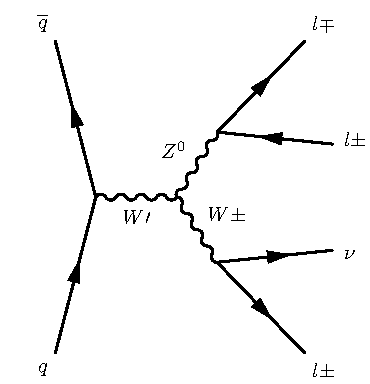
\includegraphics[width=0.4\textwidth]{fig/WprimeFeynmanDiagram.pdf}
  \caption{ Feynman Diagram of the decay for the
    electrically charged WZ resonance $W^{\prime}$}
  \label{fig:Wprime_FeynmanDiagram}
\end{figure}

In this analysis, we test a set of theoretical models based on a phenomenological
lagrangian that contains Heavy Vector Triplets (HVT): the HVT framework, which
generalizes a large number of models predicting Spin-1 resonances ~\cite{hvt2014}.
Using two benchmarks: A weakly coupled extended gauge symmetry (referred as model A) and a
strongly coupled composite higgs scenario (model B). Further theoretical treatment of these models
is provided by Refs. ~\cite{hvt2014,modelA1980,modelB2011}. Specifically, a search
for an electrically charged resonance $W^{\prime}$ is performed. This search focuses
on the $W^{\prime}$ fully leptonic decay:
$W^{\prime}\rightarrow WZ \rightarrow \ell\nu \ell\ell$ ($\ell = e$ or $\mu$).
Despite the low branching ratio of the leptonic decay, it offers low SM backgrounds and high
sensitivity in the low mass resonance range. In this channel, the SM $Z^{0}$
boson decays to a pair of same flavoured, opposite charged leptons and the
electrically charged $W^{\pm}$ decays to a lepton and a neutrino, see Feynman diagram
on figure \ref{fig:Wprime_FeynmanDiagram}. The neutrino $\nu$ escapes
undetected and therefore needs to be reconstructed from the missing transverse
energy in the Compact Muon Solenoid (CMS) detector.

Initial studies look for an enhancement of the Signal/Background ratio,
based on the kinematic variables to find regions in the phase-space sensitive
to the presence of the signal; these include studies on the performance of
the High Level Trigger, different options of lepton identification, isolation,
and other detector-specific requirements.

The accuracy of the MC simulations for the SM processes is then studied in a
dedicated signal-depleted control region of the phase space. A variety of
corrections on the MC samples are applied in order to account for the different
rates of efficiencies in the data reconstruction, particle identification, and
inefficiencies in the simulation of generated processes, as well as the
contribution from multiple proton-to-proton interactions occurring per bunch
crossing at the LHC accelerator.

The spectrum of the invariant mass for the diboson resonance candidates is
examined where a localized excess of events is expected if the resonance is
found, or otherwise, an agreement with the rates predicted by the standard model
within the statistical and systematic uncertainties will be found.
A fit to a background-only and background plus signal hypothesis is performed
through maximum likelihood estimation. Systematic uncertainties effects are
treated as nuisance parameters of the likelihood function.

The analysis is based on proton-proton collision data, with a center of mass
energy of $\sqrt{s}=13$ TeV collected by the CMS collaboration during the the
2016-2018 period, corresponding to an integrated luminosity of $L=137.2~fb^{-1}$.


\section{Data Samples}

The datasets used for the analysis presented in this note were collected using
the CMS detector during the period 2016-2018. Data was recorded at the
center-of-mass energy $\sqrt{s}=13~TeV$ and a total of $137.4~fb^{-1}$ was collected
and reconstructed with the 10.2.18 version of the CMS software. The standard
CMS selection of good runs and luminosity sections was applied
(see table \ref{tab:GoldenJson}).

The analysis makes use of datasets which combine several High Level Trigger
(HLT) paths. The datasets used are shown in table \ref{tab:Datasets}, each
dataset contains in the order of hundreds of millions events. As an event
may trigger different HLTs it may be stored in multiple datasets simultaneously.
In order to prevent double counting an index list is built containing unique
references to events based on their run and event number.

\begin{table}[h]
\centering
\caption{List of datasets used in the analysis.}
\begin{tabular}{|l|l|l|l|}
\hline
Year & Dataset & Run & Version \\ \hline
2016 & SingleMuon     & B           & ver2-v1 \\
     &                & C,D,E,F,G,H & v1      \\
     & SingleElectron & B           & ver2-v1 \\
     &                & C,D,E,F,G,H & v1      \\
     & SinglePhoton   & B           & ver2-v1 \\
     &                & C,D,E,F,G,H & v1      \\ \hline
2017 & SingleMuon     & B,C,D,E,F & v1 \\
     & SingleElectron & B,C,D,E,F & v1 \\
     & SinglePhoton   & B,C,D,E,F & v1 \\\hline
2018 & SingleMuon & A,B,C,D & v1 \\
     & EGamma     & A,B,C,D & v1 \\ \hline
\end{tabular}
\label{tab:Datasets}
\end{table}


\begin{table}[htbp]
  \footnotesize
  \topcaption{
    The golden JSON files
  }
  \centering
  \label{tab:gJSON}
  \begin{tabular}{ c l }
    \hline
    Year & File \\
    \hline
    2016 & Cert\_271036-284044\_13TeV\_ReReco\_07Aug2017\_Collisions16\_JSON.txt \\
    2017 & Cert\_294927-306462\_13TeV\_PromptReco\_Collisions17\_JSON.txt \\
    2018 & Cert\_314472-325175\_13TeV\_PromptReco\_Collisions18\_JSON.txt \\
    \hline
  \end{tabular}
  \label{tab:GoldenJson}
\end{table}

\subsection{Triggers}



\section{Montecarlo Samples}

The analysis uses a set of centrally produced Montecarlo (MC) \verb|NanoAODv6|
samples corresponding to the \verb|Summer16|, \verb|Fall17|, and \verb|Autumn18|
campaigns.


\subsection {Signal Samples}

Signal events for electrically charged diboson resonances in the $600~GeV$
to $4.5~TeV$ mass range under the theoretical assumptions of the HVT model
have been generated using Monte Carlo (MC) simulations with \verb|MadGraph5_aMC@NL| ~\cite{madgraph}
interfaced with Pythia 8 ~\cite{pythia} for showering and hadronization, and a
full detector response simulated with the \verb|Geant4| toolkit ~\cite{geant4}.
Physics objects are then reconstructed using the Particle-flow
algorithm ~\cite{particleflow}.

A complete list of the signal samples being used is shown in
table \ref{tab:SignalList}


\begin{sidewaystable}[htb]
\begin{center}
  \caption{Signal samples used in this analysis, their associated cross section
  times the branching ratio}
\footnotesize
\begin{tabular}{|l|l|l|l|}
\hline
Year & Sample & XSec Model A [pb] & XSec Model B [pb]\\ \hline
\hline
2016 & WprimeToWZToWlepZlep\_narrow\_M-600\_13TeV-madgraph  & 6.252E-2 & 0. \\
 &WprimeToWZToWlepZlep\_narrow\_M-800\_13TeV-madgraph  & 1.886E-2 & 1.02E-02\\
 &WprimeToWZToWlepZlep\_narrow\_M-1000\_13TeV-madgraph & 7.381E-3 & 6.81E-03\\
 &WprimeToWZToWlepZlep\_narrow\_M-1200\_13TeV-madgraph & 3.356E-3 & 3.75E-03\\
 &WprimeToWZToWlepZlep\_narrow\_M-1400\_13TeV-madgraph & 1.684E-3 & 2.08E-03\\
 &WprimeToWZToWlepZlep\_narrow\_M-1600\_13TeV-madgraph & 9.036E-4 & 1.19E-03\\
 &WprimeToWZToWlepZlep\_narrow\_M-1800\_13TeV-madgraph & 5.087E-4 & 6.97E-04\\
 &WprimeToWZToWlepZlep\_narrow\_M-2000\_13TeV-madgraph & 2.967E-4 & 4.18E-04\\
 &WprimeToWZToWlepZlep\_narrow\_M-2500\_13TeV-madgraph & 8.548E-5 & 1.25E-04\\
 &WprimeToWZToWlepZlep\_narrow\_M-3000\_13TeV-madgraph & 2.680E-5 & 4.02E-05\\
 &WprimeToWZToWlepZlep\_narrow\_M-3500\_13TeV-madgraph & 8.754E-6 & 1.33E-05\\
 &WprimeToWZToWlepZlep\_narrow\_M-4000\_13TeV-madgraph & 2.893E-6 & 4.53E-06\\
 &WprimeToWZToWlepZlep\_narrow\_M-4500\_13TeV-madgraph & 9.543E-7 & 1.49E-06\\
\hline
2017 & WprimeToWZToWlepZlep\_narrow\_M600\_13TeV-madgraph  & 6.252E-2 & 0. \\
 &WprimeToWZToWlepZlep\_narrow\_M800\_13TeV-madgraph  & 1.886E-2 & 1.02E-02\\
 &WprimeToWZToWlepZlep\_narrow\_M1000\_13TeV-madgraph & 7.381E-3 & 6.81E-03\\
 &WprimeToWZToWlepZlep\_narrow\_M1200\_13TeV-madgraph & 3.356E-3 & 3.75E-03\\
 &WprimeToWZToWlepZlep\_narrow\_M1400\_13TeV-madgraph & 1.684E-3 & 2.08E-03\\
 &WprimeToWZToWlepZlep\_narrow\_M1600\_13TeV-madgraph & 9.036E-4 & 1.19E-03\\
 &WprimeToWZToWlepZlep\_narrow\_M1800\_13TeV-madgraph & 5.087E-4 & 6.97E-04\\
 &WprimeToWZToWlepZlep\_narrow\_M2000\_13TeV-madgraph & 2.967E-4 & 4.18E-04\\
 &WprimeToWZToWlepZlep\_narrow\_M2500\_13TeV-madgraph & 8.548E-5 & 1.25E-04\\
 &WprimeToWZToWlepZlep\_narrow\_M3000\_13TeV-madgraph & 2.680E-5 & 4.02E-05\\
 &WprimeToWZToWlepZlep\_narrow\_M3500\_13TeV-madgraph & 8.754E-6 & 1.33E-05\\
 &WprimeToWZToWlepZlep\_narrow\_M4000\_13TeV-madgraph & 2.893E-6 & 4.53E-06\\
 &WprimeToWZToWlepZlep\_narrow\_M4500\_13TeV-madgraph & 9.543E-7 & 1.49E-06\\
\hline
2018 & WprimeToWZToWlepZlep\_narrow\_M600\_13TeV-madgraph  & 6.252E-2 & 0. \\
 &WprimeToWZToWlepZlep\_narrow\_M800\_13TeV-madgraph  & 1.886E-2 & 1.02E-02\\
 &WprimeToWZToWlepZlep\_narrow\_M1000\_13TeV-madgraph & 7.381E-3 & 6.81E-03\\
 &WprimeToWZToWlepZlep\_narrow\_M1200\_13TeV-madgraph & 3.356E-3 & 3.75E-03\\
 &WprimeToWZToWlepZlep\_narrow\_M1400\_13TeV-madgraph & 1.684E-3 & 2.08E-03\\
 &WprimeToWZToWlepZlep\_narrow\_M1600\_13TeV-madgraph & 9.036E-4 & 1.19E-03\\
 &WprimeToWZToWlepZlep\_narrow\_M1800\_13TeV-madgraph & 5.087E-4 & 6.97E-04\\
 &WprimeToWZToWlepZlep\_narrow\_M2000\_13TeV-madgraph & 2.967E-4 & 4.18E-04\\
 &WprimeToWZToWlepZlep\_narrow\_M2500\_13TeV-madgraph & 8.548E-5 & 1.25E-04\\
 &WprimeToWZToWlepZlep\_narrow\_M3000\_13TeV-madgraph & 2.680E-5 & 4.02E-05\\
 &WprimeToWZToWlepZlep\_narrow\_M3500\_13TeV-madgraph & 8.754E-6 & 1.33E-05\\
 &WprimeToWZToWlepZlep\_narrow\_M4000\_13TeV-madgraph & 2.893E-6 & 4.53E-06\\
 &WprimeToWZToWlepZlep\_narrow\_M4500\_13TeV-madgraph & 9.543E-7 & 1.49E-06\\
\hline
\end{tabular}
\label{tab:SignalList}
\end{center}
\end{sidewaystable}

\subsection{Background Samples}

Background processes have been generated using MadGraph, Pythia and Powheg
generators. These backgrounds include irreducible processes which produce the
same final state as the signal and also reducible processes which produce
different physics, but lead to similar signals in the detector. The backgrounds
or dominiated by the production of electroweak heavy vector boson pairs (WZ), but
also include ZZ production where one of the leptons is either outside the detector
acceptans or mis-reconstructed. Other backgrounds such as Z+Jets, $t\bar{t}$,
$Z\gamma$, are included as they may contain mis-identified lepton candidates
coming from jets or photons.

The full list of background samples, including their dataset name and cross
section, are presented in tables \ref{tab:BkgList2016} (2016),
\ref{tab:BkgList2017}(2017), \ref{tab:BkgList2018} (2018).

\begin{sidewaystable}[htb]
\begin{center}
  \caption{List of background samples for the Summer16 campaign, their
    associated cross section times branching ratio and the plotting group
    in which each one is included.}
\footnotesize
\begin{tabular}{|l|l|l|}
\hline
Background  & Sample & XSec [pb] \\ \hline
\hline $WZ\rightarrow\ell\nu\ell\ell$
&WZTo3LNu\_mllmin01\_13TeV-powheg-pythia8  & 6.217e+01 \\
\hline $ZZ\rightarrow4\ell$
&ZZTo4L\_13TeV\_powheg\_pythia8 & 1.256 \\
\hline $t\bar{t}$
&TTJets\_DiLept\_TuneCUETP8M1\_13TeV-madgraphMLM-pythia8 & 5.675e1 \\
\hline $Z\gamma\rightarrow\ell\ell\gamma$
&ZGTo2LG\_TuneCUETP8M1\_13TeV-amcatnloFXFX-pythia8 & 1.24e2 \\
\hline Z+Jets
& DYJetsToLL\_M-50\_HT-100to200\_TuneCUETP8M1\_13TeV-madgraphMLM-pythia8   & 1.475e2 \\
& DYJetsToLL\_M-50\_HT-200to400\_TuneCUETP8M1\_13TeV-madgraphMLM-pythia8   & 4.104e1 \\
& DYJetsToLL\_M-50\_HT-400to600\_TuneCUETP8M1\_13TeV-madgraphMLM-pythia8   & 5.676   \\
& DYJetsToLL\_M-50\_HT-600to800\_TuneCUETP8M1\_13TeV-madgraphMLM-pythia8   & 1.36    \\
& DYJetsToLL\_M-50\_HT-800to1200\_TuneCUETP8M1\_13TeV-madgraphMLM-pythia8  & 6.218e-1\\
& DYJetsToLL\_M-50\_HT-1200to2500\_TuneCUETP8M1\_13TeV-madgraphMLM-pythia8 & 1.512e-1\\
& DYJetsToLL\_M-50\_HT-2500toInf\_TuneCUETP8M1\_13TeV-madgraphMLM-pythia8  & 3.659e-3\\
\hline TTV
&TTWJetsToLNu\_TuneCUETP8M1\_13TeV-amcatnloFXFX-madspin-pythia8 & 2.007e-1 \\
&TTZToLL\_M-1to10\_TuneCUETP8M1\_13TeV-madgraphMLM-pythia8      & 0.283    \\
&ttZJets\_13TeV\_madgraphMLM-pythia8                            & 6.559e-1 \\
\hline VVV
&WWW\_4F\_TuneCUETP8M1\_13TeV-amcatnlo-pythia8 & 2.086e-1 \\
&WWZ\_TuneCUETP8M1\_13TeV-amcatnlo-pythia8     & 1.651e-1 \\
&WZZ\_TuneCUETP8M1\_13TeV-amcatnlo-pythia8     & 5.565e-2 \\
&ZZZ\_TuneCUETP8M1\_13TeV-amcatnlo-pythia8     & 1.398e-2 \\
\hline $gg\rightarrow4\ell\ell$
&GluGluToContinToZZTo2e2mu\_13TeV\_MCFM701\_pythia8 & 5.423e-3 \\
&GluGluToContinToZZTo4e\_13TeV\_MCFM701\_pythia8    & 2.703e-3 \\
&GluGluToContinToZZTo4mu\_13TeV\_MCFM701\_pythia8   & 2.703e-3 \\
&GluGluToContinToZZTo4tau\_13TeV\_MCFM701\_pythia8  & 2.703e-3 \\
\hline Single Top
&ST\_s-channel\_4f\_leptonDecays\_13TeV-amcatnlo-pythia8\_TuneCUETP8M1                      & 3.365   \\
&ST\_t-channel\_antitop\_4f\_inclusiveDecays\_13TeV-powhegV2-madspin-pythia8\_TuneCUETP8M1  & 80.95   \\
&ST\_t-channel\_top\_4f\_inclusiveDecays\_13TeV-powhegV2-madspin-pythia8\_TuneCUETP8M1      & 136.02  \\
&ST\_tW\_antitop\_5f\_inclusiveDecays\_13TeV-powheg-pythia8\_TuneCUETP8M1                   & 3.806e1 \\
&ST\_tW\_top\_5f\_inclusiveDecays\_13TeV-powheg-pythia8\_TuneCUETP8M1                       & 3.809e1 \\
\hline
\end{tabular}
\label{tab:BkgList2016}
\end{center}
\end{sidewaystable}




\begin{sidewaystable}[htb]
\begin{center}
  \caption{List of background samples for the Fall17 campaign, their
    associated cross section times branching ratio and the plotting group
    in which each one is included.}
\footnotesize
\begin{tabular}{|l|l|l|}
\hline
Background  & Sample & XSec [pb] \\ \hline
\hline $WZ\rightarrow\ell\nu\ell\ell$
&WZTo3LNu\_mllmin01\_NNPDF31\_TuneCP5\_13TeV\_powheg\_pythia8  & 6.217e+01 \\
\hline $ZZ\rightarrow4\ell$
&ZZTo4L\_13TeV\_powheg\_pythia8 & 1.256 \\
\hline $t\bar{t}$
&TTJets\_DiLept\_TuneCP5\_13TeV-madgraphMLM-pythia8 & 5.420e+1 \\
\hline $Z\gamma\rightarrow\ell\ell\gamma$
&ZGToLLG\_01J\_5f\_TuneCP5\_13TeV-amcatnloFXFX-pythia8 & 5.547e1 \\
\hline Z+Jets
& DYJetsToLL\_M-50\_HT-100to200\_TuneCP5\_13TeV-madgraphMLM-pythia8   & 1.475e2 \\
& DYJetsToLL\_M-50\_HT-200to400\_TuneCP5\_13TeV-madgraphMLM-pythia8   & 4.104e1 \\
& DYJetsToLL\_M-50\_HT-400to600\_TuneCP5\_13TeV-madgraphMLM-pythia8   & 5.676   \\
& DYJetsToLL\_M-50\_HT-600to800\_TuneCP5\_13TeV-madgraphMLM-pythia8   & 1.36    \\
& DYJetsToLL\_M-50\_HT-800to1200\_TuneCP5\_13TeV-madgraphMLM-pythia8  & 6.218e-1\\
& DYJetsToLL\_M-50\_HT-1200to2500\_TuneCP5\_13TeV-madgraphMLM-pythia8 & 1.512e-1\\
& DYJetsToLL\_M-50\_HT-2500toInf\_TuneCP5\_13TeV-madgraphMLM-pythia8  & 3.659e-3\\
\hline TTV
&TTZToLL\_M-1to10\_TuneCP5\_13TeV-amcatnlo-pythia8      & 5.324e-2    \\
&ttZJets\_TuneCP5\_13TeV\_madgraphMLM\_pythia8          &  5.420e-1   \\
&TTWJetsToLNu\_TuneCUETP8M1\_13TeV-amcatnloFXFX-madspin-pythia8 & 2.144e-1 \\
\hline VVV
&WWW\_4F\_TuneCP5\_13TeV-amcatnlo-pythia8 & 2.086e-1 \\
&WWZ\_4F\_TuneCP5\_13TeV-amcatnlo-pythia8 & 1.651e-1 \\
&WZZ\_TuneCP5\_13TeV-amcatnlo-pythia8     & 5.565e-2 \\
&ZZZ\_TuneCP5\_13TeV-amcatnlo-pythia8     & 1.398e-2 \\
\hline $gg\rightarrow4\ell\ell$
&GluGluToContinToZZTo2e2mu\_13TeV\_TuneCP5\_MCFM701\_pythia8 & 5.423e-3 \\
&GluGluToContinToZZTo4e\_13TeV\_TuneCP5\_MCFM701\_pythia8    & 2.703e-3 \\
&GluGluToContinToZZTo4mu\_13TeV\_TuneCP5\_MCFM701\_pythia8   & 2.703e-3 \\
&GluGluToContinToZZTo4tau\_13TeV\_TuneCP5\_MCFM701\_pythia8  & 2.703e-3 \\
\hline Single Top
&ST\_s-channel\_4f\_leptonDecays\_TuneCP5\_13TeV-amcatnlo-pythia8                       & 3.740   \\
&ST\_t-channel\_antitop\_4f\_inclusiveDecays\_TuneCP5\_13TeV\-powhegV2-madspin-pythia8  & 6.791e+1   \\
&ST\_t-channel\_top\_4f\_inclusiveDecays\_TuneCP5\_13TeV-powhegV2-madspin-pythia8     & 1.133e+2 \\
&ST\_tW\_antitop\_5f\_inclusiveDecays\_TuneCP5\_13TeV-powheg-pythia8                  & 3.497e+1 \\
&ST\_tW\_top\_5f\_inclusiveDecays\_TuneCP5\_13TeV-powheg-pythia8                      & 3.491e+1 \\
\hline
\end{tabular}
\label{tab:BkgList2017}
\end{center}
\end{sidewaystable}


\begin{sidewaystable}[htb]
\begin{center}
  \caption{List of background samples for the Autumn18 campaign, their
    associated cross section times branching ratio and the plotting group
    in which each one is included.}
\footnotesize
\begin{tabular}{|l|l|l|}
\hline
Background  & Sample & XSec [pb] \\ \hline
\hline $WZ\rightarrow\ell\nu\ell\ell$
&WZTo3LNu\_mllmin01\_NNPDF31\_TuneCP5\_13TeV\_powheg\_pythia8  & 6.217e+01 \\
\hline $ZZ\rightarrow4\ell$
&ZZTo4L\_TuneCP5\_13TeV-amcatnloFXFX-pythia8 & 1.373\\
\hline $t\bar{t}$
&TTJets\_DiLept\_TuneCP5\_13TeV-madgraphMLM-pythia8 & 5.434e+1 \\
\hline $Z\gamma\rightarrow\ell\ell\gamma$
&ZGToLLG\_01J\_5f\_TuneCP5\_13TeV-amcatnloFXFX-pythia8 & 5.548e1 \\
\hline Z+Jets
& DYJetsToLL\_M-50\_HT-100to200\_TuneCP5\_PSweights\_13TeV-madgraphMLM-pythia8   & 1.608e2 \\
& DYJetsToLL\_M-50\_HT-200to400\_TuneCP5\_PSweights\_13TeV-madgraphMLM-pythia8   & 4.864e1 \\
& DYJetsToLL\_M-50\_HT-400to600\_TuneCP5\_PSweights\_13TeV-madgraphMLM-pythia8   & 6.982 \\
& DYJetsToLL\_M-50\_HT-600to800\_TuneCP5\_PSweights\_13TeV-madgraphMLM-pythia8   & 1.756 \\
& DYJetsToLL\_M-50\_HT-800to1200\_TuneCP5\_PSweights\_13TeV-madgraphMLM-pythia8  & 8.096e-1\\
& DYJetsToLL\_M-50\_HT-1200to2500\_TuneCP5\_PSweights\_13TeV-madgraphMLM-pythia8 & 1.931e-1\\
& DYJetsToLL\_M-50\_HT-2500toInf\_TuneCP5\_PSweights\_13TeV-madgraphMLM-pythia8  & 3.513e-3\\
\hline TTV
&TTWJetsToLNu\_TuneCUETP8M1\_13TeV-amcatnloFXFX-madspin-pythia8 & 2.181e-1 \\
&TTZToLL\_M-1to10\_TuneCP5\_13TeV-amcatnlo-pythia8      & 5.324e-2 \\
&ttZJets\_TuneCP5\_13TeV\_madgraphMLM\_pythia8          & 5.924e-1 \\
\hline VVV
&WWW\_4F\_TuneCP5\_13TeV-amcatnlo-pythia8 & 2.154e-1 \\
&WWZ\_4F\_TuneCP5\_13TeV-amcatnlo-pythia8 & 1.676e-1 \\
&WZZ\_TuneCP5\_13TeV-amcatnlo-pythia8     & 5.701e-2 \\
&ZZZ\_TuneCP5\_13TeV-amcatnlo-pythia8     & 1.473e-2 \\
\hline $gg\rightarrow4\ell\ell$
&GluGluToContinToZZTo2e2mu\_13TeV\_TuneCP5\_MCFM701\_pythia8 & 5.423e-3 \\
&GluGluToContinToZZTo4e\_13TeV\_TuneCP5\_MCFM701\_pythia8    & 2.703e-3 \\
&GluGluToContinToZZTo4mu\_13TeV\_TuneCP5\_MCFM701\_pythia8   & 2.703e-3 \\
&GluGluToContinToZZTo4tau\_13TeV\_TuneCP5\_MCFM701\_pythia8  & 2.703e-3 \\
\hline Single Top
&ST\_s-channel\_4f\_leptonDecays\_TuneCP5\_13TeV-amcatnlo-pythia8                       & 3.740 \\
&ST\_t-channel\_antitop\_5f\_inclusiveDecays\_TuneCP5\_13TeV\-powhegV2-madspin-pythia8  & 3.497e+1 \\
&ST\_tW\_antitop\_5f\_inclusiveDecays\_TuneCP5\_13TeV-powheg-pythia8                  & 3.497e+1 \\
&ST\_tW\_top\_5f\_inclusiveDecays\_TuneCP5\_13TeV-powheg-pythia8                      & 3.491e+1 \\
\hline
\end{tabular}
\label{tab:BkgList2018}
\end{center}
\end{sidewaystable}



\section{Object definitions and Event selection}

\subsection{Event cleanup and vertex selection}

\begin{figure}[tph]
  \centering
  \subfigure[2016]{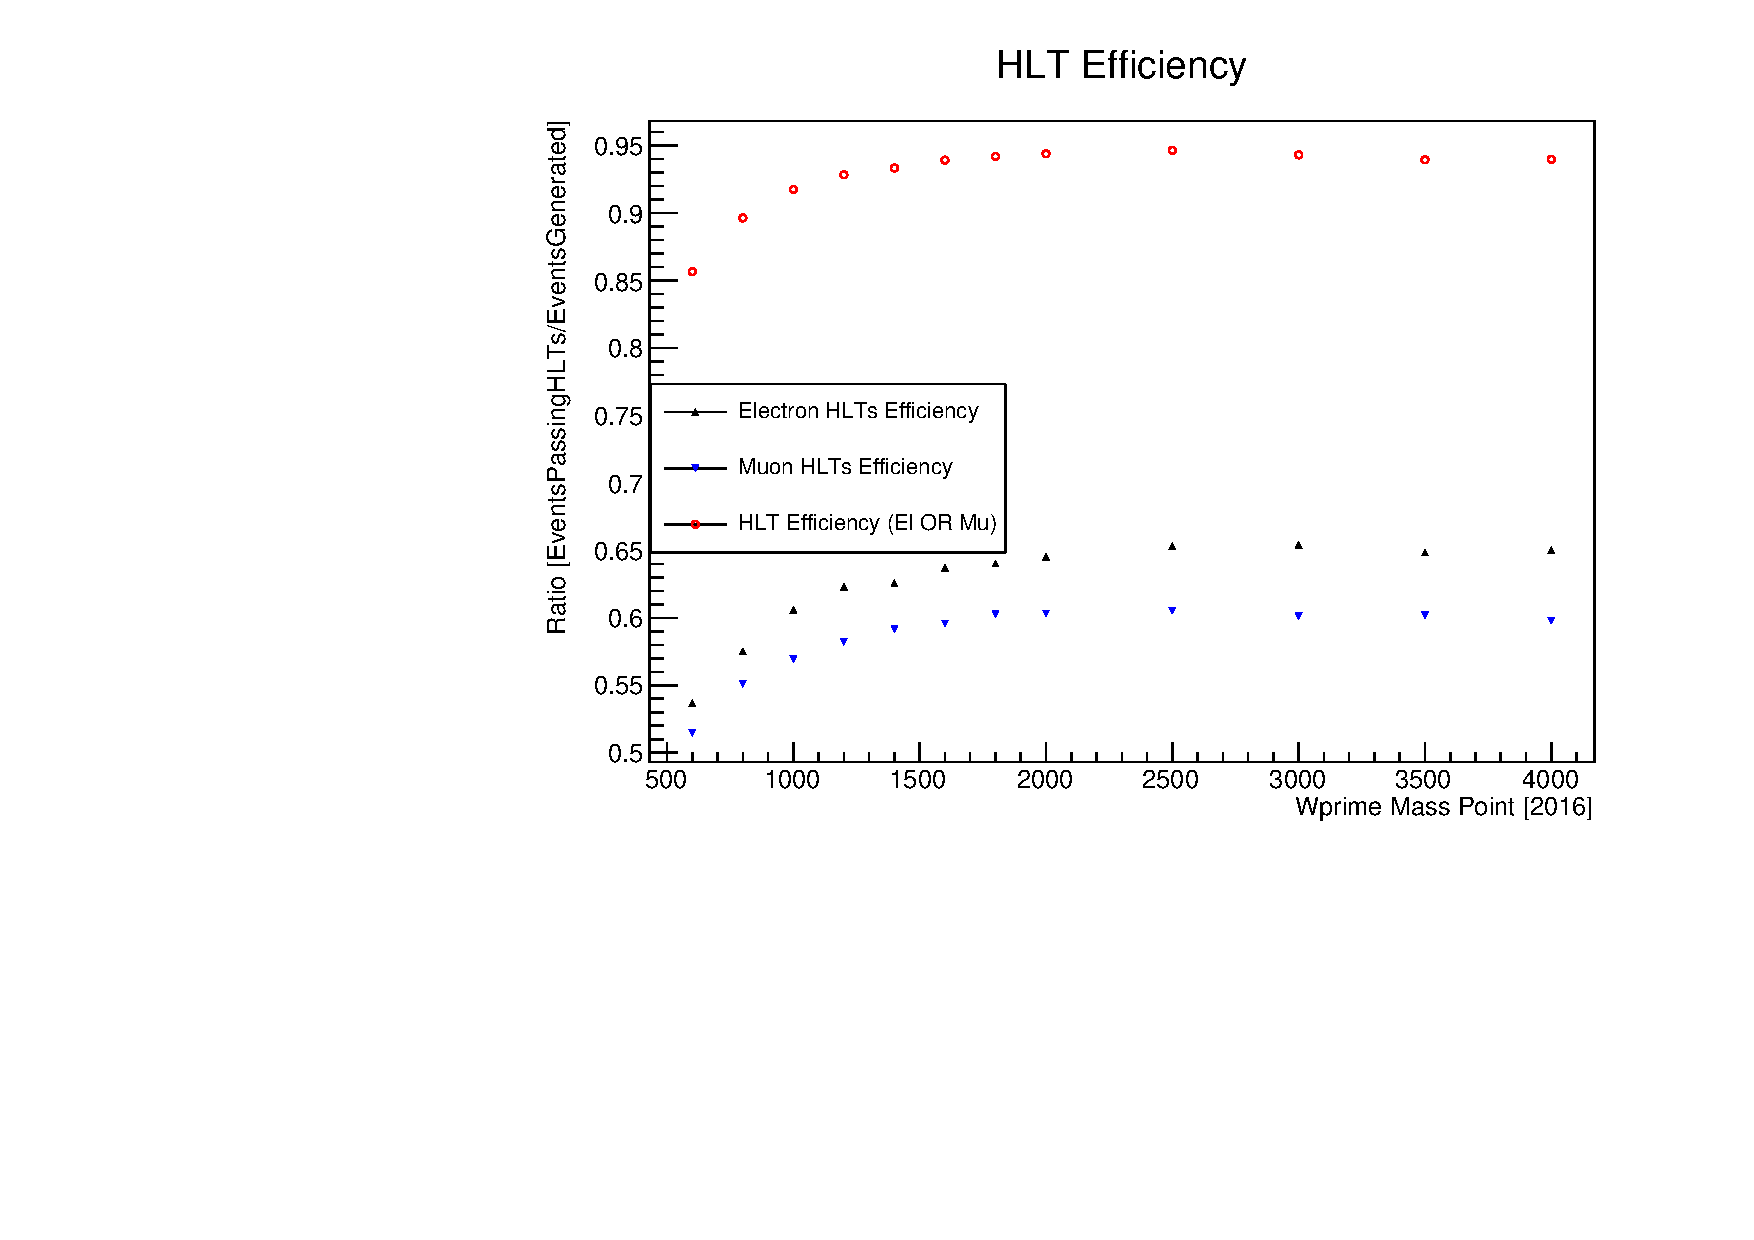
\includegraphics[width=.5\textwidth]{fig/2016_SignalTriggerEfficiency.pdf}}
  \subfigure[2017]{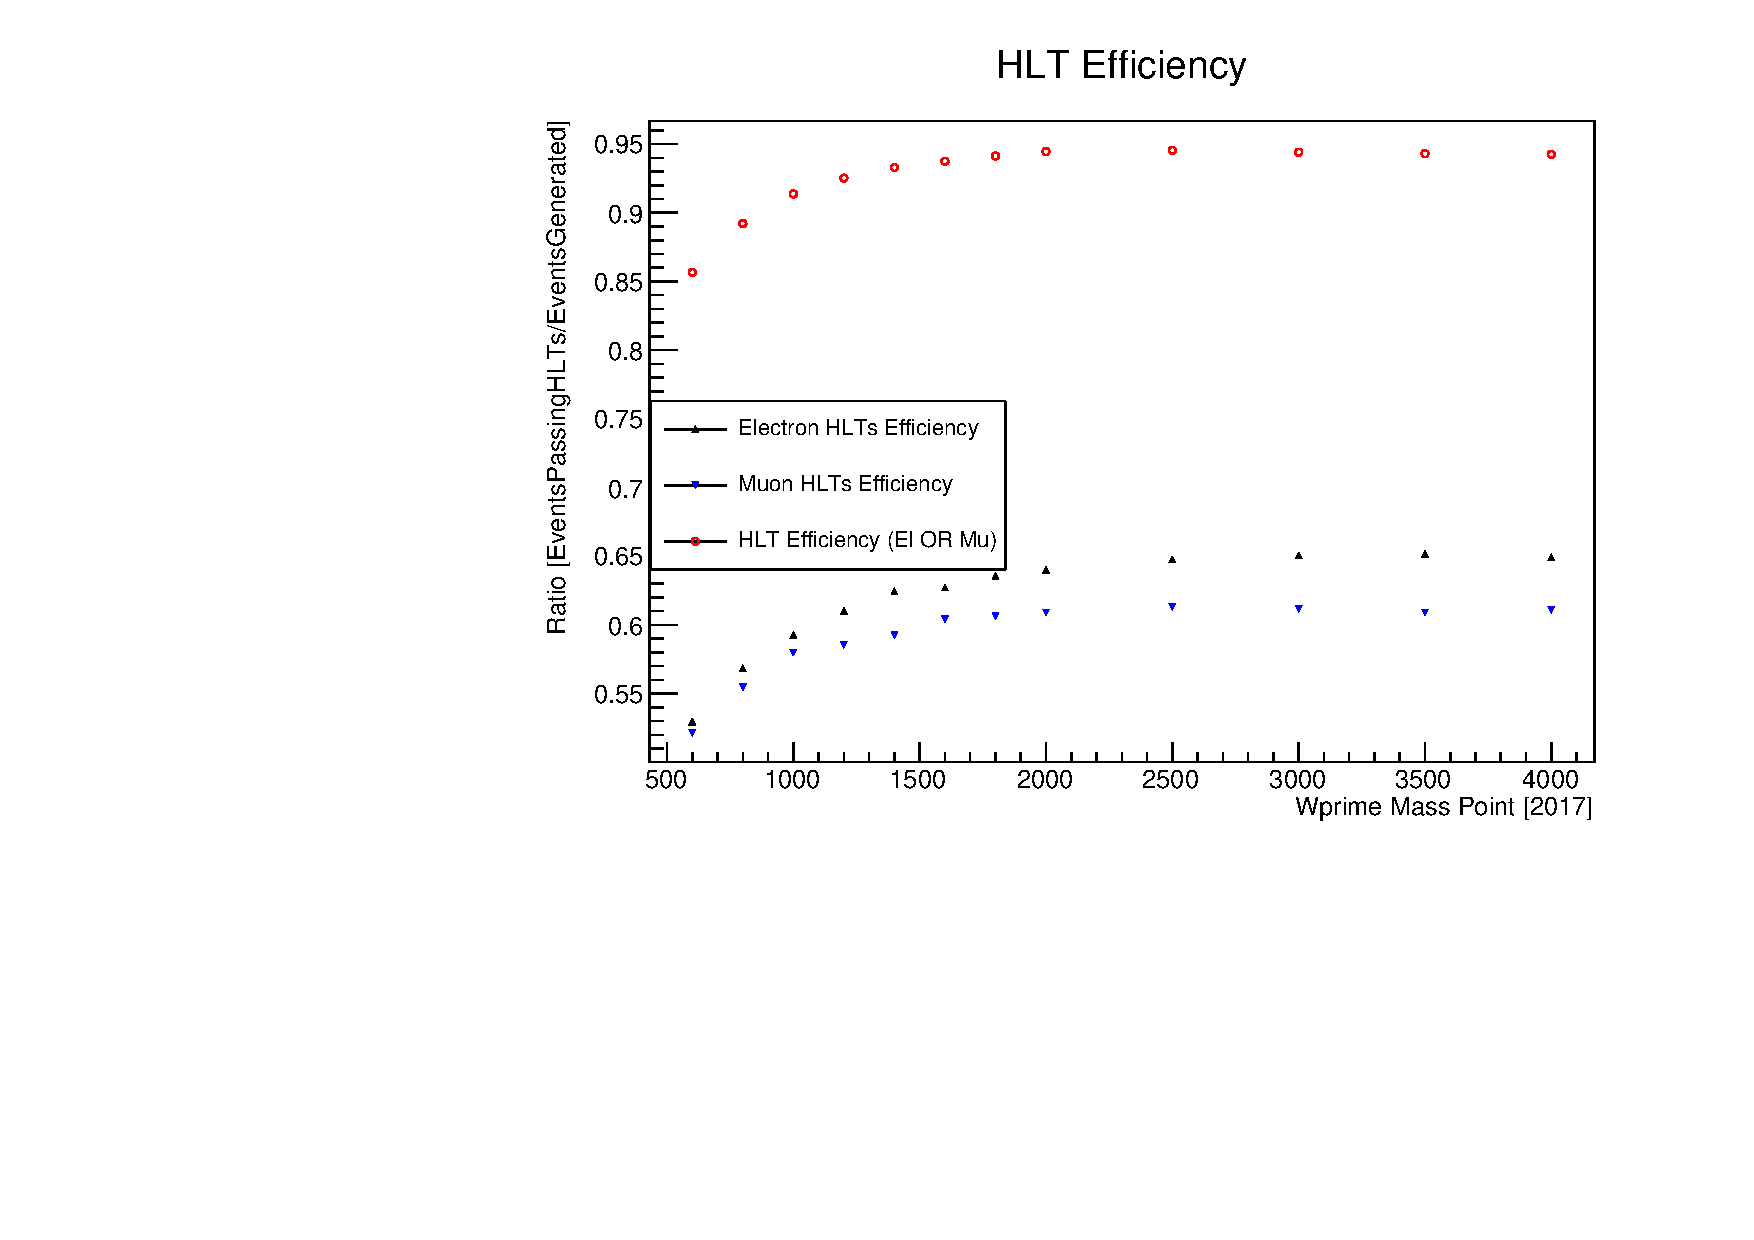
\includegraphics[width=.5\textwidth]{fig/2017_SignalTriggerEfficiency.pdf}}
  \vfil
  \subfigure[2018]{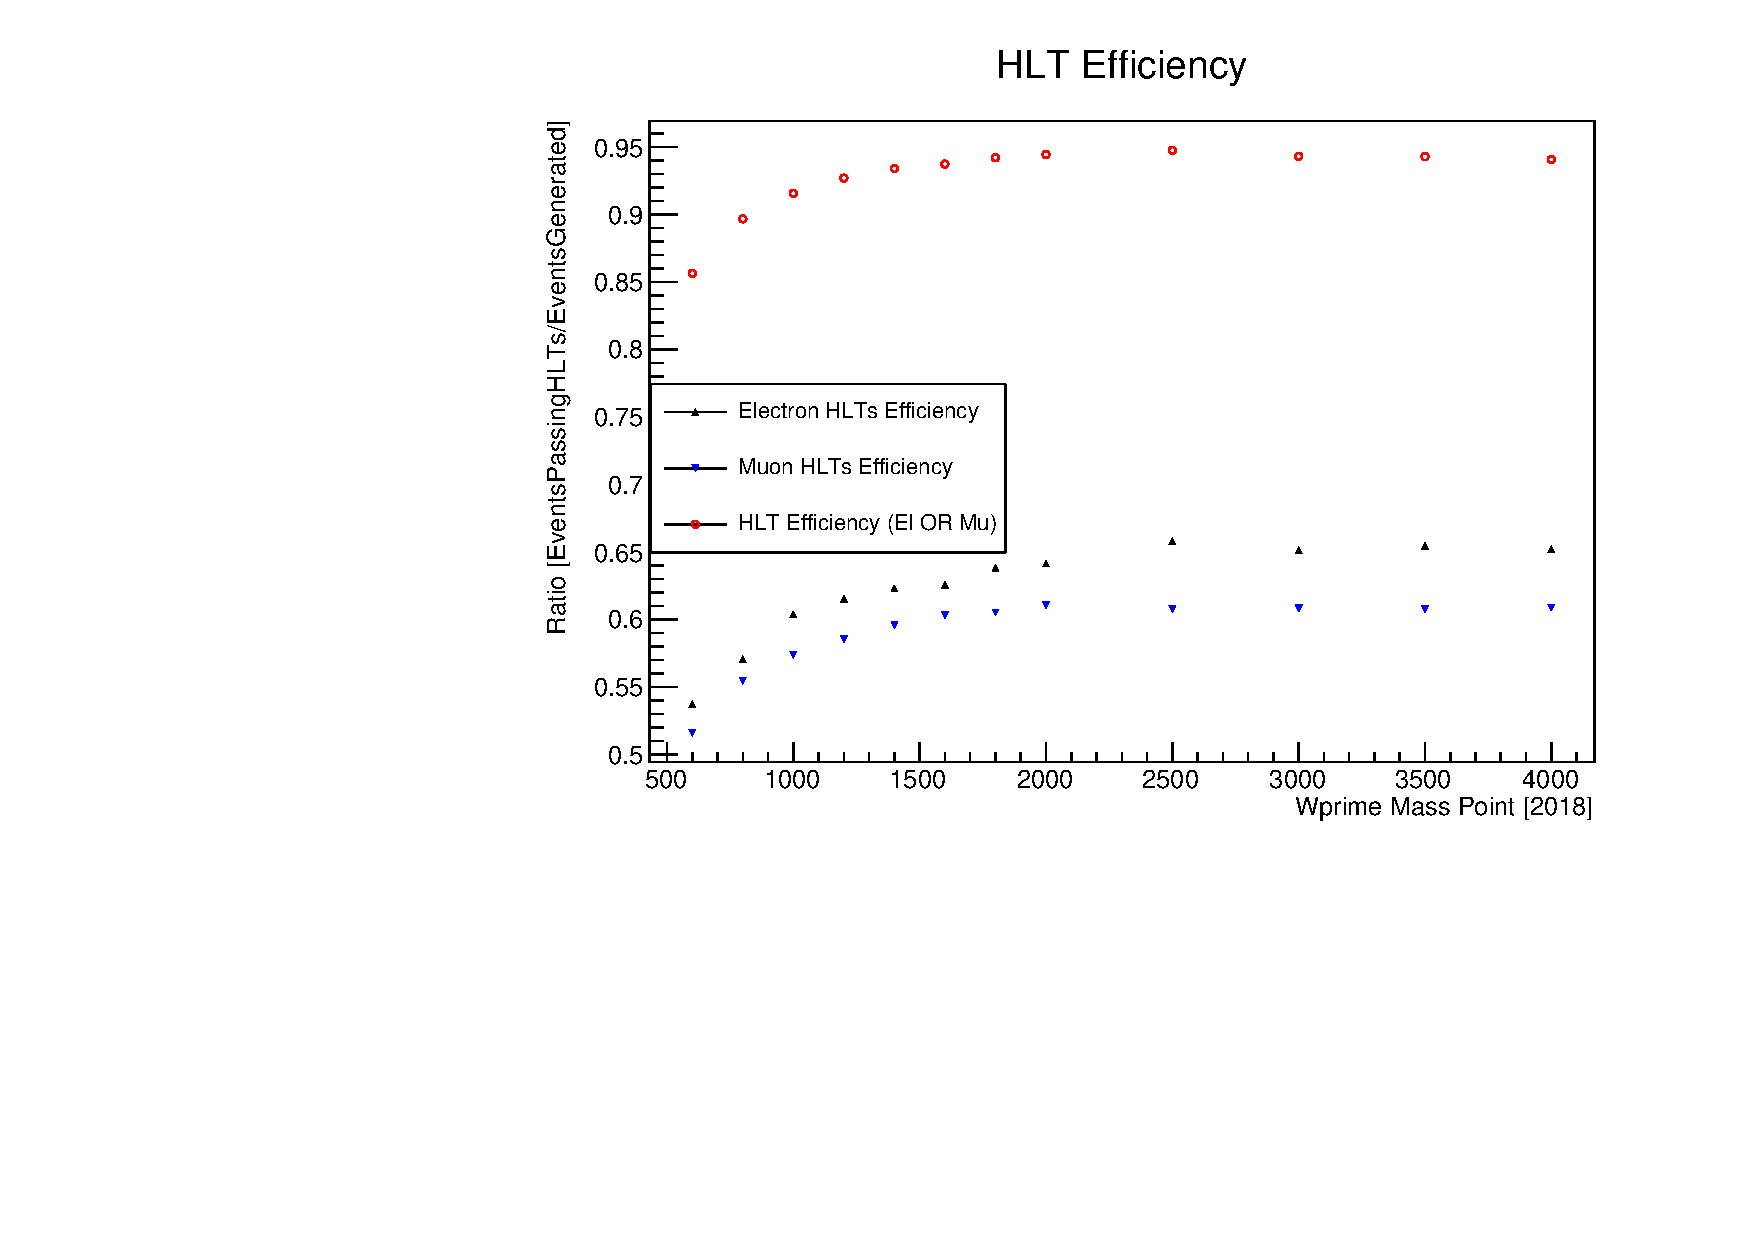
\includegraphics[width=.5\textwidth]{fig/2018_SignalTriggerEfficiency.pdf}}
  \caption{Signal efficiency for individual and combined High Level Triggers for Run II. Electron and
    Muon HLT paths are shown in Table \ref{tab:HLTDatasets}.
  }
  \label{fig:hltSignalEfficiency}
\end{figure}


Events with at least one primary vertex passing an OR combination
of the HLTs shown on table \ref{tab:HLTDatasets}, and containing at least three
preselected leptons (number of muons plus number of electrons) are selected
provided that its missing energy $E_T^{Miss}$ is greater than $40~GeV$.
Due to the presence of multiple leptonic flavors in the final state, each event
is required to pass either the Muon or Electron triggers based on the high-Pt
recommendations from the POG. The HLT efficiency was found to be higher
than 85\% as shown in Figure \ref{fig:hltSignalEfficiency}.

In addition, the following flags are required for the event:

\begin{itemize}
  \item \verb|Flag_goodVertices|
  \item \verb|Flag_globalSuperTightHalo2016Filter|
  \item \verb|Flag_HBHENoiseFilter|
  \item \verb|Flag_HBHENoiseIsoFilter|
  \item \verb|Flag_EcalDeadCellTriggerPrimitiveFilter|
  \item \verb|Flag_BadPFMuonFilter|
\end{itemize}

One additional flag is required for the year 2017, 2018:

\begin{itemize}
\item \verb|Flag_ecalBadCalibFilterV2|
\end{itemize}

\subsection{Lepton Selection}

\subsection{Electron Selection}

\verb|Electron| collection in \verb|NanoAOD|

Electrons are reconstructed from hits in the different
layers of the tracker and energy deposits in the scintillating crystalls
across the $\eta-\phi$ plane in the Electromagnetic Calorimeter.

The electron's sign charge can be identified by its signature in the tracker
due to the presence of the strong magnetic field in the CMS detector.

Electrons in this analysis are required to be within the ECAL fiducial
region i.e $\abs{\eta}<2.5$ excluding the transition region betwen the
barrel and the endcaps $1.4442<\abs{\eta}<1.5660$.

\begin{figure}[tph]
  \centering
  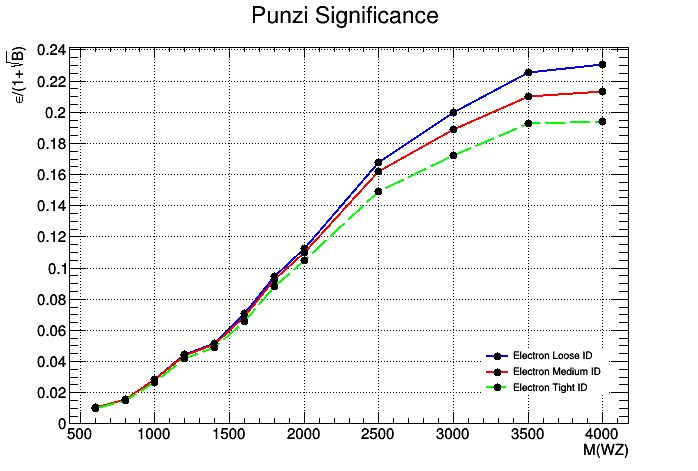
\includegraphics[width=0.6\textwidth]{fig/LeptonIDStudies/ElectronIDPunzi.png}
  \caption{Punzi significance for the different Electron's cut-based IDs for the
    electron decay $Z\rightarrow e+e$. The cut-based loose ID shows high efficiency
    specially at high masses where the distance in the $\eta-\phi$ plane is
    expected to be small.}
  \label{fig:PunziElectronIDs}
\end{figure}

Electron identification is based on a cut based ID as defined by the
EGamma POG. Depending on the channel, this requirement
may ask for \emph{loose} or \emph{tight} electrons, the former with an
average efficiency of approximately 95\% and 70\% for
the latter ~\cite{EGammaPOG_el}: channels with a $Z\rightarrow e+e$
decay ($eee\nu$ and $ee\mu\nu$) require two loose
electrons due to its high efficiency, specially at high resonant mass where
the electrons are expected to be highly collimated (see Figure \ref{fig:PunziElectronIDs}).
The electron corresponding to the $W\rightarrow e\nu$ decay is required to pass
the cut-based tight ID.

We reproduce the High Level Trigger transverse momentum requirements by
applying a cut on the corresponding $p_T$ threshold on all
preselected electrons:
2016 ($27~GeV$), 2017 ($35~GeV$), and 2018 ($32~GeV$).

\subsection{Muon Selection}

\verb|Muon| collection in \verb|NanoAOD|

The muon objects in this analysis can be divided into two categories:
Tracker and Global highPt muons ~\cite{MuonPOG}. Tracker highPt muons are
reconstructed from hits in the tracker matched with hits in the first
muon station, while global highPt muons leave trace beyond the first
layer of the muon subsystem.

Muons are required to be within the pseudorapidity range $\abs{\eta}<2.4$ and
to have a minimum transverse momentum of $P_t=20$. Additionally the leading muon
is required to have a transverse momentum $P_t>52~GeV$ in line with
the trigger plateau.

\begin{figure}[tph]
  \centering
  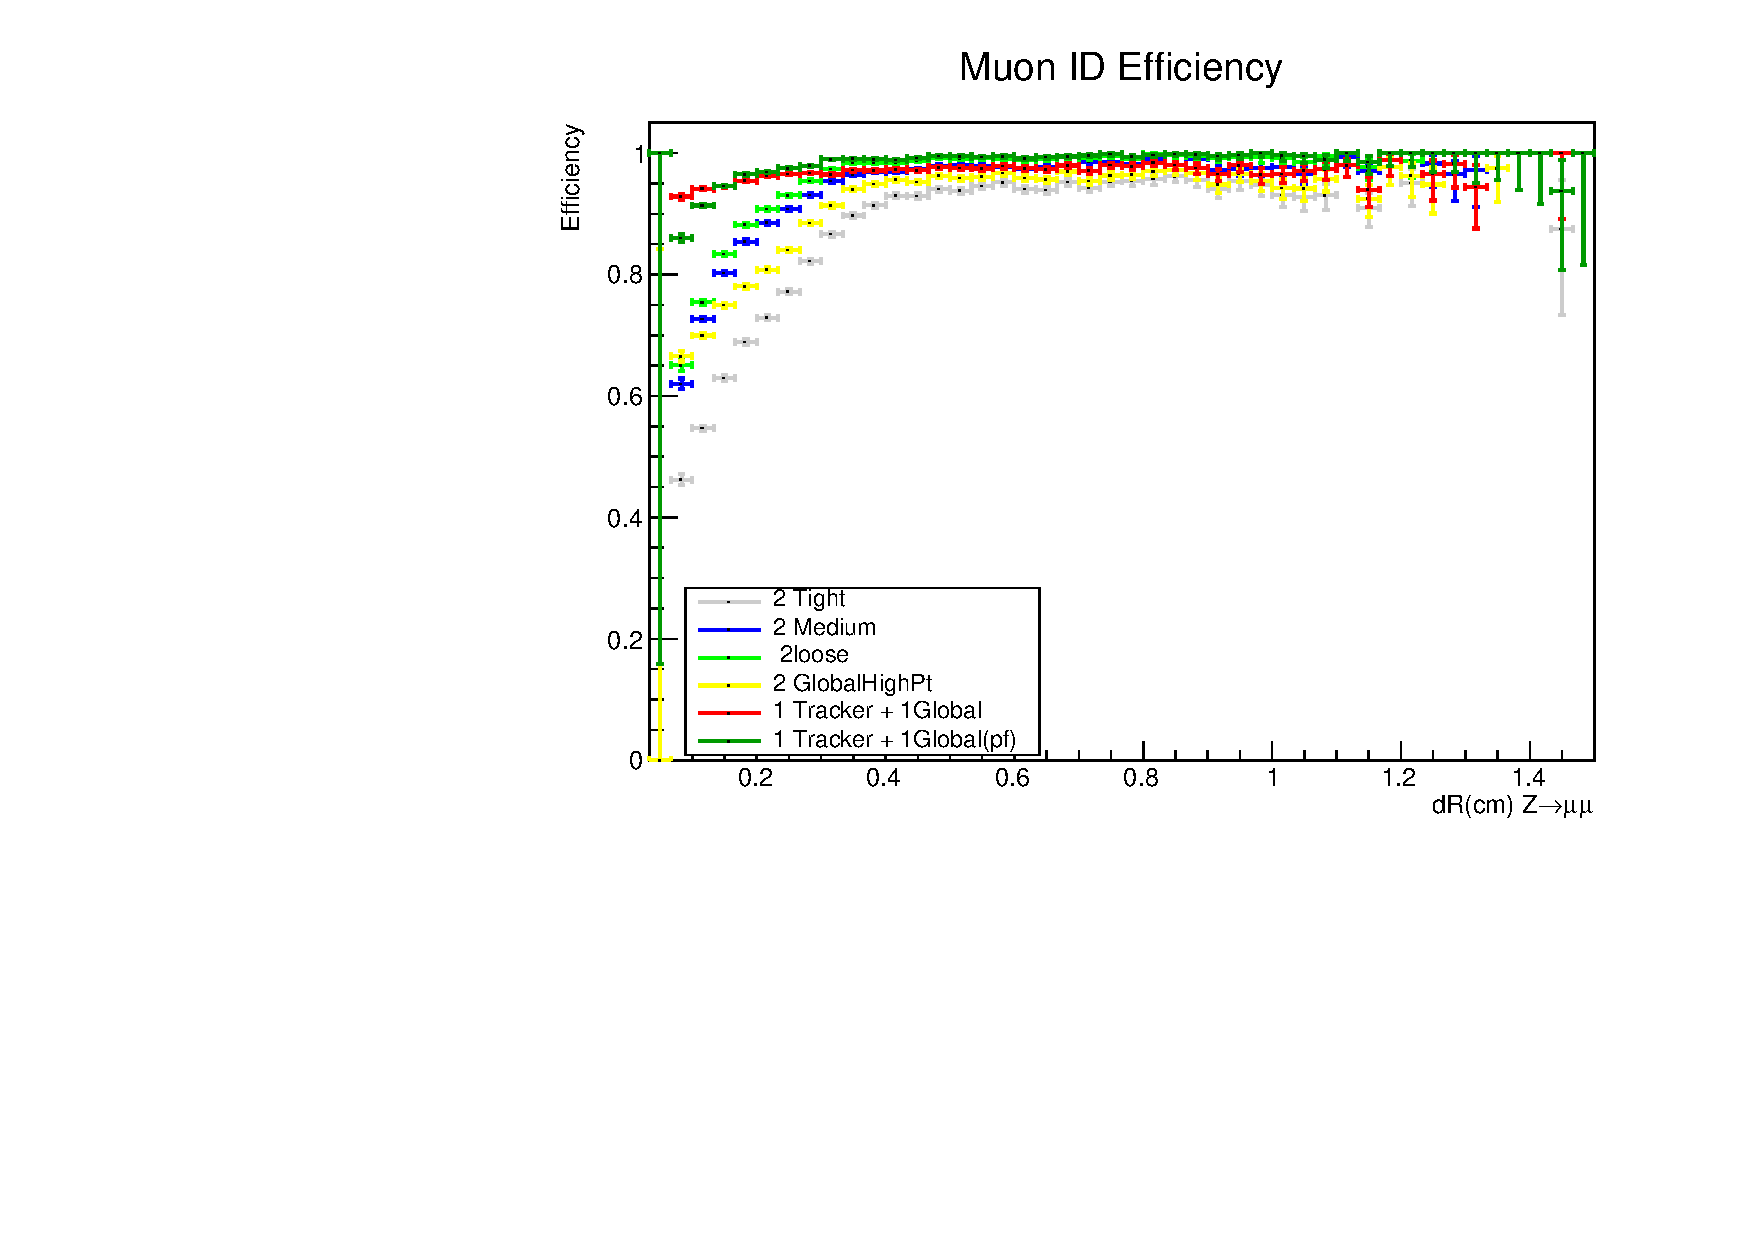
\includegraphics[width=0.6\textwidth]{fig/LeptonIDStudies/MuonIDEfficiency.pdf}
  \caption{Signal Efficiency for different Muon ID combinations for the product of
    the decay $Z\rightarrow\mu+\mu$. The less efficient combination is requiring
    the Muon pair to be a cut-based Tight ID pair, increasing efficiency towards less
    strict cut-based requirements (Loose and Medium ID). The most efficient combination in
    the signal reconstruction is the combination of one global-highPt ID Muon
    with another muon that can be either a tracker or global-HighPt ID.}
  \label{fig:MuonIDEfficiency}
\end{figure}

For events portraying a $Z\rightarrow\mu+\mu$ decay a stricter cut is applied on the
leading muon $P_{t}>70~GeV$. The muon pair is required to be a composite of a
cut-based global highPt ID muon and either a tracker or global highPt ID muon
that is simultaneously a particle-flow candidate. This combination of highPt
muons shows the highest efficiency, see Figure \ref{fig:MuonIDEfficiency}.
%%% Add reference to B2G-19-006 %%%

Events with a pair of muons with an impact parameter $ip3d>0.01~cm$ are
discarded in order to increase background rejection.



\subsection{Lepton Misidentification}

\begin{figure}[tph]
  \centering
  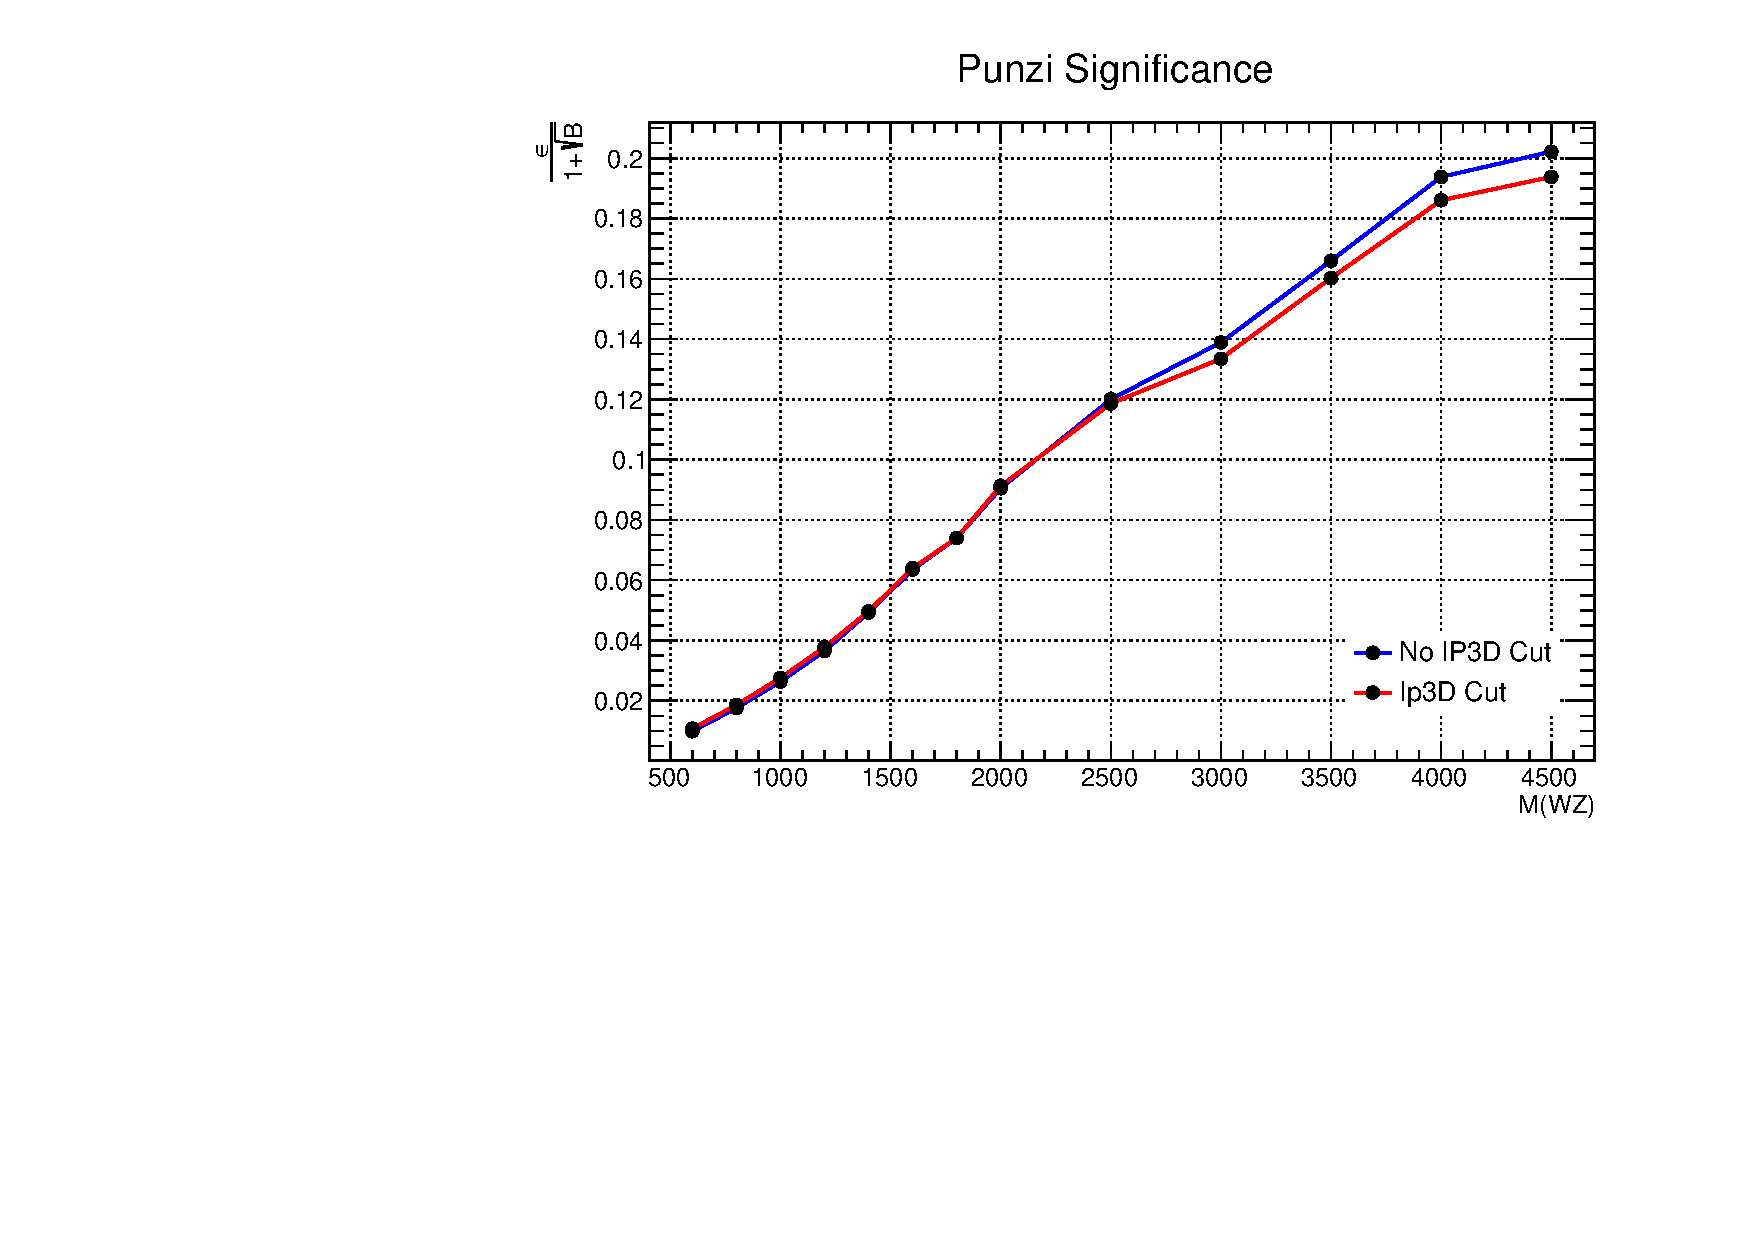
\includegraphics[width=0.6\textwidth]{fig/PunziTest_Ip3DCut.pdf}
  \caption{Punzi significance as a function of the mass resonce prior to and after implementing
    the cut on the impact parameter in order to reduce the number of non-prompt
    muons}
  \label{fig:Punzi_Ip3DCut}
\end{figure}

The nature of the reconstruction process may lead to some objects being
wrongly identified. A dedicated study was performed in order to evaluate
the effects on misreconstructed objects on the counting experiment.
Misreconstructed leptons are also commonly refered as fake leptons. It
is assumed that if the number of MC generated electrons (muons) match
the number of reconstructed electrons (muons) there are no misreconstructed
objects. A fake lepton is a lepton that is non-prompt that didn't arise from
a $\tau$ lepton or from a heavy flavour decay (HFD). Figure %%Missing Figure %%%
shows how the Drell-Yan and $t\bar{t}$ processes are suceptible to present
reconstructed non-prompt muons. To account for this, we impose a cut on the
3D impact parameter $ip3D<0.01~cm$, figure %%Missing Figure %%%
shows the effect of the cut on reducing the number of non-prompt muons.
The Punzi significance of the impact parameter requirement as a function
of the WZ resonance mass is shown in figure \ref{fig:Punzi_Ip3DCut}. %%% expand %%%


\begin{figure}[tph]
  \centering
  \subfigure[Lepton origin classification prior to constraining the impact parameter]
            {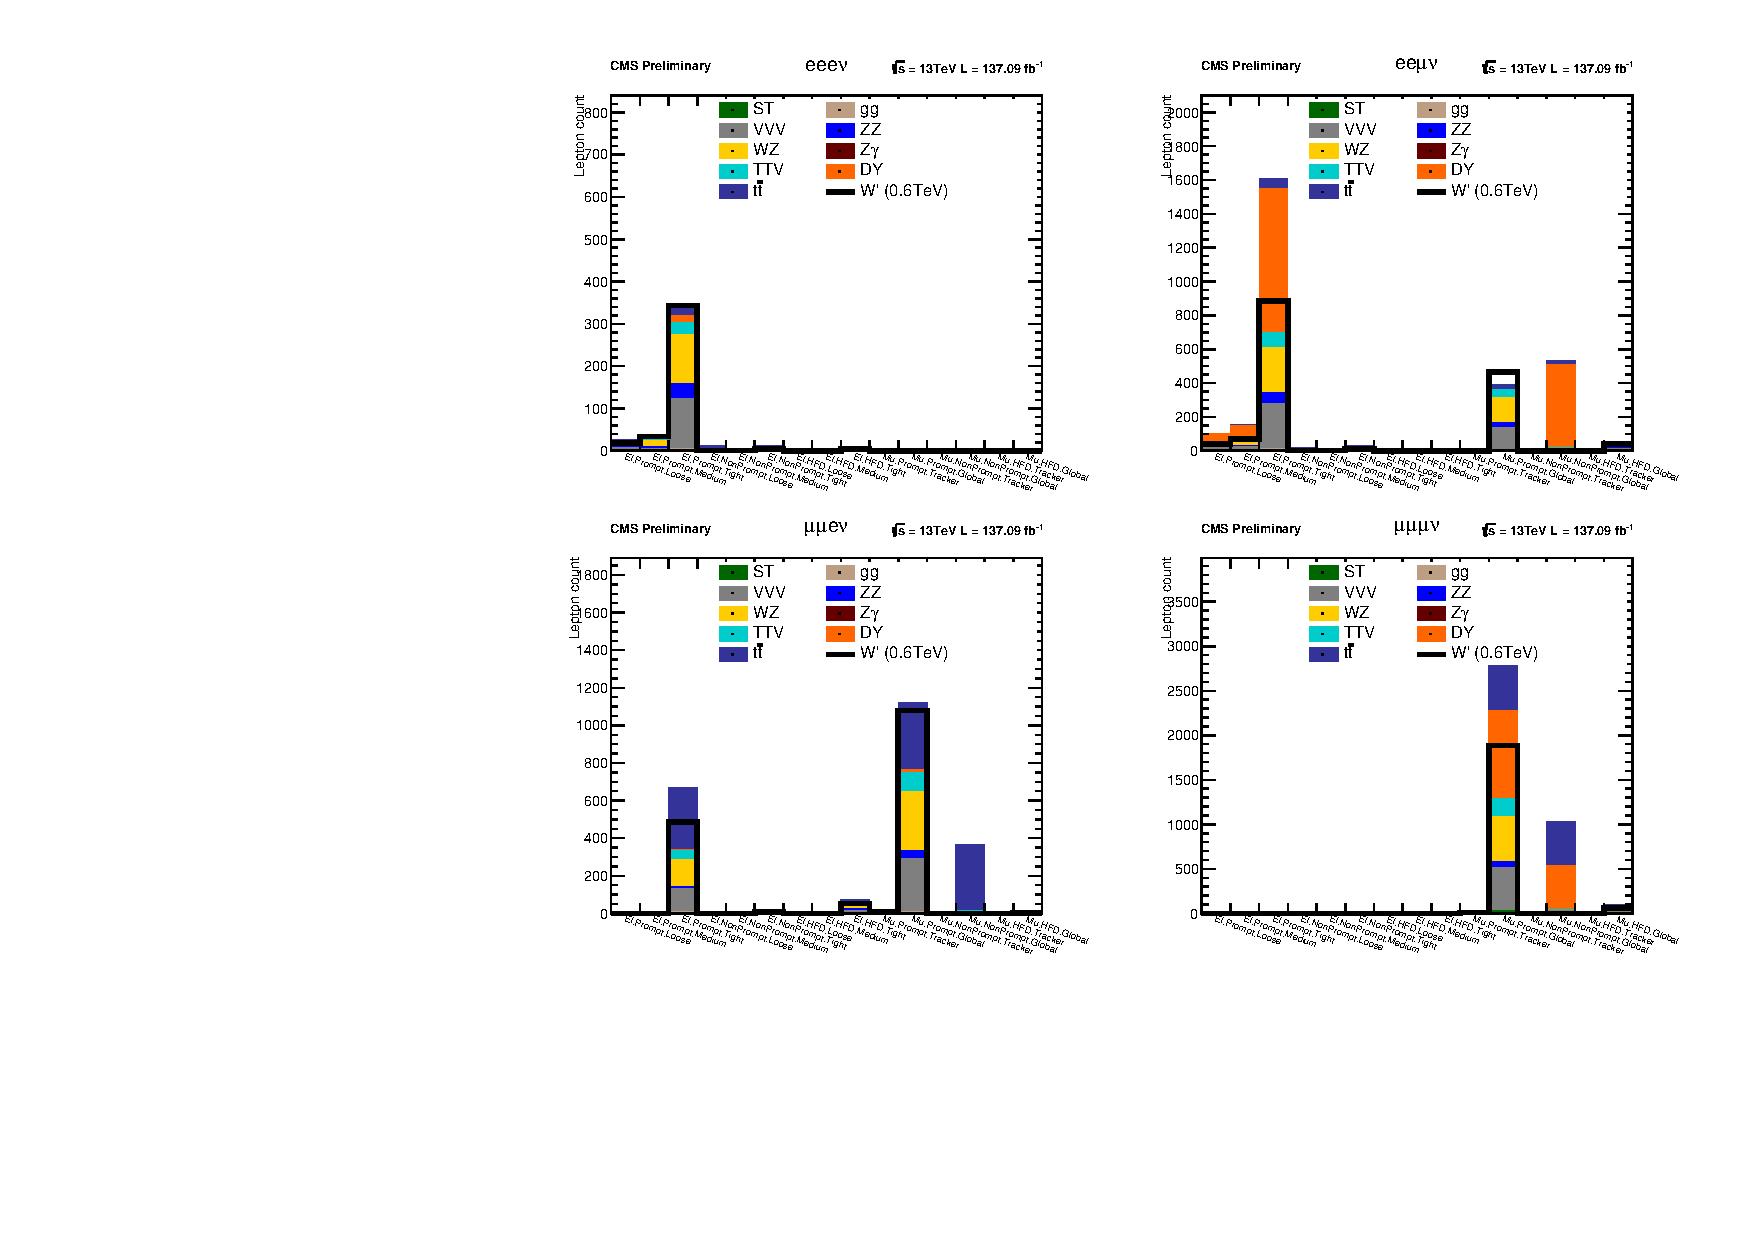
\includegraphics[width=.8\textwidth]{fig/Run2/NoIp3DCut_HFakeString_SR1_A_RuRun2_M600.pdf}}
  \vfil
  \subfigure[Lepton origin classification after constraining the impact parameter $ip3D<0.01~cm$]
            {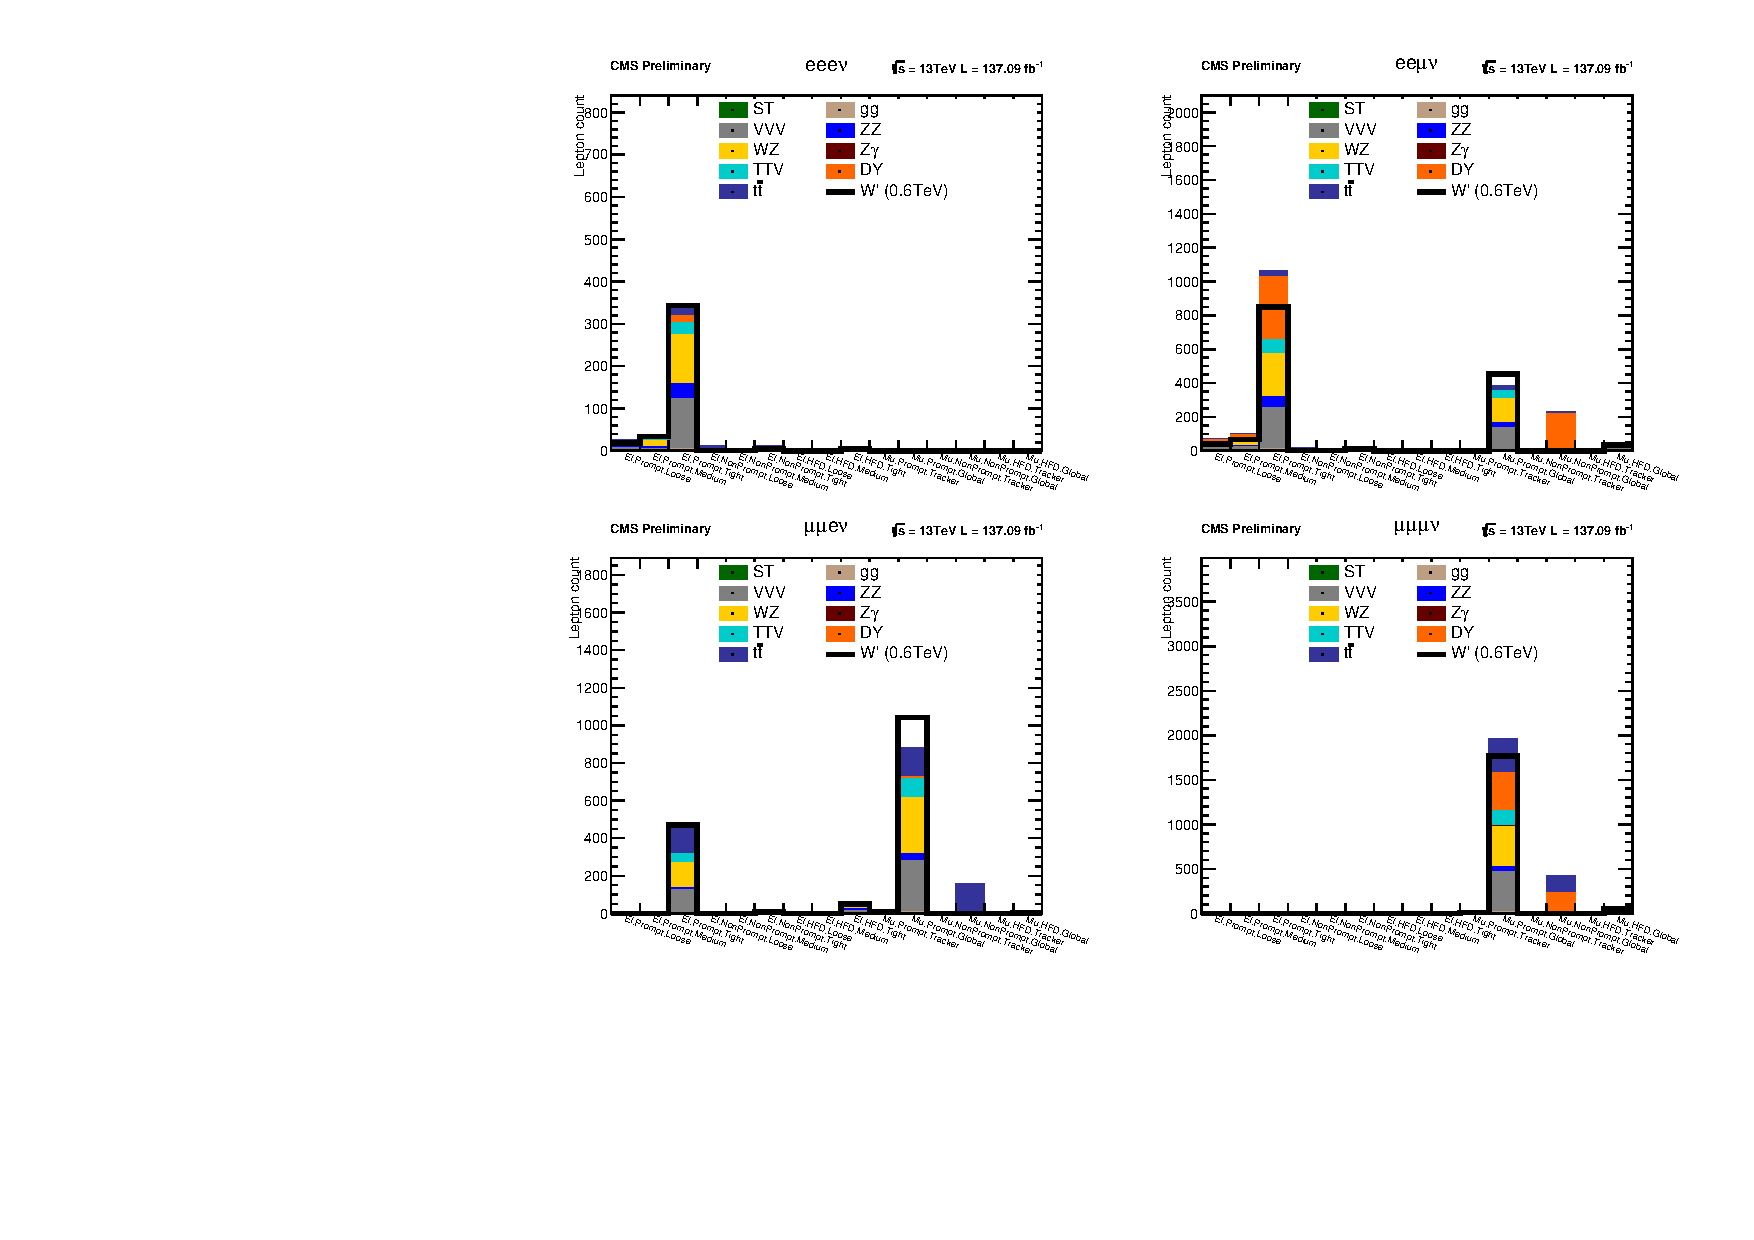
\includegraphics[width=.8\textwidth]{fig/Run2/Rebining_HFakeString_SR1_A_RuRun2_M600.pdf}}
  \caption{Lepton origin classification according to simulation prior and after applying
    an impact parameter requirement $ip3D<0.01~cm$. Each lepton is considered individually
    when filling the histogram. The main contribution to non-prompt leptons come
    from Muons in Drell-Yan and $t\bar{t}$ events.
  }
  \label{fig:HFakeString}
\end{figure}


\subsection{Missing Transverse Energy}

The missing transverse energy $E_T$ is reconstructed with the particle flow
algorithm ~\cite{particleflow} and events are required to have at least a
missing transverse energy of $E_T^{miss}=40~GeV$.

\subsection{Z Candidate}

Two same flavored, opposite charged leptons are required to reconstruct a Z
candidate. If more than one pair is found, the one with reconstructed mass
closer to the nominal mass $M_z=91.1876~GeV$ is chosen. The pair's mass
is required to fall in the Z mass window $70~GeV < M_Z < 111~GeV$. In favor of an
increase in the signal efficiency the opposite charged requirement is dropped
for the $eee\nu$ category.

If the Z candidate is formed from a muon pair with a leading (subleading) muon with
a transverse momentum of at least $P_t=70 GeV$ ($P_t=10GeV$). One of the
muons is required to pass two additional requirements: being a global high-Pt muon and a
particle-flow candidate. In the case of electrons, the requirement is to pass the
selection criteria of the cut-based \emph{loose} ID and a transverse momentum of
matching the trigger plateau.

The event is rejected from the signal region if the distance in the $\eta-\phi$
plane for the two leptons product of the decay of the Z is less than $1.5$.

\subsection{W Candidate}

The $W$ candidate is reconstructed from the remaining lepton and the missing energy
of the event $E_T^{miss}$. The remaining lepton is required to be either a cut based \emph{tight}
ID electron or a global High-Pt muon with a transverse momentum
of at least $Pt>52~GeV$.

The neutrino from the $W \rightarrow l\nu$ decay escapes undetected,
and therefore the following assumptions are made in order to perform a kinematic
reconstruction of the $W$ candidate: there are no additional sources of missing
energy, and consequently $E_{Pt}^{miss}$ is considered the transverse momentum
corresponding to the undetected neutrino. The longitudinal momentum $P_z$ can be
recovered by imposing the $M_W=80.379~GeV $ nominal mass and assuming
a massless neutrino $M_\nu = 0.$

As $\eta$ is unknown for the missing transverse energy, the neutrino 4-vector is
not well defined. However, by assuming the mass of $W$ the longitudinal component
of the neutrino is reduced to a quadratic equation:

\[
P_{Z}^{\nu} = \frac{P_{Z}^{l}({M_{W}^{2}-{M_{t}^{W}}^2+2P_{t}^{l}{P_{t}^{\nu}}}) \pm P^{l}\sqrt{(M_{W}^{2}-{M_{t}^{W}}^2)((M_{W}^{2}-{M_{t}^{W}}^2)+4P_{t}^{l}P_{t}^{\nu})}}{{2P_{t}^{l}}^{2}}
\]

Where the transverse mass $M_{t}^{W}$ is defined
as ${M_{t}^{W}}=\sqrt{2P_{t}^{l}P_{t}^{\nu}(1-cos\phi_{l\nu})}$.
Due to detector resolution effects and systematic uncertainties on the
reconstruction of missing transverse energy, the transverse mass may
exceed the mass of the $W$ boson $M_W$ and the
longitudinal component of the momentum would remain undefined, in these cases
we set the transverse mass equal to the nominal value $M_{t}^{W}=M_W$.

The less energetic of the solutions gives the correct value ~70\% of the time
according to simulation [AN].
When no real solutions are available ($W_{mt}$ > $Wm$), the invariant
mass is set to the reconstructed transverse mass and we are left with two real
identical solutions.

\subsection{WZ Candidate}

The $W^{\prime}$ is reconstructed from the $W$ and $Z$ candidates.
Events are rejected if the sum of the leptonic masses are less than $120~GeV$ and
if the sum of the transverse momentum $L_{t}<110~GeV$, where $L_{t}$ is defined
as:

\[
L_{t} = \sum_{n=1}^{3} Pt_{ln}
\]

Events are splitted in four channels depending on the leptonic flavour of the
diboson decay:

\begin{description}
\item[$\bullet$ $eee$] three electrons and missing transverse energy are found, two of the
  electrons correspond to the decay of the $Z$ boson and the remaining electron corresponds
  to the decay of the $W$ boson. $Z\rightarrow e^{+}e^{-} W\rightarrow e+\nu$
  The three electrons are expected to leave hits on the
  tracker subsystem with low curvature due to their high transverse momentum and
  energy depositions are expected in the electromagnetic calorimeter
  The signature left on the CMS detector is shown on figure \ref{fig:Fireworks_eeev}.
\item[$\bullet$ $ee\mu$] two electrons, one muon and missing transverse energy are found,
  the two electrons correspond to the decay of the $Z$ boson and the muon corresponds to the
  decay of the $W$ boson. $Z\rightarrow e^{+}e^{-} W\rightarrow \mu+\nu$ The two electrons are
  expected to leave hits on the tracker subsystem with low curvature and energy
  depositions are expected in the electromagnetic calorimeter while the muon leaves
  hits in the tracker and muon subsytem. The signature left on the CMS
  detector is shown on figure \ref{fig:Fireworks_eemuv}.
\item[$\bullet$ $\mu\mu e$] two muons, one electron and missing transverse energy are found,
  the two muons correspond to the decay of the $Z$ boson and the electron corresponds to the
  decay of the $W$ boson. $Z\rightarrow \mu^{+}\mu^{-} W\rightarrow e+\nu$ The two
  muons leave hits on the tracker and muon subsystems with negligible curvature due
  to its high transverse momentum while the electron is expected to leave hits in
  the tracker and energy deposition in the electromagnetica calorimeter.
  The signature left on the CMS detector is shown on figure \ref{fig:Fireworks_mumuev}.
\item[$\bullet$ $\mu\mu\mu$] three muons and missing transverse energy are found, the muon pair
  correspond to the decay of the $Z$ boson and the remianing muon corresponds
  to the decay of the $W$ boson. $Z\rightarrow \mu^{+}\mu^{-} W\rightarrow \mu+\nu$.
  The three muons are expected to leave hits on the tracker subsystem and muon chambers
  with low curvature due to their high transverse momenta. The signature
  left on the CMS detector is shown on figure \ref{fig:Fireworks_eemuv}.
\end{description}

\begin{figure}
  \centering
  \subfigure[Projection on the $\rho-\phi$ plane. \label{fig:A_RhoPhi}]{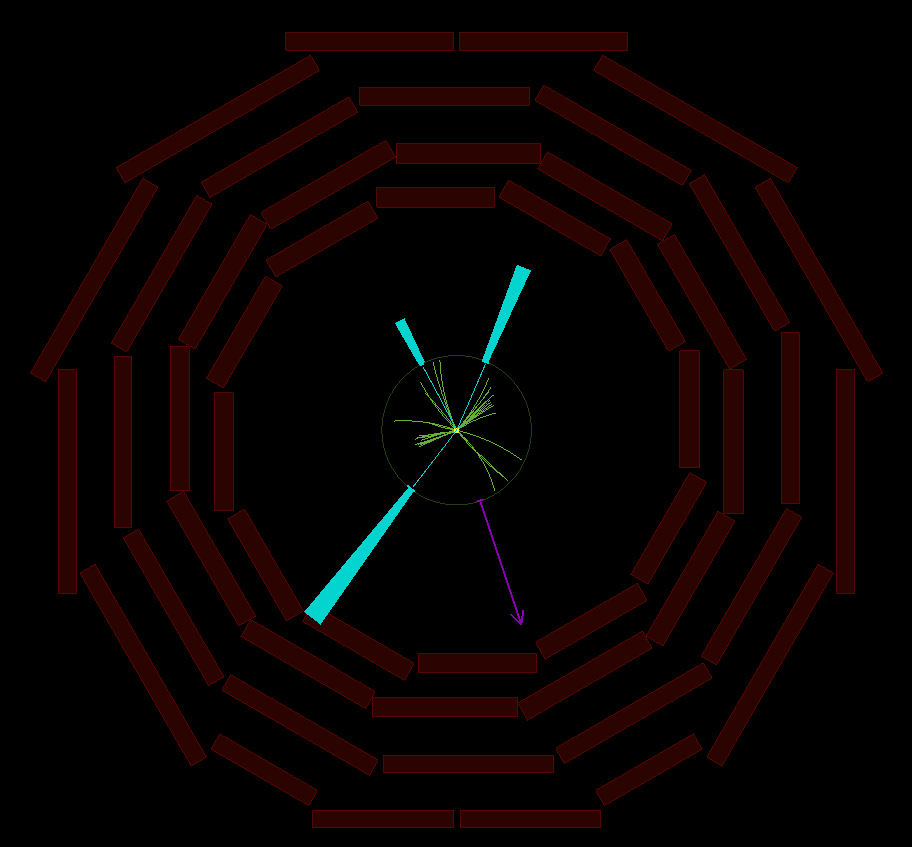
\includegraphics[width=0.8\linewidth]{fig/Fireworks/A_RhoPhi.png}}
  \vfil
  \subfigure[Projection on the $\rho-z$ plane\label{fig:A_RhoZ}]{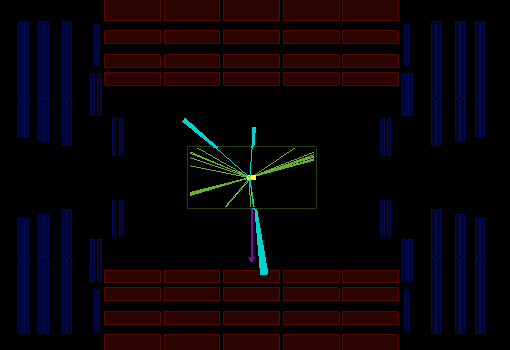
\includegraphics[width=0.40\linewidth]{fig/Fireworks/A_RhoZ.png}}
  \subfigure[3D view\label{fig:A_Rho3D}]{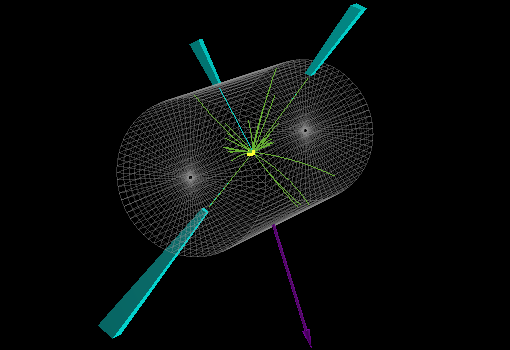
\includegraphics[width=0.40\linewidth]{fig/Fireworks/A_3D.png}}
  \caption{Example of the signature left on the detector by a signal-like event
    for the $eee\nu$ channel. This event was taken on July 13th 2018. Run: $319579$,
    Lumiblock: $2957$, Event: $4487890911$. The reconstructed primary vertex is shown in yellow.
    Depositions on the electromagnetic calorimeter and tracks left by the three electrons
    are shown in cyan, their area is proportional to the amount of energy deposited,
    the negligible curvature
    shown by their tracks is a reflection of their high transverse momentum. 
    The amount of missing transverse energy is proportional to the length of the purple arrow. Low momentum
    tracks for particle-flow candidates in the inner tracker are shown in green for
    reference, these PF candidates are filtered by the preselection. }
  \label{fig:Fireworks_eeev}
\end{figure}


\begin{figure}
  \centering
  \subfigure[Projection on the $\rho-\phi$ plane. \label{fig:B_RhoPhi}]{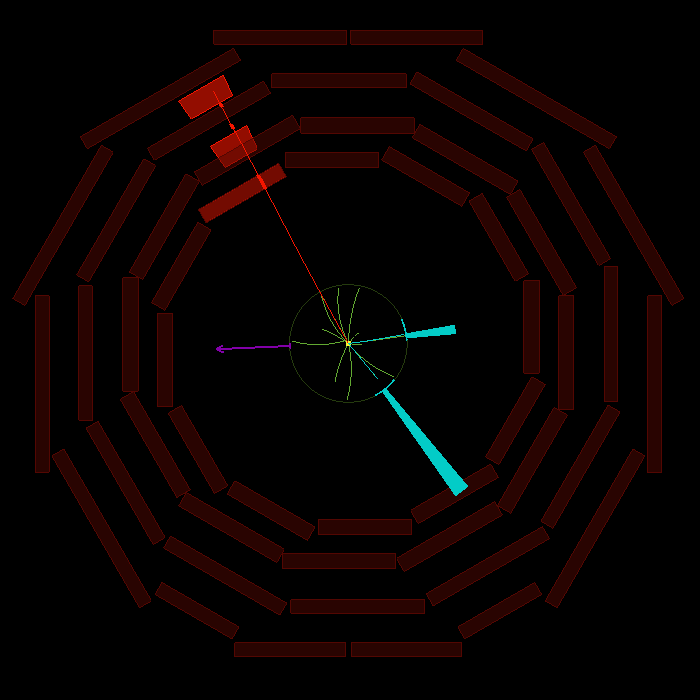
\includegraphics[width=0.8\linewidth]{fig/Fireworks/B_RhoPhi.png}}
  \vfil
  \subfigure[Projection on the $\rho-z$ plane\label{fig:B_RhoZ}]{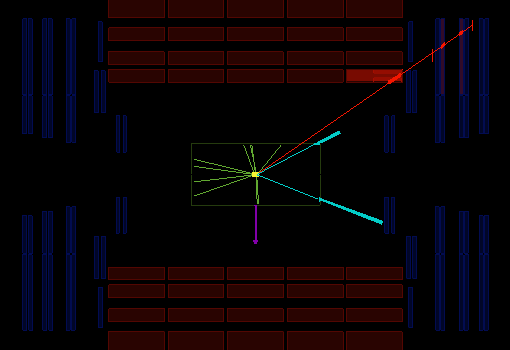
\includegraphics[width=0.40\linewidth]{fig/Fireworks/B_RhoZ.png}}
  \subfigure[3D view\label{fig:B_Rho3D}]{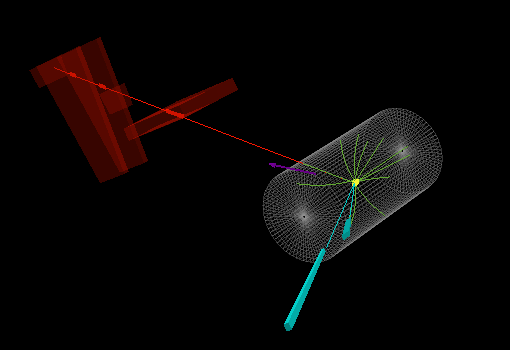
\includegraphics[width=0.40\linewidth]{fig/Fireworks/B_3D.png}}
  \caption{Example of the signature left on the detector by a signal-like event
    for the $ee\mu\nu$ channel. This event was taken on October 21st 2018. Run: $32500$,
    Lumiblock: $188$, Event: $346288517$. The reconstructed primary vertex is shown in yellow.
    Depositions on the electromagnetic calorimeter
    and tracks left by the electronic pair are shown in cyan, the negligible curvature
    shown by their tracks is a reflection of their high transverse momentum, the cyan
    area is proportional to the amount of energy deposited in the calorimeter. Tracks left by the muon
    in the tracker detector and muon chambers are shown in red, in this particular event it
    is possible to see the muon will be classified as a global-High Pt muon as its hits
    are found in the tracker system and beyond the first station of the muon subsystem.
    The amount of missing
    transverse energy is proportional to the length of the purple arrow. Low momentum
    tracks for particle-flow candidates in the inner tracker are shown in green for
    reference, these PF candidates are filtered by the preselection. }
  \label{fig:Fireworks_eemuv}
\end{figure}

\begin{figure}
  \centering
  \subfigure[Projection on the $\rho-\phi$ plane. \label{fig:C_RhoPhi}]{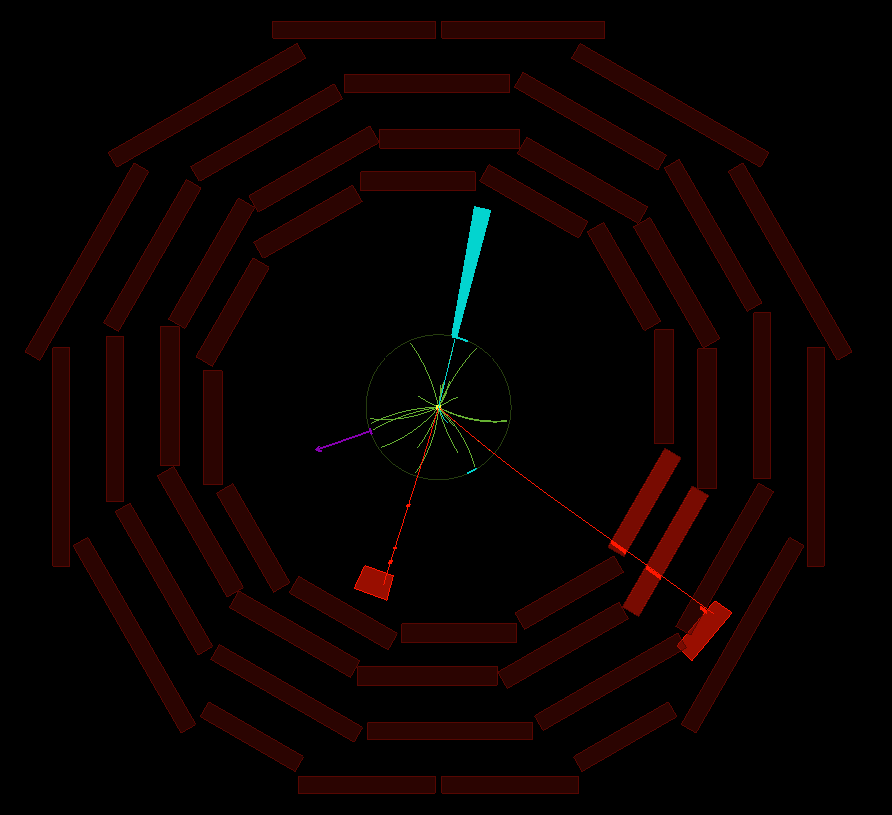
\includegraphics[width=0.8\linewidth]{fig/Fireworks/Cv2_RhoPhi.png}}
  \vfil
  \subfigure[Projection on the $\rho-z$ plane\label{fig:C_RhoZ}]{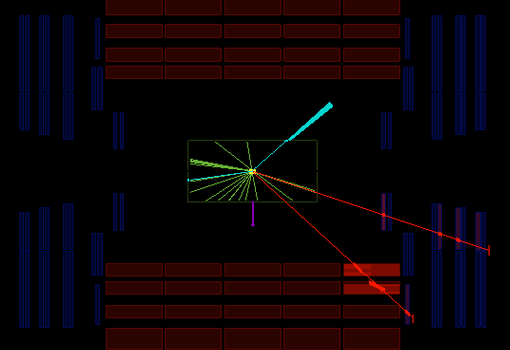
\includegraphics[width=0.40\linewidth]{fig/Fireworks/Cv2_RhoZ.png}}
  \subfigure[3D view\label{fig:C_Rho3D}]{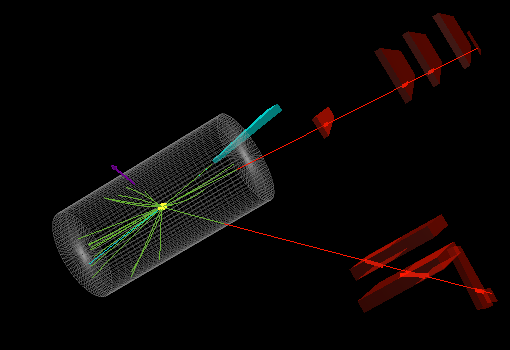
\includegraphics[width=0.40\linewidth]{fig/Fireworks/Cv2_3D.png}}
  \caption{Example of the signature left on the detector by a signal-like event
    for the $\mu\mu e \nu$ channel. This event was taken on October 1st 2018.
    Run: $323790$, Lumiblock: $376$, Event: $646065569$. The reconstructed primary vertex is shown in yellow.
    The deposition on the electromagnetic calorimeter and tracks left by the electron are shown in cyan,
    the negligible curvature shown by their tracks is a reflection of their high transverse momentum.
    Tracks left by the muon pair in the tracker detector and muon chambers are shown in red.
    Both muons would be classified as global-High Pt Muon as their hits
    go beyond the first station of the muon subsystem. The amount of missing
    transverse energy is proportional to the length of the purple arrow. Low momentum
    tracks for particle-flow candidates in the inner tracker are shown in green for
    reference, these PF candidates are filtered by the preselection. }
  \label{fig:Fireworks_mumuev}
\end{figure}

\begin{figure}
  \centering
  \subfigure[Projection on the $\rho-\phi$ plane. \label{fig:D_RhoPhi}]{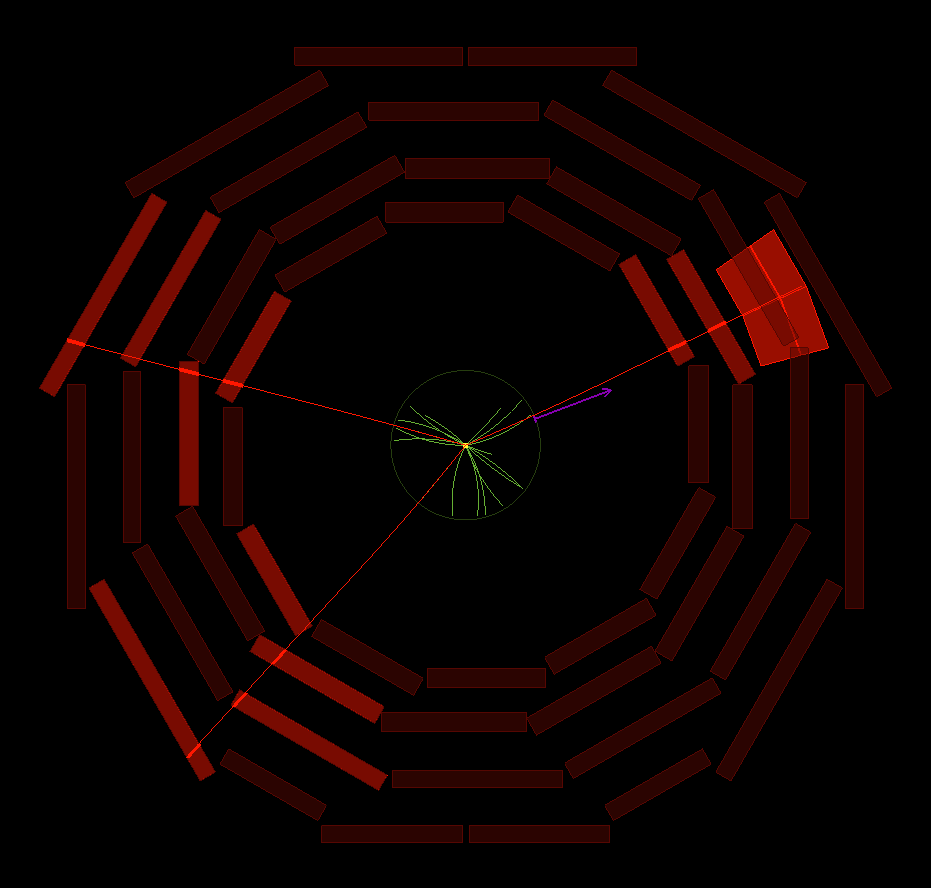
\includegraphics[width=0.8\linewidth]{fig/Fireworks/D_RhoPhi.png}}
  \vfil
  \subfigure[Projection on the $\rho-z$ plane\label{fig:D_RhoZ}]{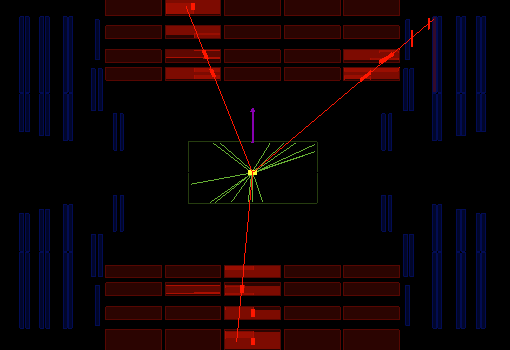
\includegraphics[width=0.40\linewidth]{fig/Fireworks/D_RhoZ.png}}
  \subfigure[3D view\label{fig:D_Rho3D}]{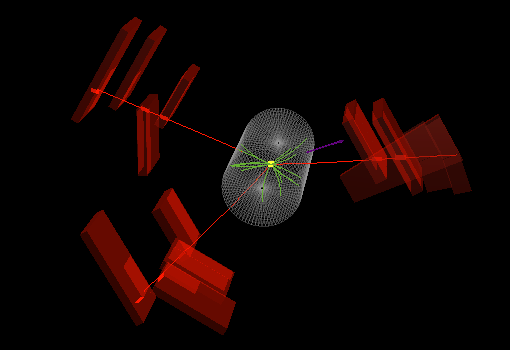
\includegraphics[width=0.40\linewidth]{fig/Fireworks/D_3D.png}}
  \caption{Example of the signature left on the detector by a signal-like event
    for the $\mu\mu\mu\nu$ channel. This event was taken on July 21st 2018.
    Run: $320024$, Lumiblock: $211$, Event: $355149645$. The reconstructed primary vertex is shown in yellow.
    Tracks left by the muon pair in the tracker detector and muon chambers are shown in red,
    the negligible curvature shown by their tracks is a reflection of their high transverse momentum.
    it is possible to see the muon will be classified as a global-High Pt muon as their hits
    are found in the tracker system and beyond the first station of the muon subsystem.
    The amount of missing
    transverse energy is proportional to the length of the purple arrow. Low momentum
    tracks for particle-flow candidates in the inner tracker are shown in green for
    reference, these PF candidates are filtered by the preselection. }
  \label{fig:Fireworks_mumumuv}
\end{figure}




\section{Corrections on MC}

\subsection{Luminosity Scale factors}

The number of generated MC events listed on tables \ref{tab:BkgList2016}, \ref{tab:BkgList2017},
and \ref{tab:BkgList2018} are arbitrary. In order to compare it with data, the
former has to be rescaled to account for the amount of data collected each year
during the data taking period. The luminosity scale factor is computed as follows:

\begin{equation}
  L_{sf}=\frac{L_{\rm data}}{L_{\rm MC}} = \frac{L_{\rm data}\times\sigma_{\rm MC}}{n_{\rm MC}},
\label{eq:lumiSF}
\end{equation}

Where $L_{\rm data}$ is the luminosity per year, see table \ref{tab:LuminosityPerYear},
$n_{MC}$ the number of generated MC events as provided by the sum of weighted events
from the generator (\verb|genWeight| branch on \verb|NanoAOD|), and $\sigma_{\rm MC}$
is the cross section of the MC samples as provided by \verb|XSecAnalyzer|.

\subsection{Pileup Reweighting}

\begin{figure}[tph]
  \centering
        \subfigure[Standard model WZ production normalized pileup distributions for Run 2 years]{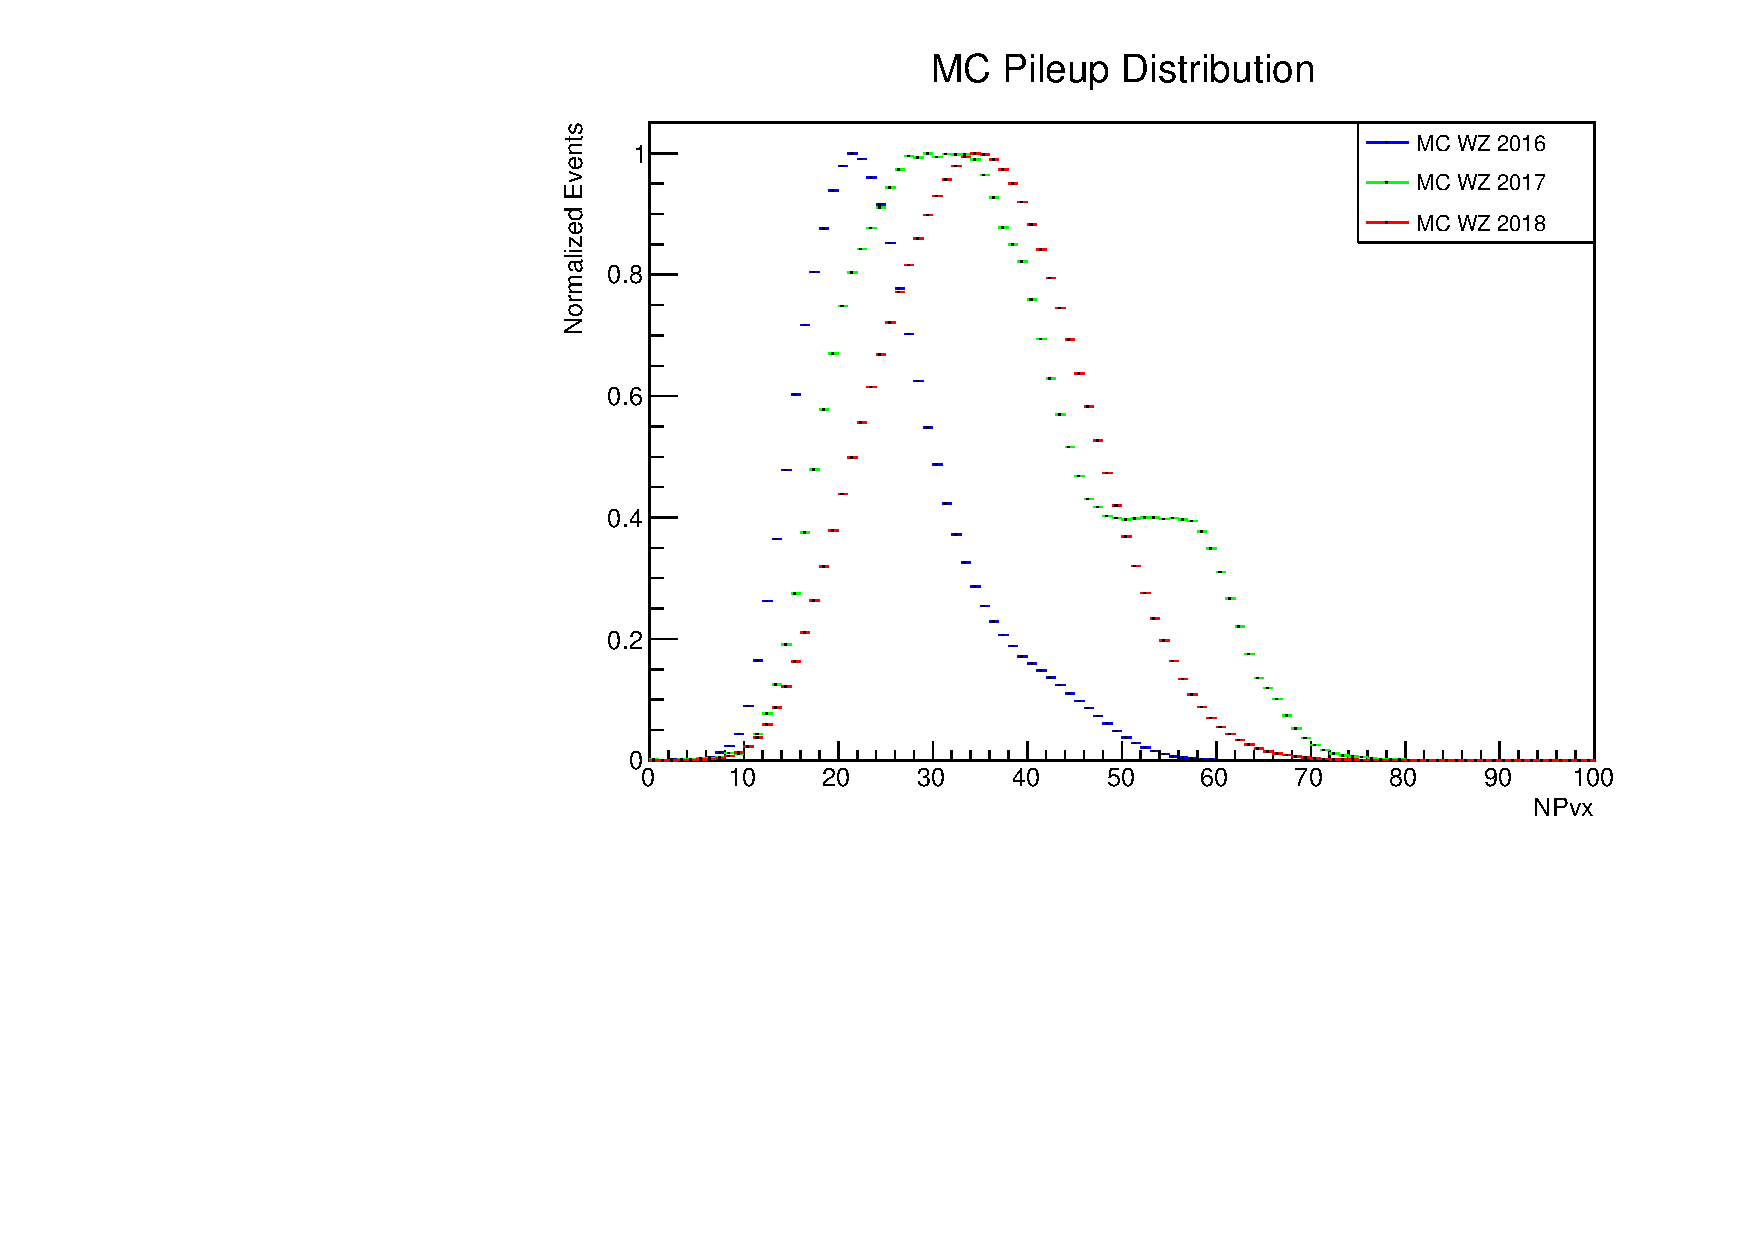
\includegraphics[width=.5\textwidth]{fig/ScaleFactors/MC_Pileup_Linear.pdf}}
        \subfigure[Pileup profile from Run 2 Data, Linear Scale]{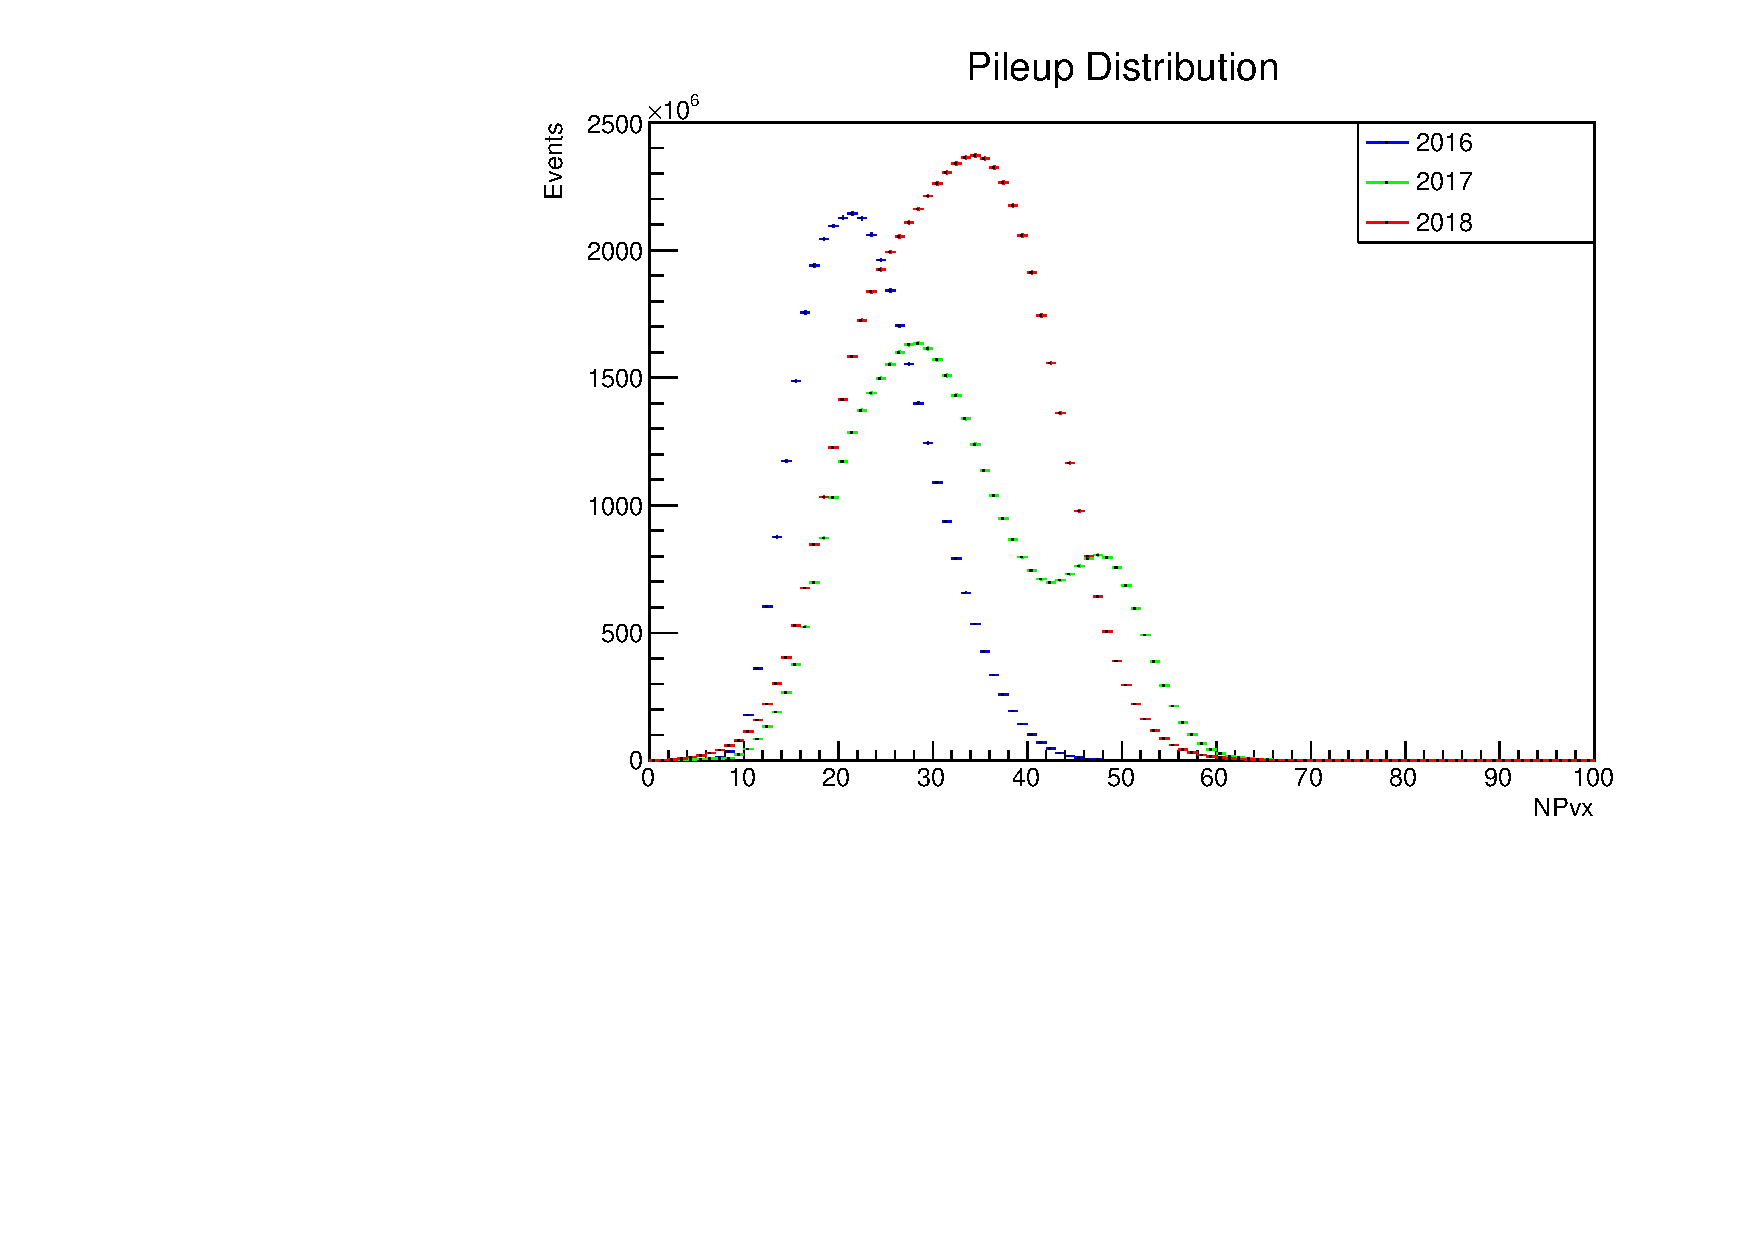
\includegraphics[width=.5\textwidth]{fig/ScaleFactors/GoldenPileup_Linear.pdf}}
        \vfil
        \subfigure[Pileup profile from Run 2 Data, Logarithmic Scale]{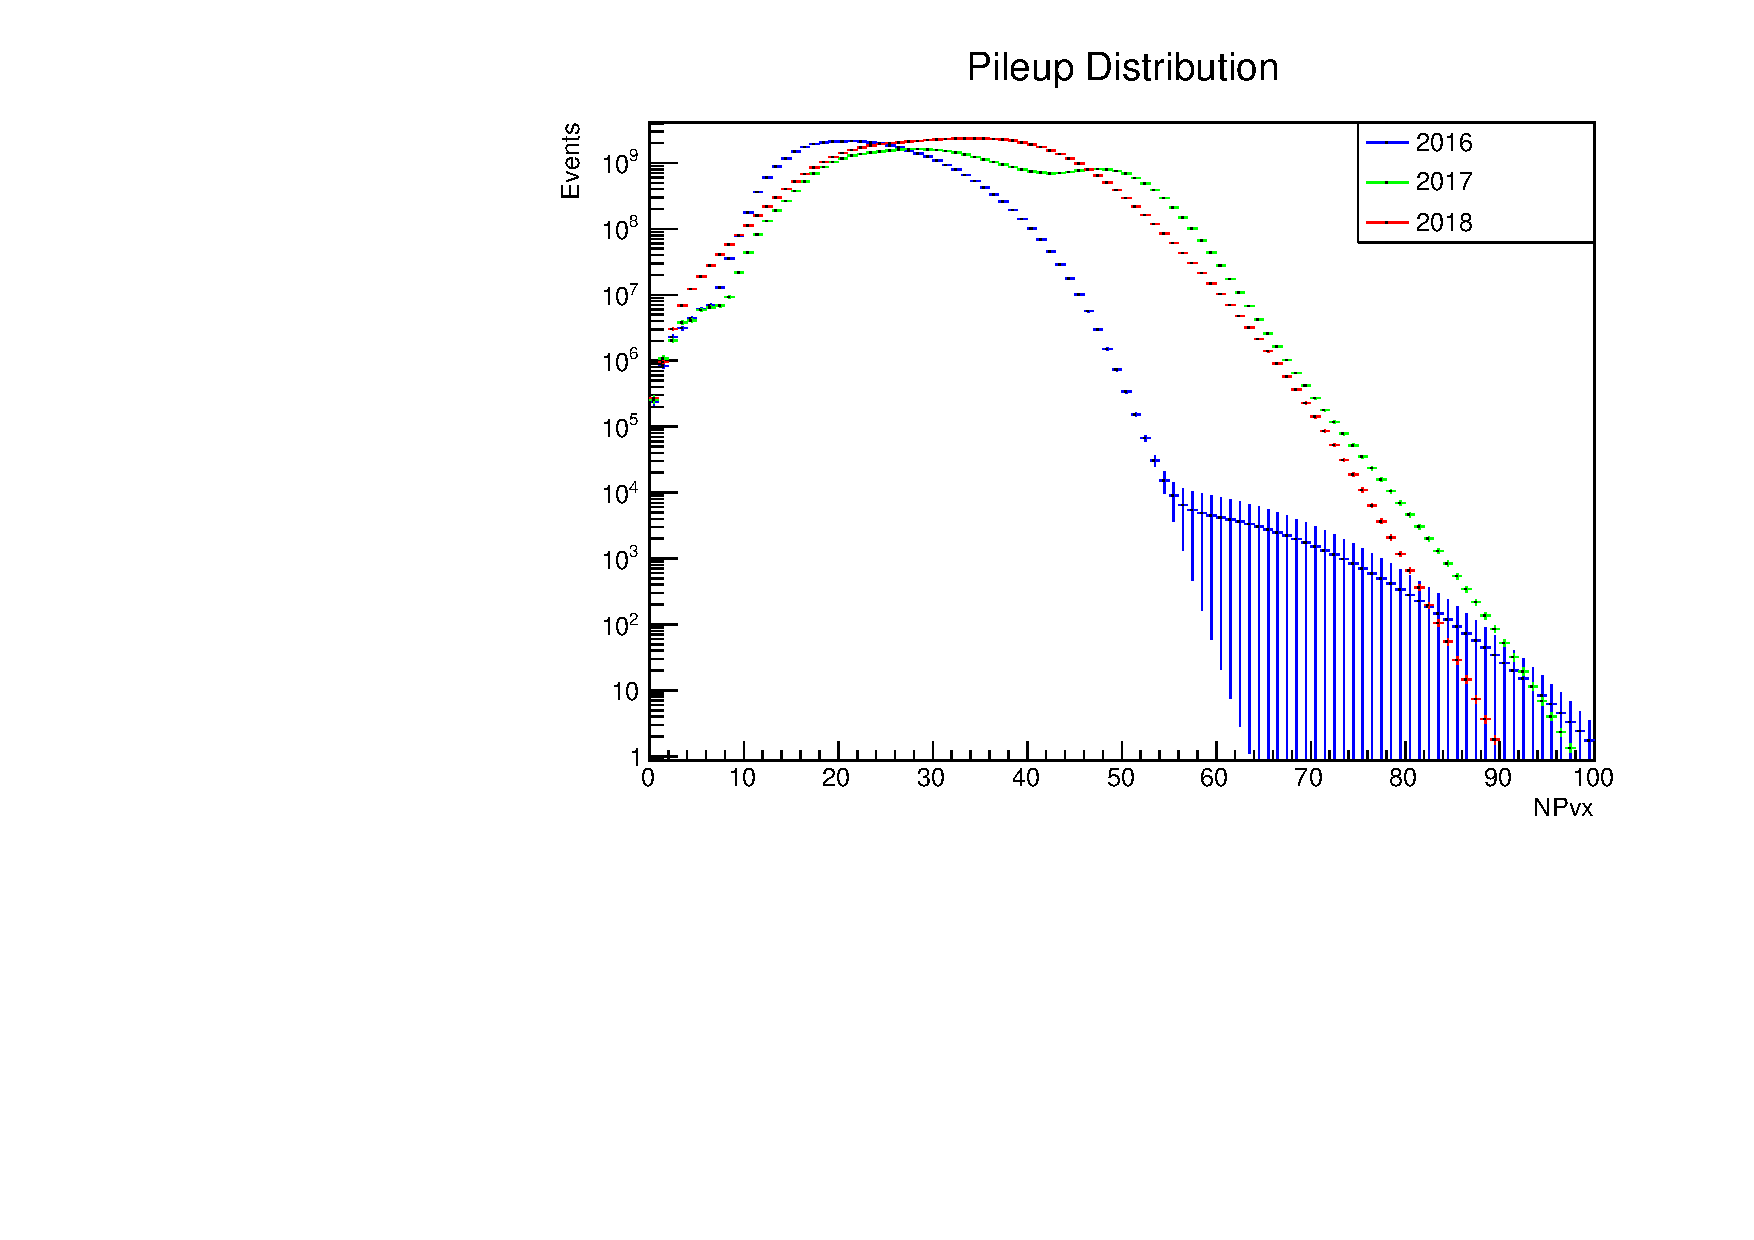
\includegraphics[width=.5\textwidth]{fig/ScaleFactors/GoldenPileup_LogScale.pdf}}
        \subfigure[Pileup weight profiles for several background samples]{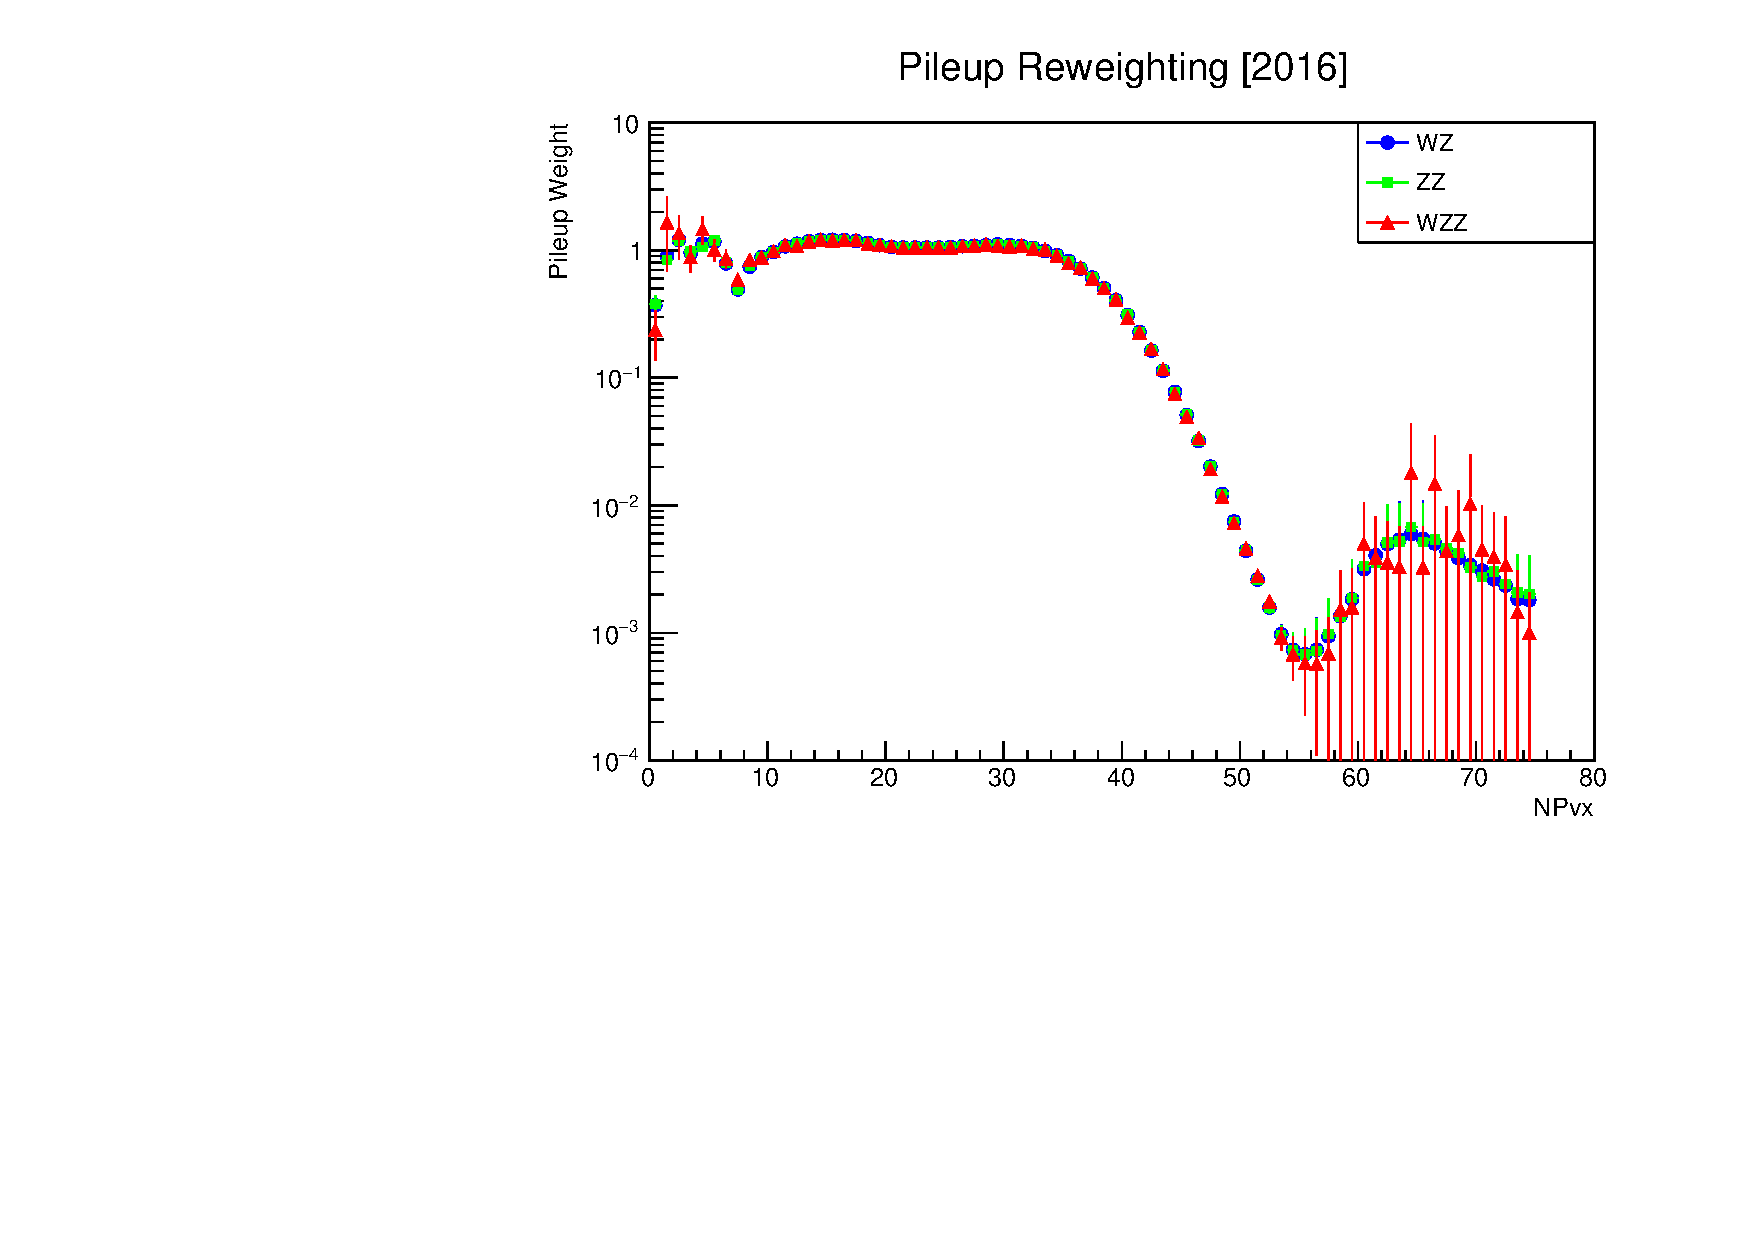
\includegraphics[width=.5\textwidth]{fig/ScaleFactors/PileupWeight_LogScale.pdf}}
  \caption{Pileup profile distributions for MC and Data}
  \label{fig:RunII_PileupProfiles}
\end{figure}

The number of reconstructed primary vertices in each collision during a period
of time generates a distribution commonly referred as pileup. Montecarlo simulations
are produced with an estimated pileup profile and a correction is needed
in order to match the distributions obtained in the collected data.
MC Samples are reweighted with $69.2~mb$ as MinBias cross section \cite{pureweight}.
Figure \ref{fig:RunII_PileupProfiles} shows the differences between the
pileup distributions for run 2 data and montecarlo
simulations for the predominant background process (standard model
WZ production). These differences are then
corrected by computing a pileup weight bin by bin that matches the normalized
distribution from montecarlo with the normalized distribution from data.
The normalization of each distribution is eachieved by scaling it by a factor
equivalent to the the inverse of its integral. Each MC event is then reweighted
with the appropiate factor based on the number of reconstructed primary vertices. 

\subsection{Lepton scale factors}

\begin{figure}[tph]
  \centering
  \subfigure[Electron Loose ID. Applied to the $eee$ and $ee\mu$ channels
    based on the pseudorapidity $\eta$ and transverse momentum $P_{t}$ of each
    of the electrons used to define a $Z$ candidate in the event.
    The applied weight is the product of the scale factors of each individual electron.
  ]{\includegraphics[width=.45\textwidth]{fig/ScaleFactors/2016Electron_LooseID.pdf}}
  \hspace{5mm}
  \subfigure[Electron Tight ID. Applied to the $eee$ and $\mu\mu e$ channels
    based on the pseudorapidity $\eta$ and transverse momentum $P_{t}$ of the
    electron used to define the $W$ candidate.
  ]{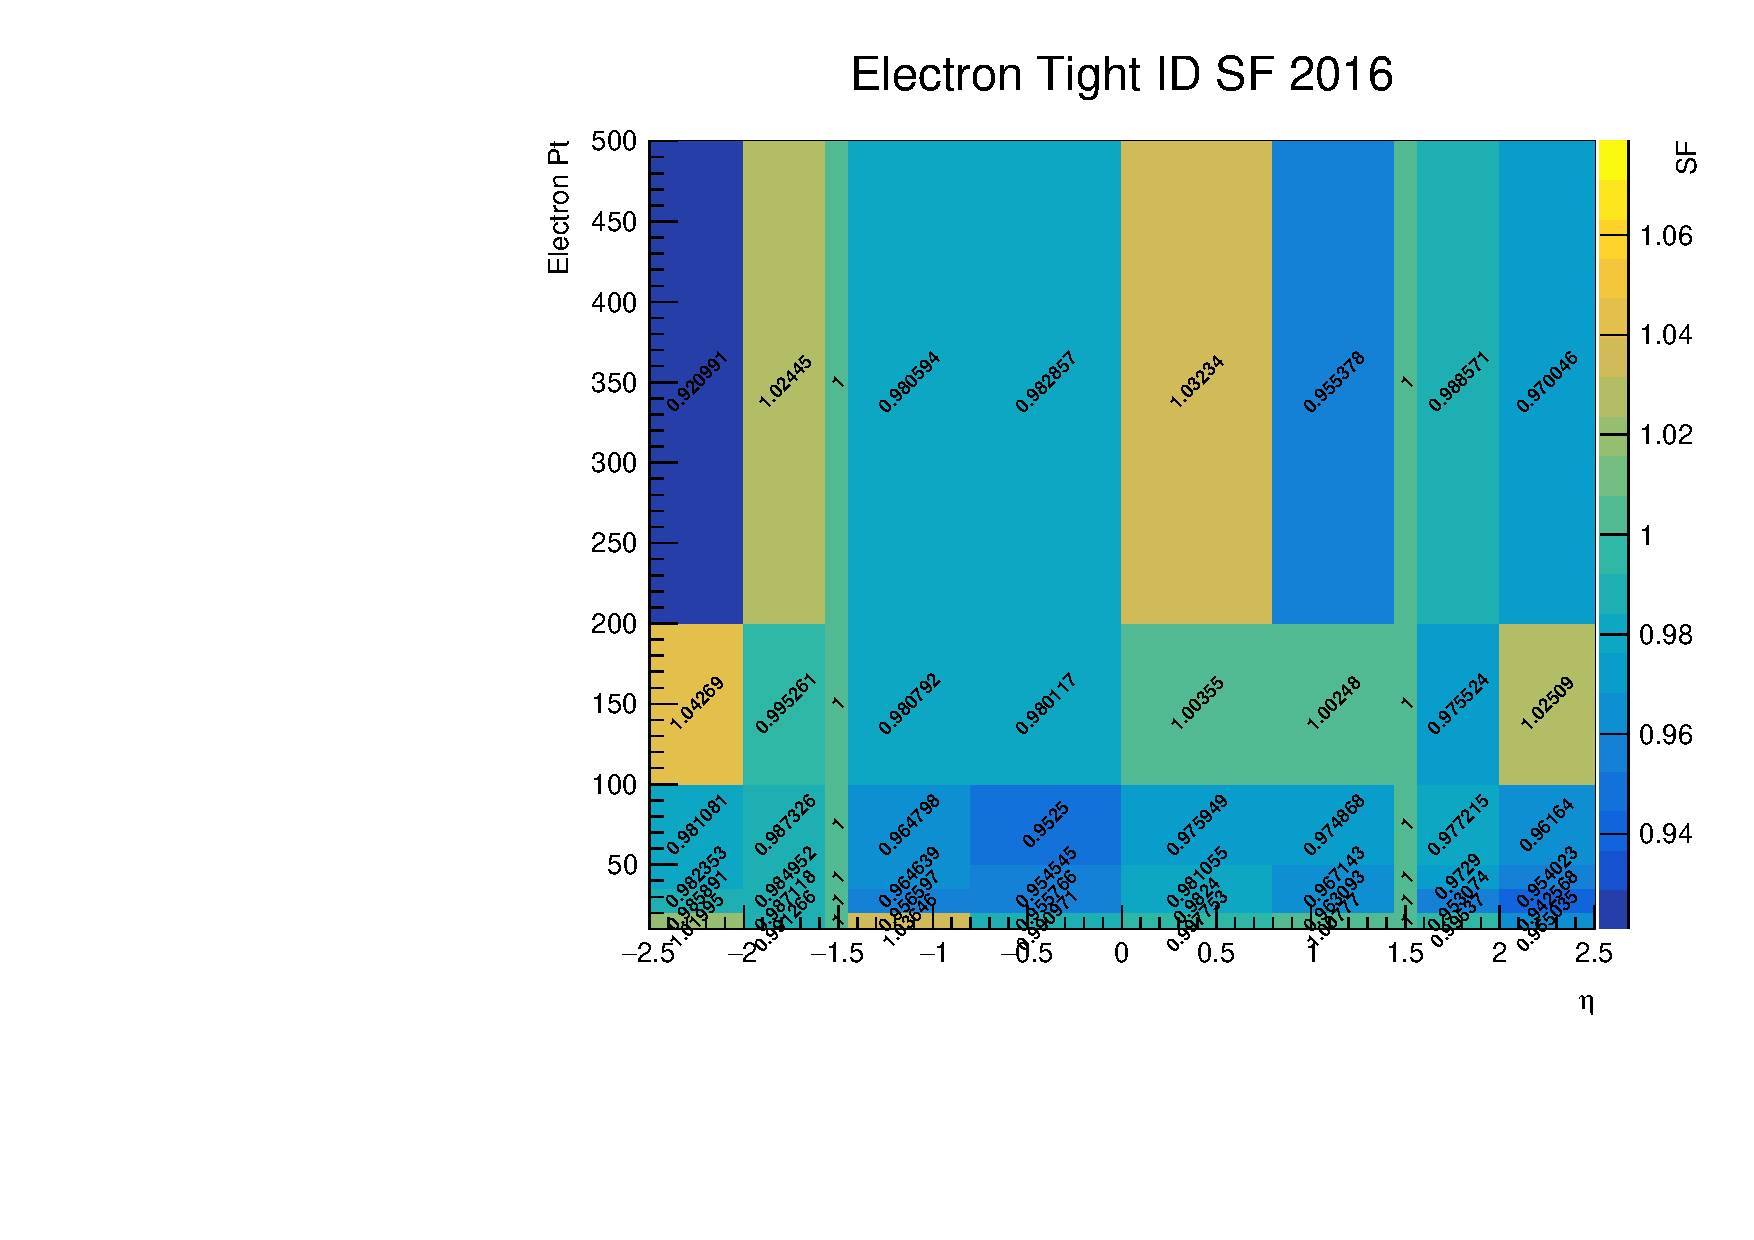
\includegraphics[width=.45\textwidth]{fig/ScaleFactors/2016Electron_TightID.pdf}}
  \vfil
  \subfigure[Muon GlobalHighPtId. Applied to the $\mu\mu e$, $ee\mu$,
    and $\mu\mu\mu$ channels based on the pseudorapidity $\eta$ and transverse
    momentum $P_{t}$ of each of the muons used to define a $WZ$ candidate in the event
    identified as GlobalHighPt.
    The applied weight is the product of the scale factors of each individual muon.
  ]{\includegraphics[width=.45\textwidth]{fig/ScaleFactors/2016Muon_GlobalHighPtID.pdf}}
  \hspace{5mm}
  \subfigure[Muon TrkHighPtId. Applied to the $\mu\mu e$ and $ee\mu$,
     and $\mu\mu\mu$ channels based on the pseudorapidity $\eta$ and transverse
     momentum $P_{t}$ of each of the muons used to define a $WZ$ candidate in the event
     identified as TrackerHighPt.
     The applied weight is the product of the scale factors of each individual muon.
  ]{\includegraphics[width=.45\textwidth]{fig/ScaleFactors/2016Muon_TrkHighPtID.pdf}}
  \caption{Lepton ID Scale Factors 2016}
  \label{fig:leptonidsf_2016}
\end{figure}

\begin{figure}[tph]
  \centering
  \subfigure[Electron Loose ID. Applied to the $eee$ and $ee\mu$ channels
    based on the pseudorapidity $\eta$ and transverse momentum $P_{t}$ of each
    of the electrons used to define a $Z$ candidate in the event.
    The applied weight is the product of the scale factors of each individual electron.
  ]{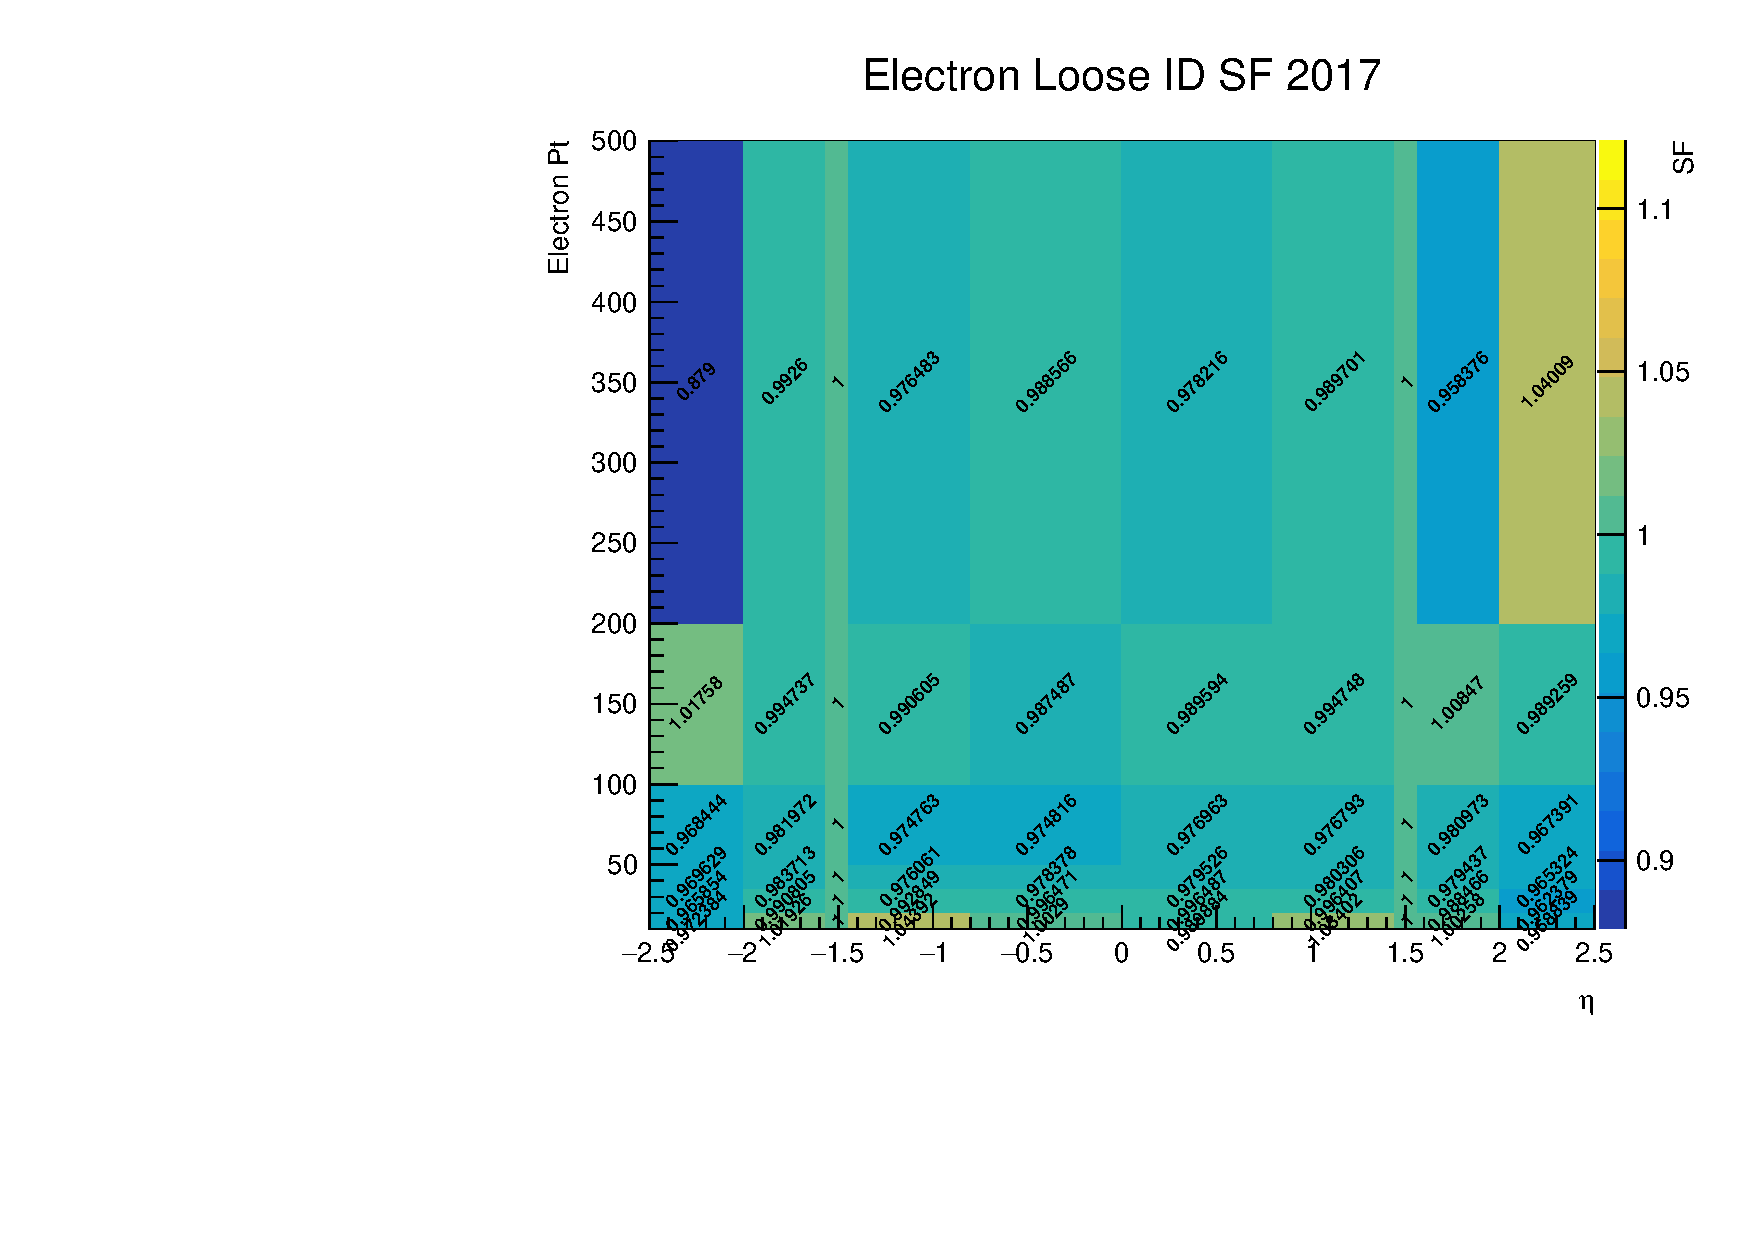
\includegraphics[width=.45\textwidth]{fig/ScaleFactors/2017Electron_LooseID.pdf}}
  \hspace{5mm}
  \subfigure[Electron Tight ID. Applied to the $eee$ and $\mu\mu e$ channels
    based on the pseudorapidity $\eta$ and transverse momentum $P_{t}$ of the
    electron used to define the $W$ candidate.]{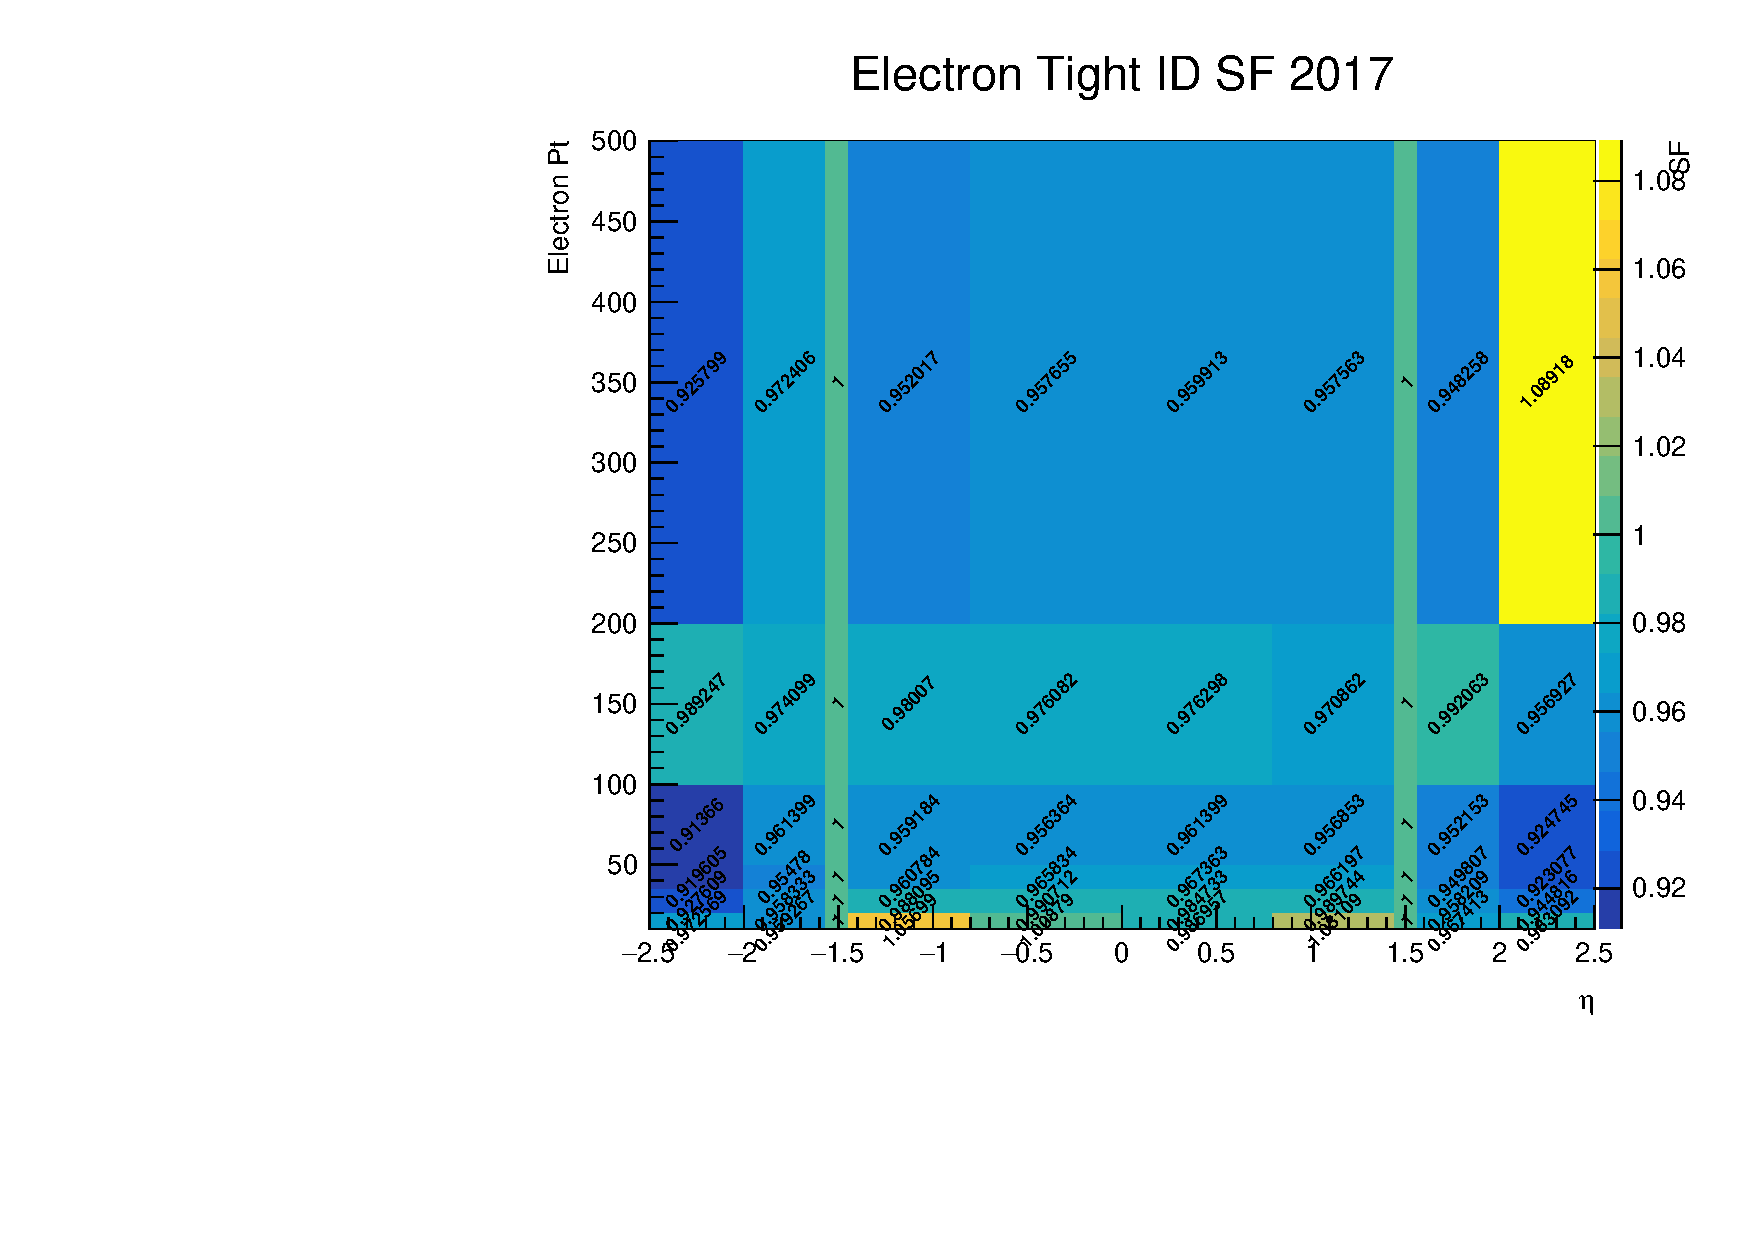
\includegraphics[width=.45\textwidth]{fig/ScaleFactors/2017Electron_TightID.pdf}}
  \vfil
  \subfigure[Muon GlobalHighPtId. Applied to the $\mu\mu e$, $ee\mu$,
    and $\mu\mu\mu$ channels based on the pseudorapidity $\eta$ and transverse
    momentum $P_{t}$ of each of the muons used to define a $WZ$ candidate in the event
    identified as GlobalHighPt.
    The applied weight is the product of the scale factors of each individual muon.
  ]{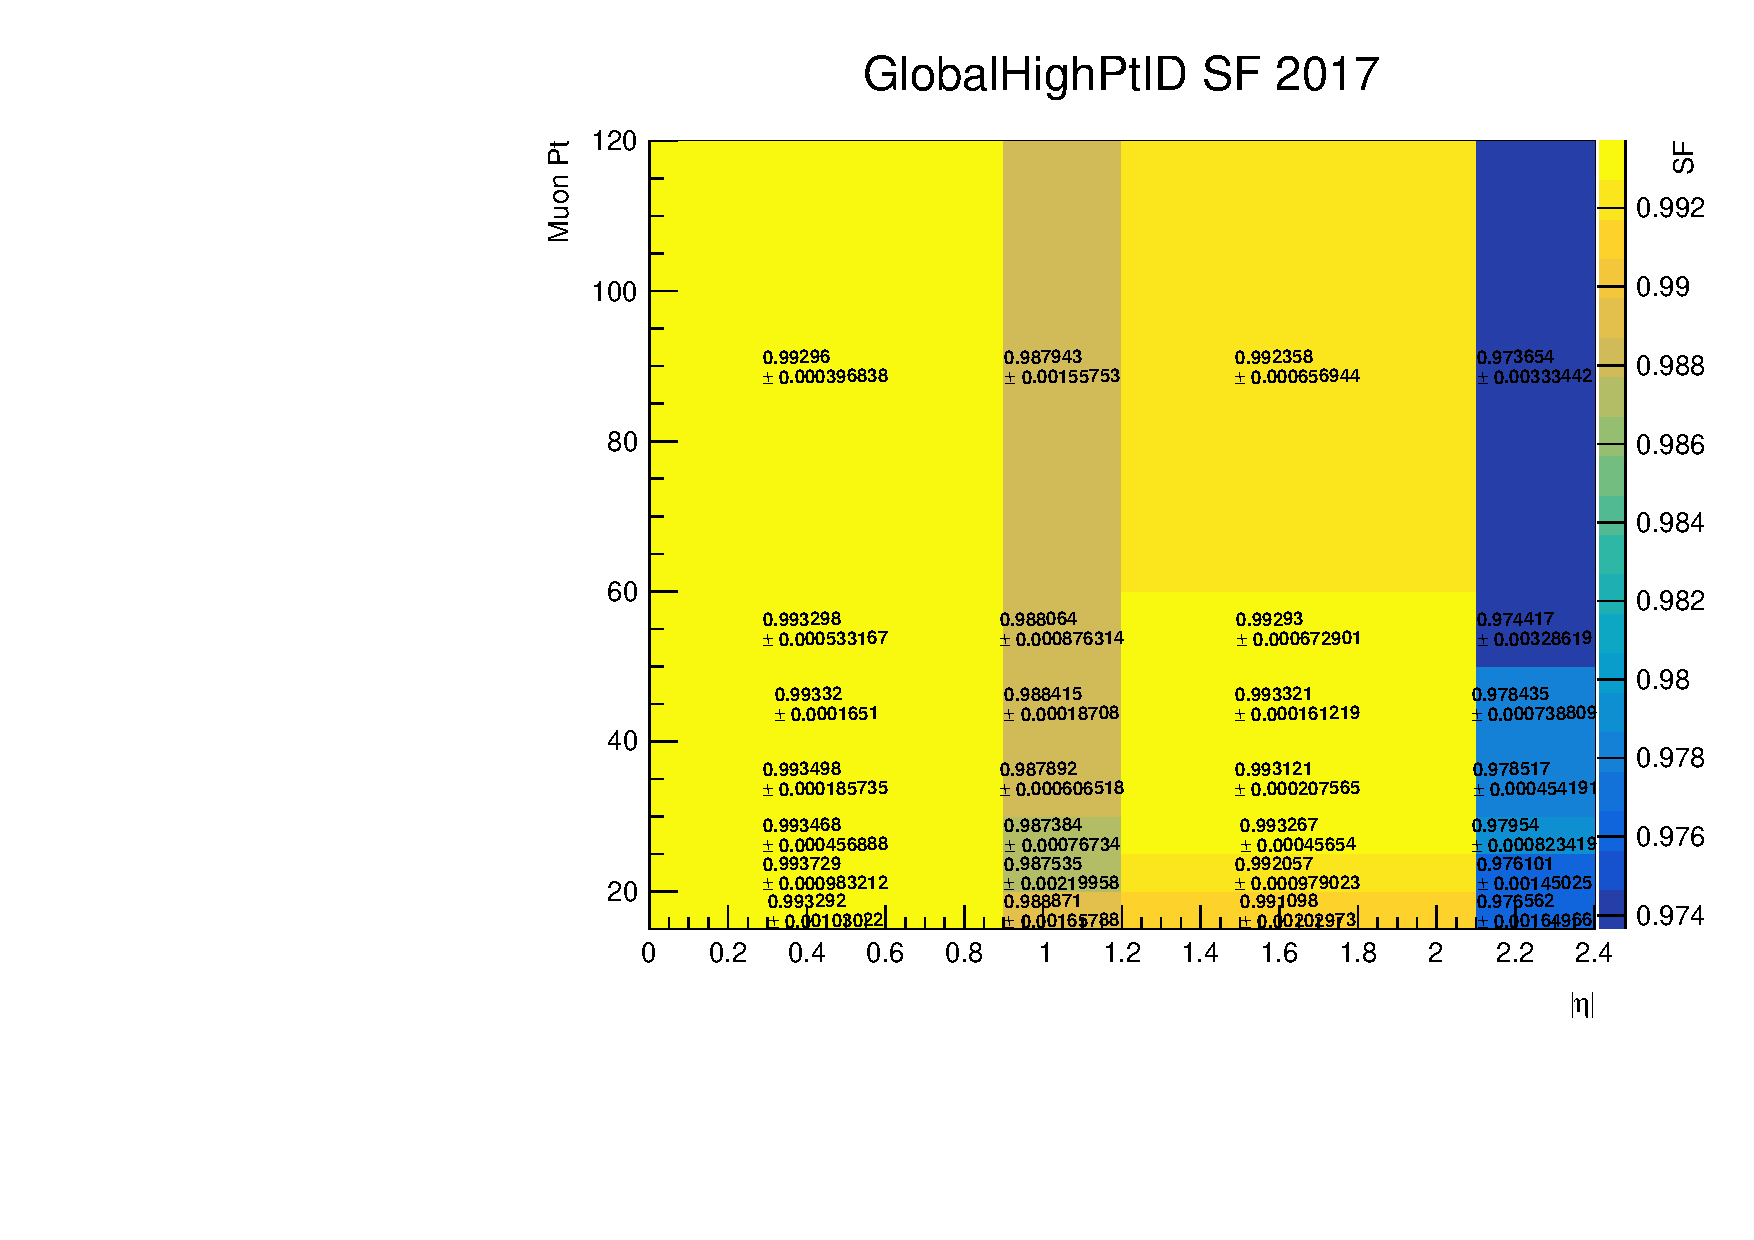
\includegraphics[width=.45\textwidth]{fig/ScaleFactors/2017Muon_GlobalHighPtID.pdf}}
  \hspace{5mm}
  \subfigure[Muon TrkHighPtId. Applied to the $\mu\mu e$ and $ee\mu$,
     and $\mu\mu\mu$ channels based on the pseudorapidity $\eta$ and transverse
     momentum $P_{t}$ of each of the muons used to define a $WZ$ candidate in the event
     identified as TrackerHighPt.
    The applied weight is the product of the scale factors of each individual muon.
  ]{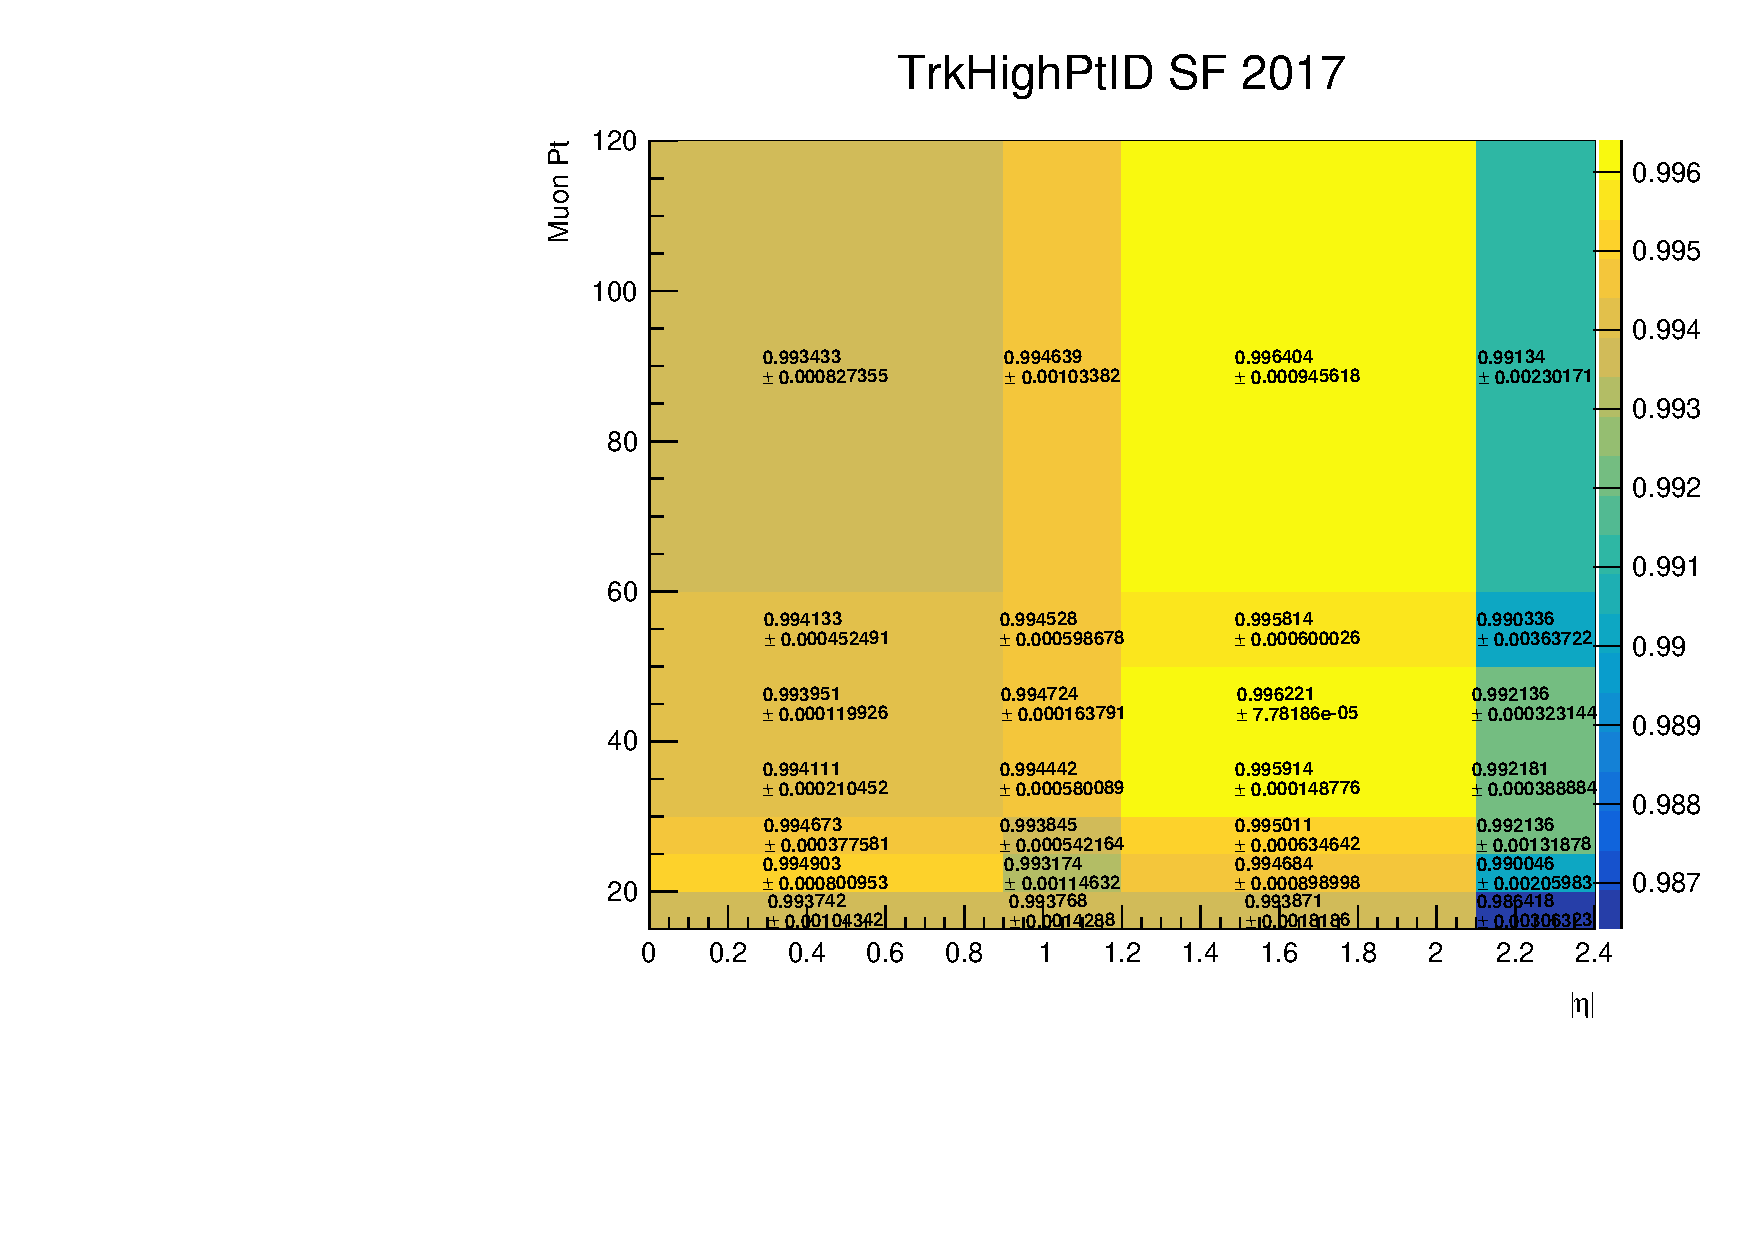
\includegraphics[width=.45\textwidth]{fig/ScaleFactors/2017Muon_TrkHighPtID.pdf}}
  \caption{Lepton ID Scale Factors 2017}
  \label{fig:leptonidsf_2017}
\end{figure}

\begin{figure}[tph]
  \centering
  \subfigure[Electron Loose ID. Applied to the $eee$ and $ee\mu$ channels
    based on the pseudorapidity $\eta$ and transverse momentum $P_{t}$ of each
    of the electrons used to define a $Z$ candidate in the event.
    The applied weight is the product of the scale factors of each individual electron.
  ]{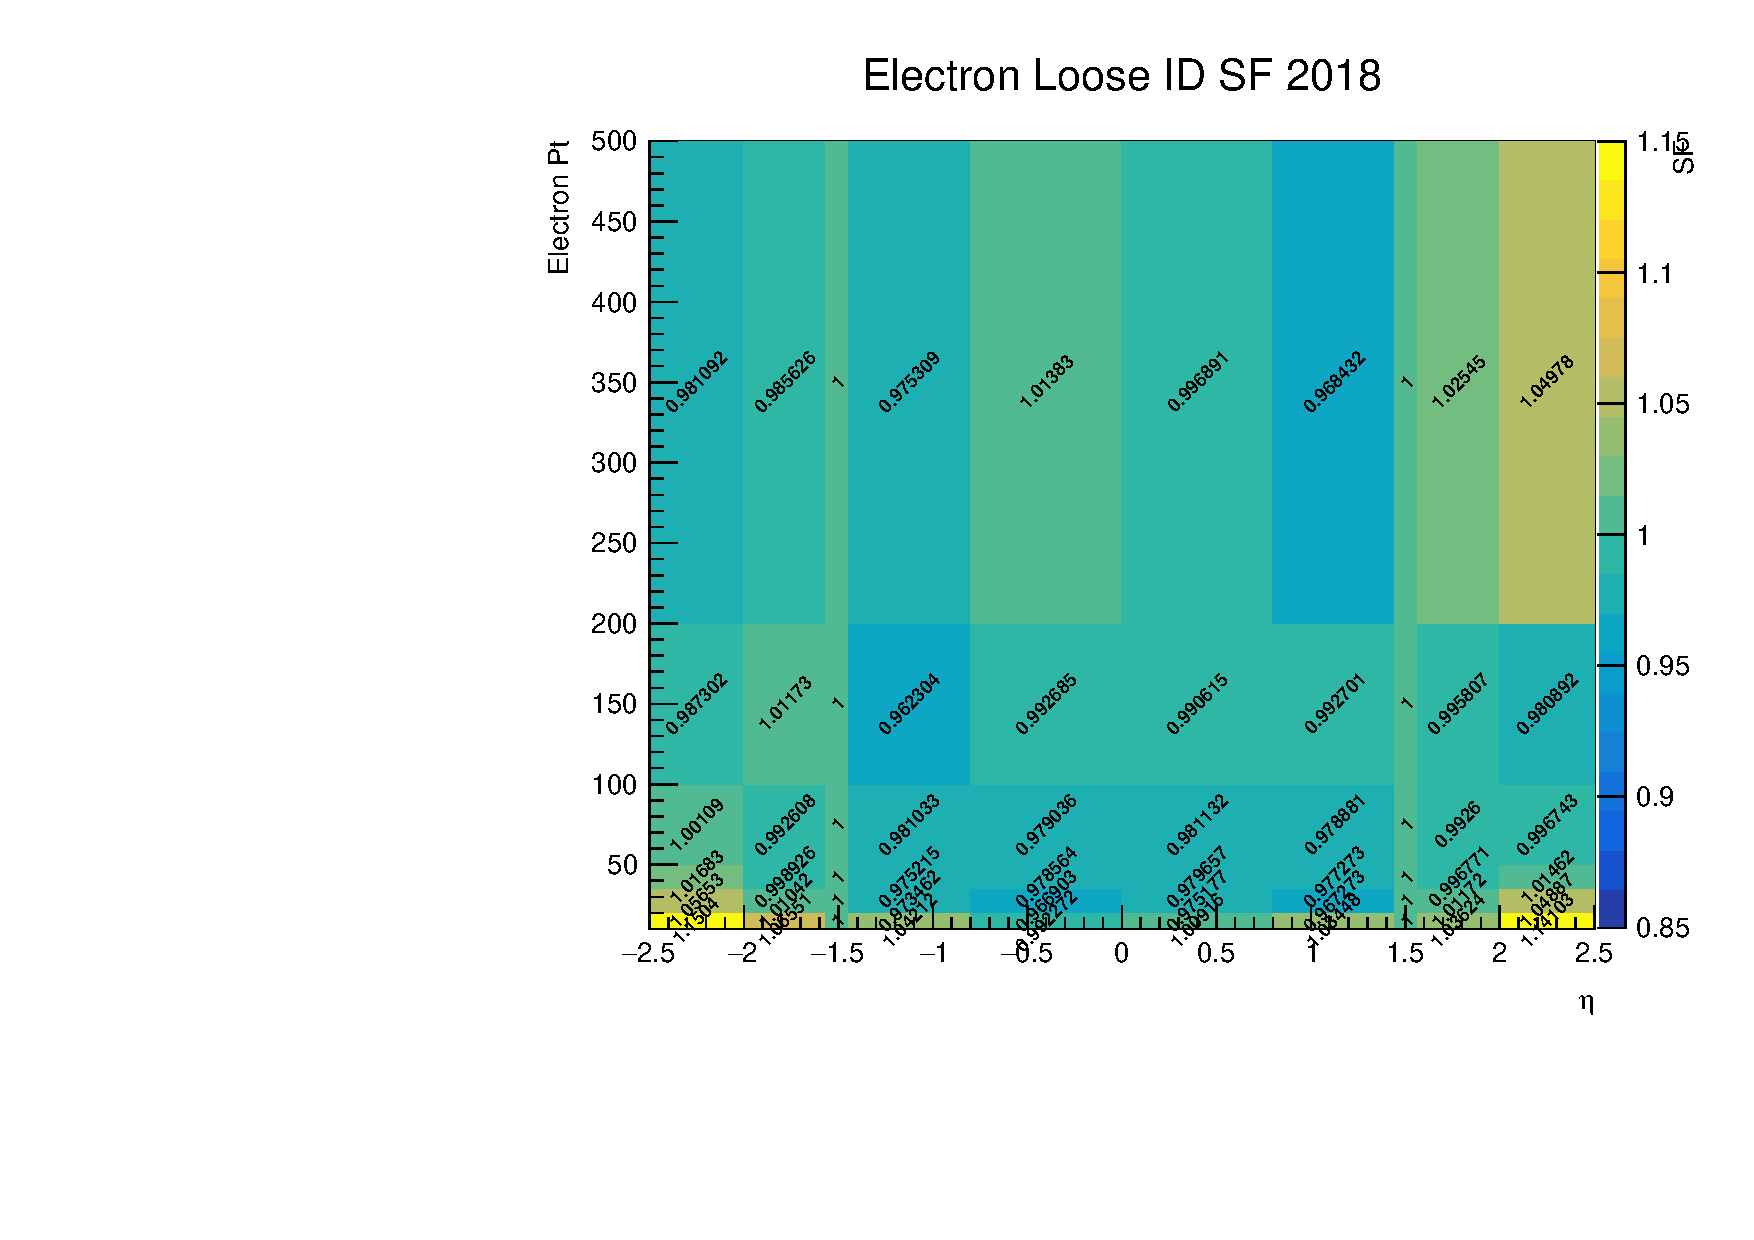
\includegraphics[width=.45\textwidth]{fig/ScaleFactors/2018Electron_LooseID.pdf}}
  \hspace{5mm}
  \subfigure[Electron Tight ID. Applied to the $eee$ and $\mu\mu e$ channels
    based on the pseudorapidity $\eta$ and transverse momentum $P_{t}$ of the
    electron used to define the $W$ candidate.]{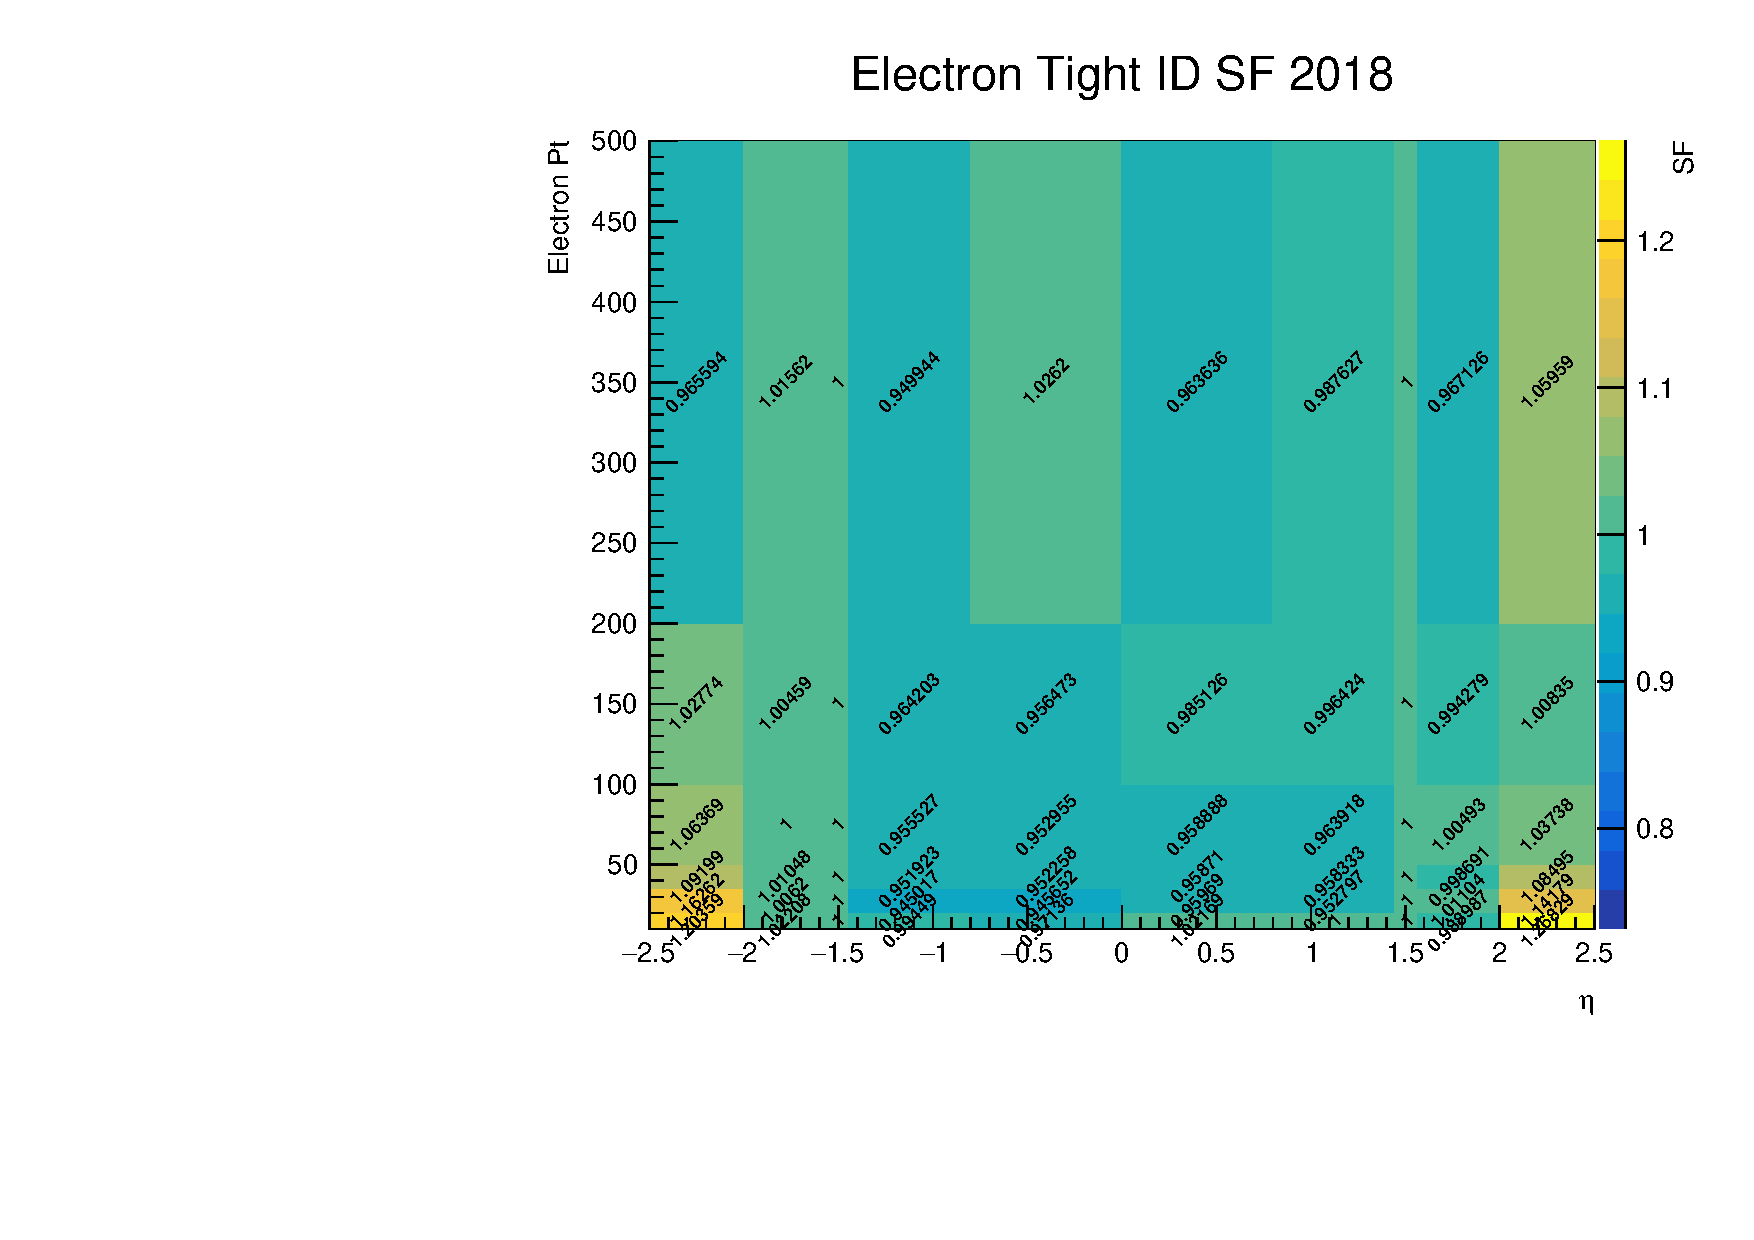
\includegraphics[width=.45\textwidth]{fig/ScaleFactors/2018Electron_TightID.pdf}}
  \vfil
  \subfigure[Muon GlobalHighPtId. Applied to the $\mu\mu e$, $ee\mu$,
    and $\mu\mu\mu$ channels based on the pseudorapidity $\eta$ and transverse
    momentum $P_{t}$ of each of the muons used to define a $WZ$ candidate in the event
    identified as GlobalHighPt.
    The applied weight is the product of the scale factors of each individual muon.
  ]{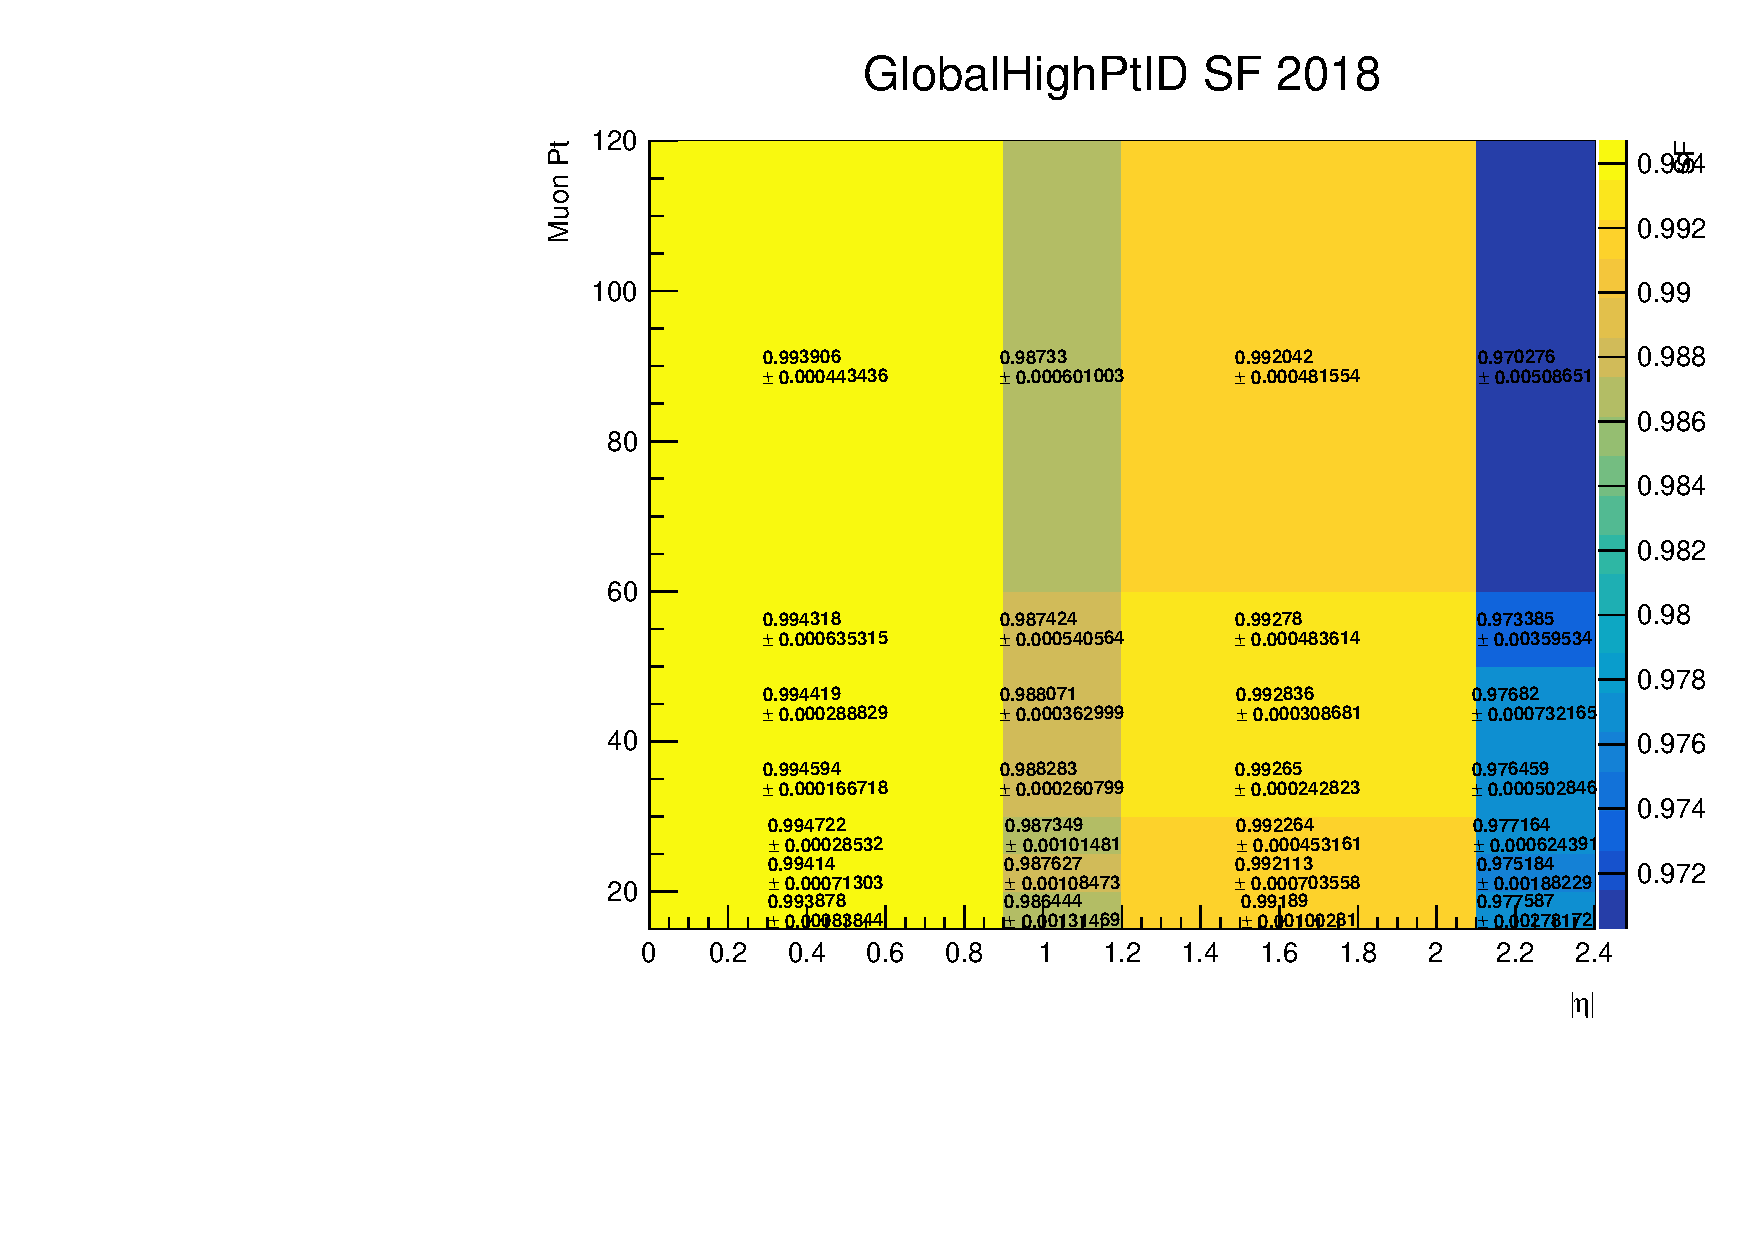
\includegraphics[width=.45\textwidth]{fig/ScaleFactors/2018Muon_GlobalHighPtID.pdf}}
  \hspace{5mm}
  \subfigure[Muon TrkHighPtId. Applied to the $\mu\mu e$ and $ee\mu$,
     and $\mu\mu\mu$ channels based on the pseudorapidity $\eta$ and transverse
     momentum $P_{t}$ of each of the muons used to define a $WZ$ candidate in the event
     identified as TrackerHighPt.
     The applied weight is the product of the scale factors of each individual muon.
  ]{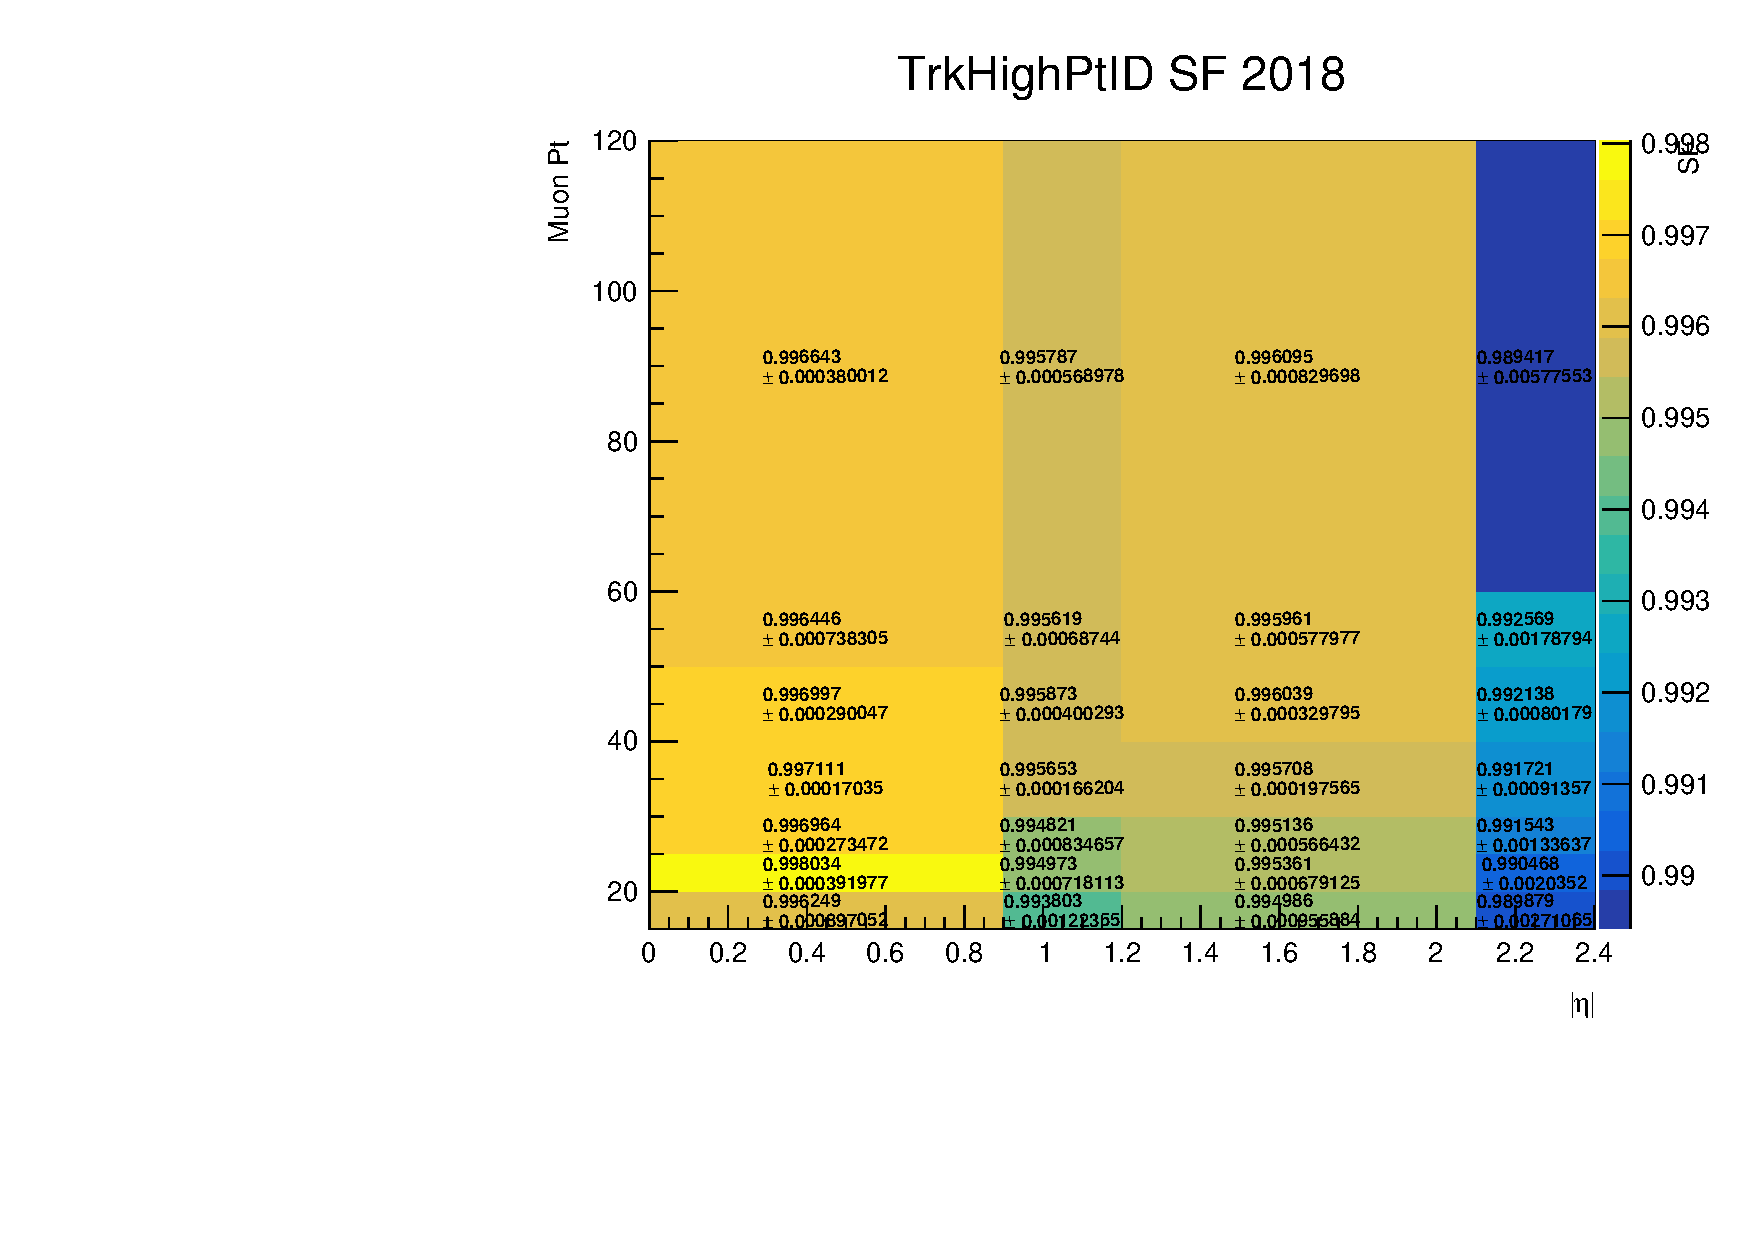
\includegraphics[width=.45\textwidth]{fig/ScaleFactors/2018Muon_TrkHighPtID.pdf}}
  \caption{Lepton ID Scale Factors 2018}
  \label{fig:leptonidsf_2018}
\end{figure}

Trigger and lepton identification efficiencies are different between data
and montecarlo. Scale factors are provided centrally by the Muon and EGamma POG
and show an $\eta-P_{t}$ dependence, see Figures \ref{fig:leptonidsf_2016},
\ref{fig:leptonidsf_2017}, and \ref{fig:leptonidsf_2018}.

The lepton identification scale factor is applied to the event
as a result of the product of each individual scale factor for each lepton in
the channel based on its transverse momentum $P_{t}$ and pseudorapidity $\eta$.
The HLT scale factor is applied based on the $P_{t}$ and $\eta$ of the leading
lepton: events corresponding to channels that include muons and electrons
will contain the product of the muon and electron HLT scale factor while events
from channels that include exclusively muon or electrons will be weighted with
the corresponding HLT scale factor.
Trigger and identification systematics are evaluated by moving up
and down the scale factors by their uncertainties. These uncertainties
are considered flat, independent of the resonance mass, and uncorrelated
in terms of lepton flavour.



\section{Control Region}

\begin{figure}[tph]
  \centering
  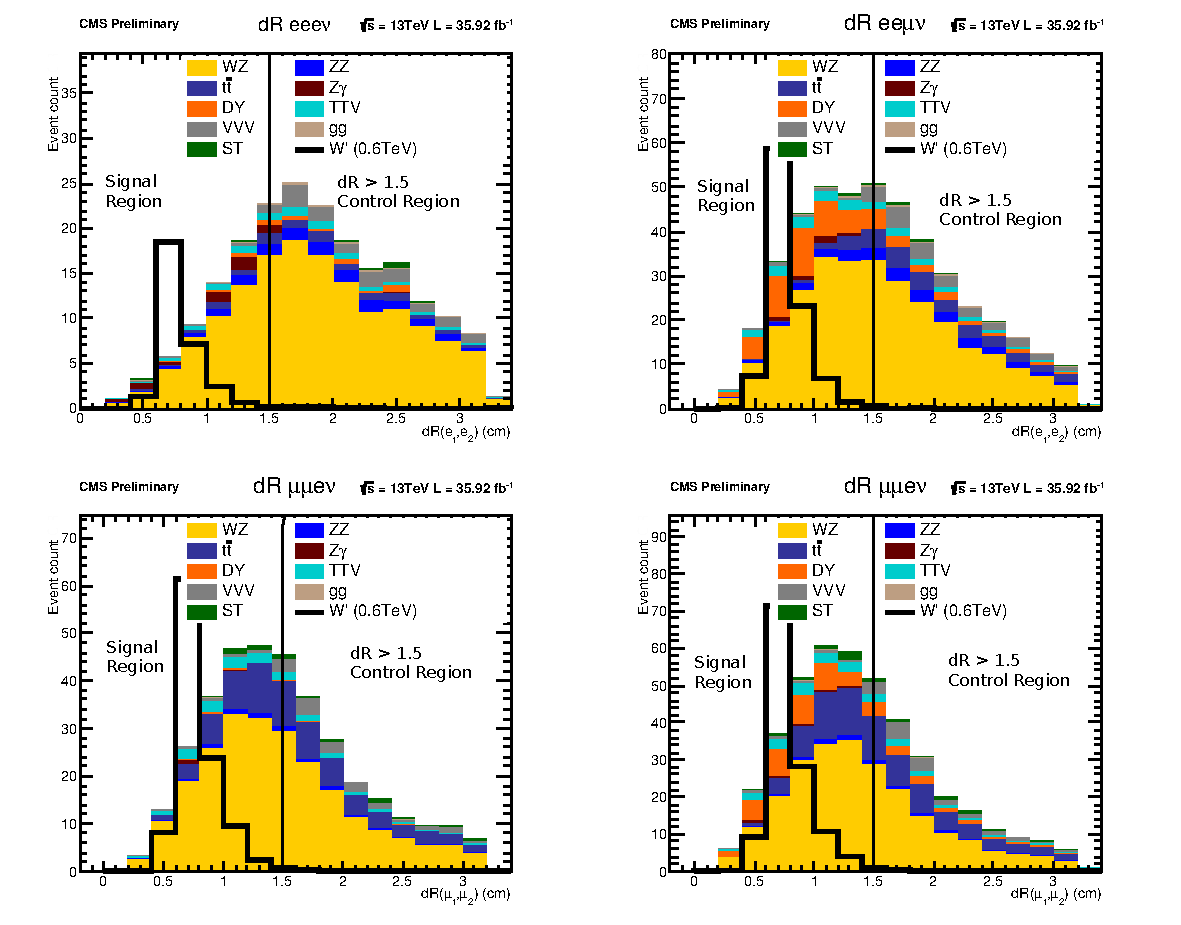
\includegraphics[width=\textwidth]{fig/Run2/KFactorIncluded_HDistl1l2_CR1_A+HDisM600.pdf}
  \caption{Definition of the signal and control regions. All the channels
    show how the region $dr_{l_{1}l_{2}} > 1.5$ is signal-depleted. A $600 GeV$
    mass resonance is used for illustration purposes. The larger the resonance
    mass, the narrower the signal distribution gets and it is shifted towards
    the lower $dR$ region as the leptons product of the $Z$ decay get closer
    forming a boosted topology.
    Top left: $Z(\rightarrow e+e)W(\rightarrow e+\nu)$
    Top right: $Z(\rightarrow e+e)W(\rightarrow \mu+\nu)$
    Bottom left: $Z(\rightarrow \mu+\mu)W(\rightarrow e+\nu)$
    Bottom right: $Z(\rightarrow \mu+\mu)W(\rightarrow \mu+\nu)$}
  \label{fig:ControlRegionDefinition}
\end{figure}

In order to analyse the simulation quality, the data/MC ratio is studied on
a signal-depleted control region. As Figure \ref{fig:ControlRegionDefinition}
shows, the distance in the $\eta-\phi$ plane between the products
of the Z boson decay $Z(\rightarrow l_{1}+l_{2})$ allow a distinct separation between a signal-enriched
region ($dr_{l_{1}l_{2}} <= 1.5$) and a signal depleted region
($dr_{l_{1}l_{2}} > 1.5$). The signal-delepted region is dominated mainly by
the SM WZ production process. Background yields for the control and signal are
shown on Table \ref{tab:BackgroundYieldsCR} and \ref{tab:BackgroundYieldsSR}

\begin{figure}[tph]
  \centering
  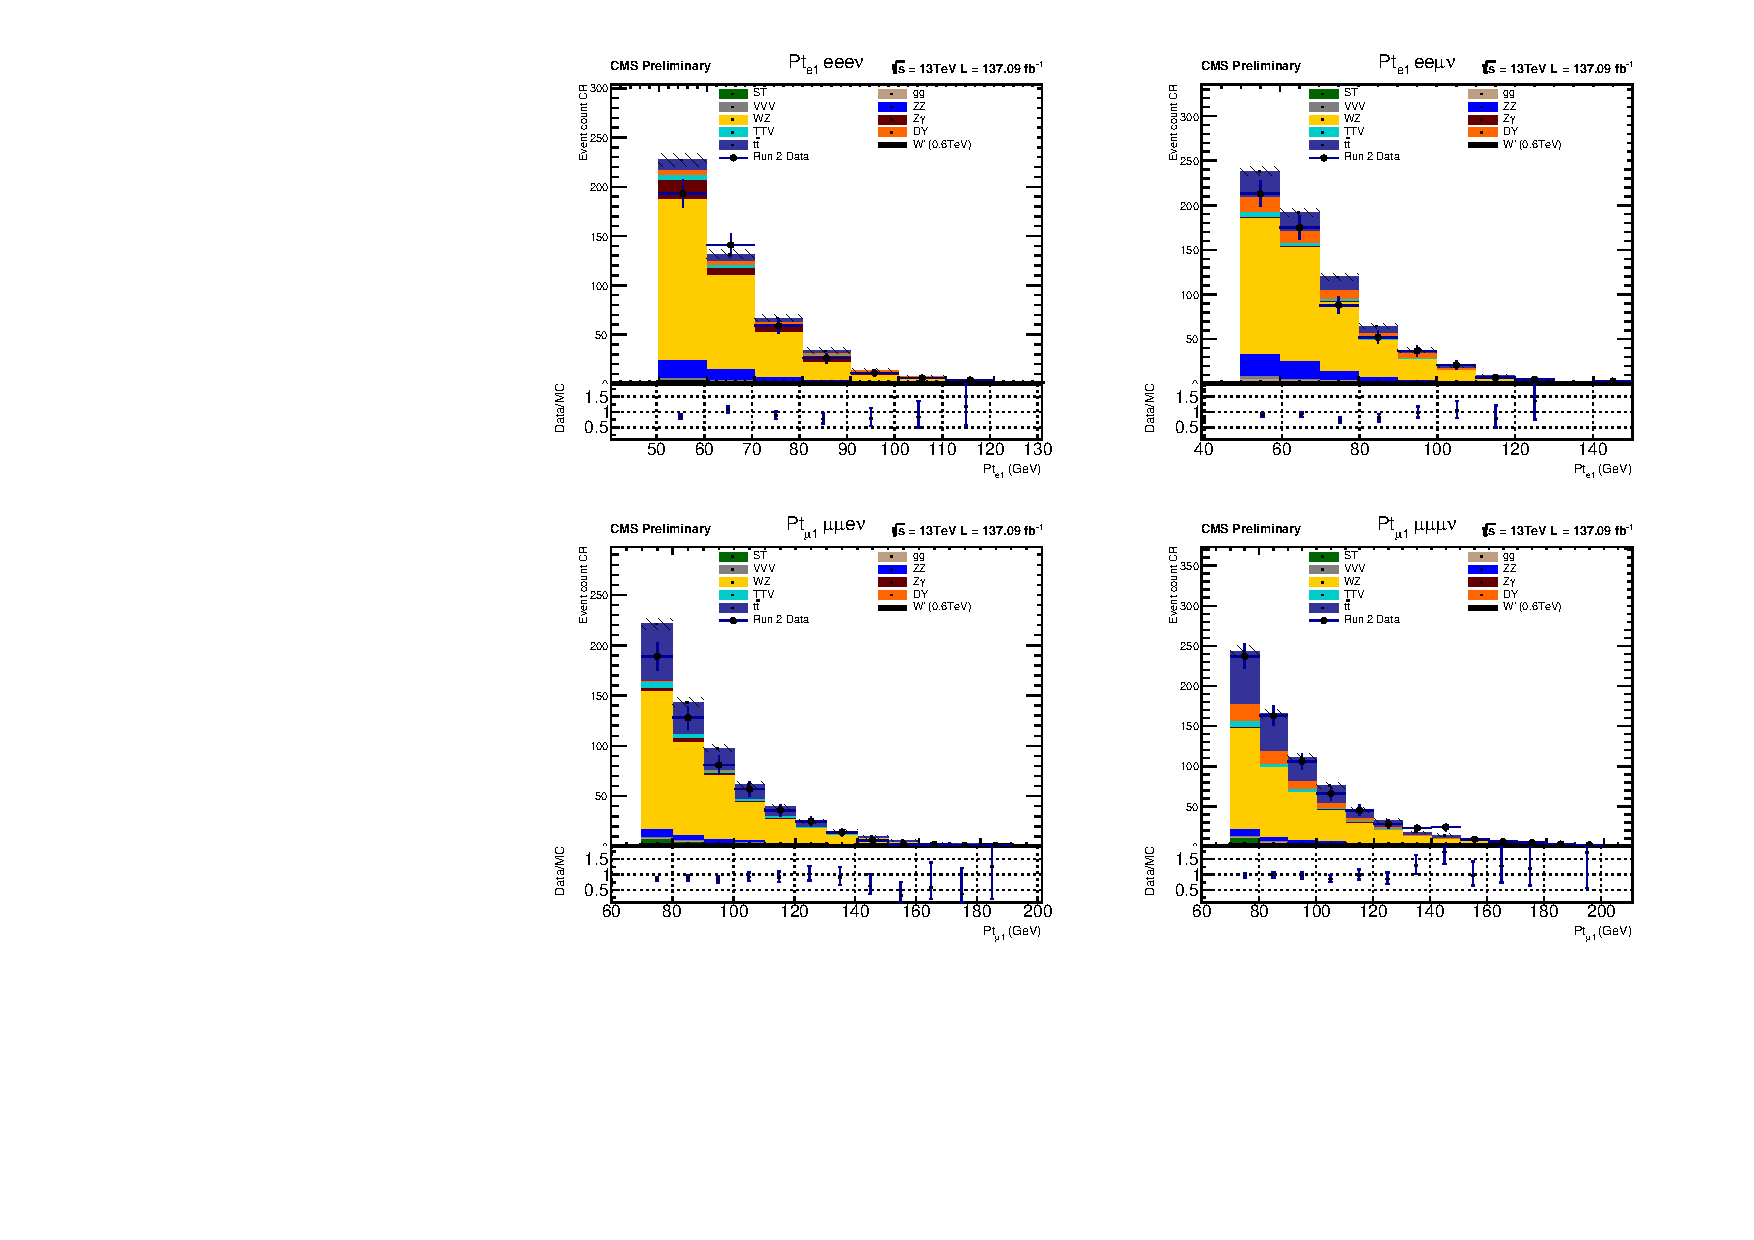
\includegraphics[width=\textwidth]{fig/Run2/KFactorIncluded_HPtl1_CR1_A_Run2_HPtRun2_M600.pdf}
  \caption{Leading lepton transverse momentum distributions for each final
    signature as seen in the $dr_{l_{1}l_{2}} > 1.5$ control region.
    Top left: $Z(\rightarrow e+e)W(\rightarrow e+\nu)$
    Top right: $Z(\rightarrow e+e)W(\rightarrow \mu+\nu)$
    Bottom left: $Z(\rightarrow \mu+\mu)W(\rightarrow e+\nu)$
    Bottom right: $Z(\rightarrow \mu+\mu)W(\rightarrow \mu+\nu)$}
  \label{fig:CR1_Run2_HPtl1}
\end{figure}

\begin{figure}[tph]
  \centering
  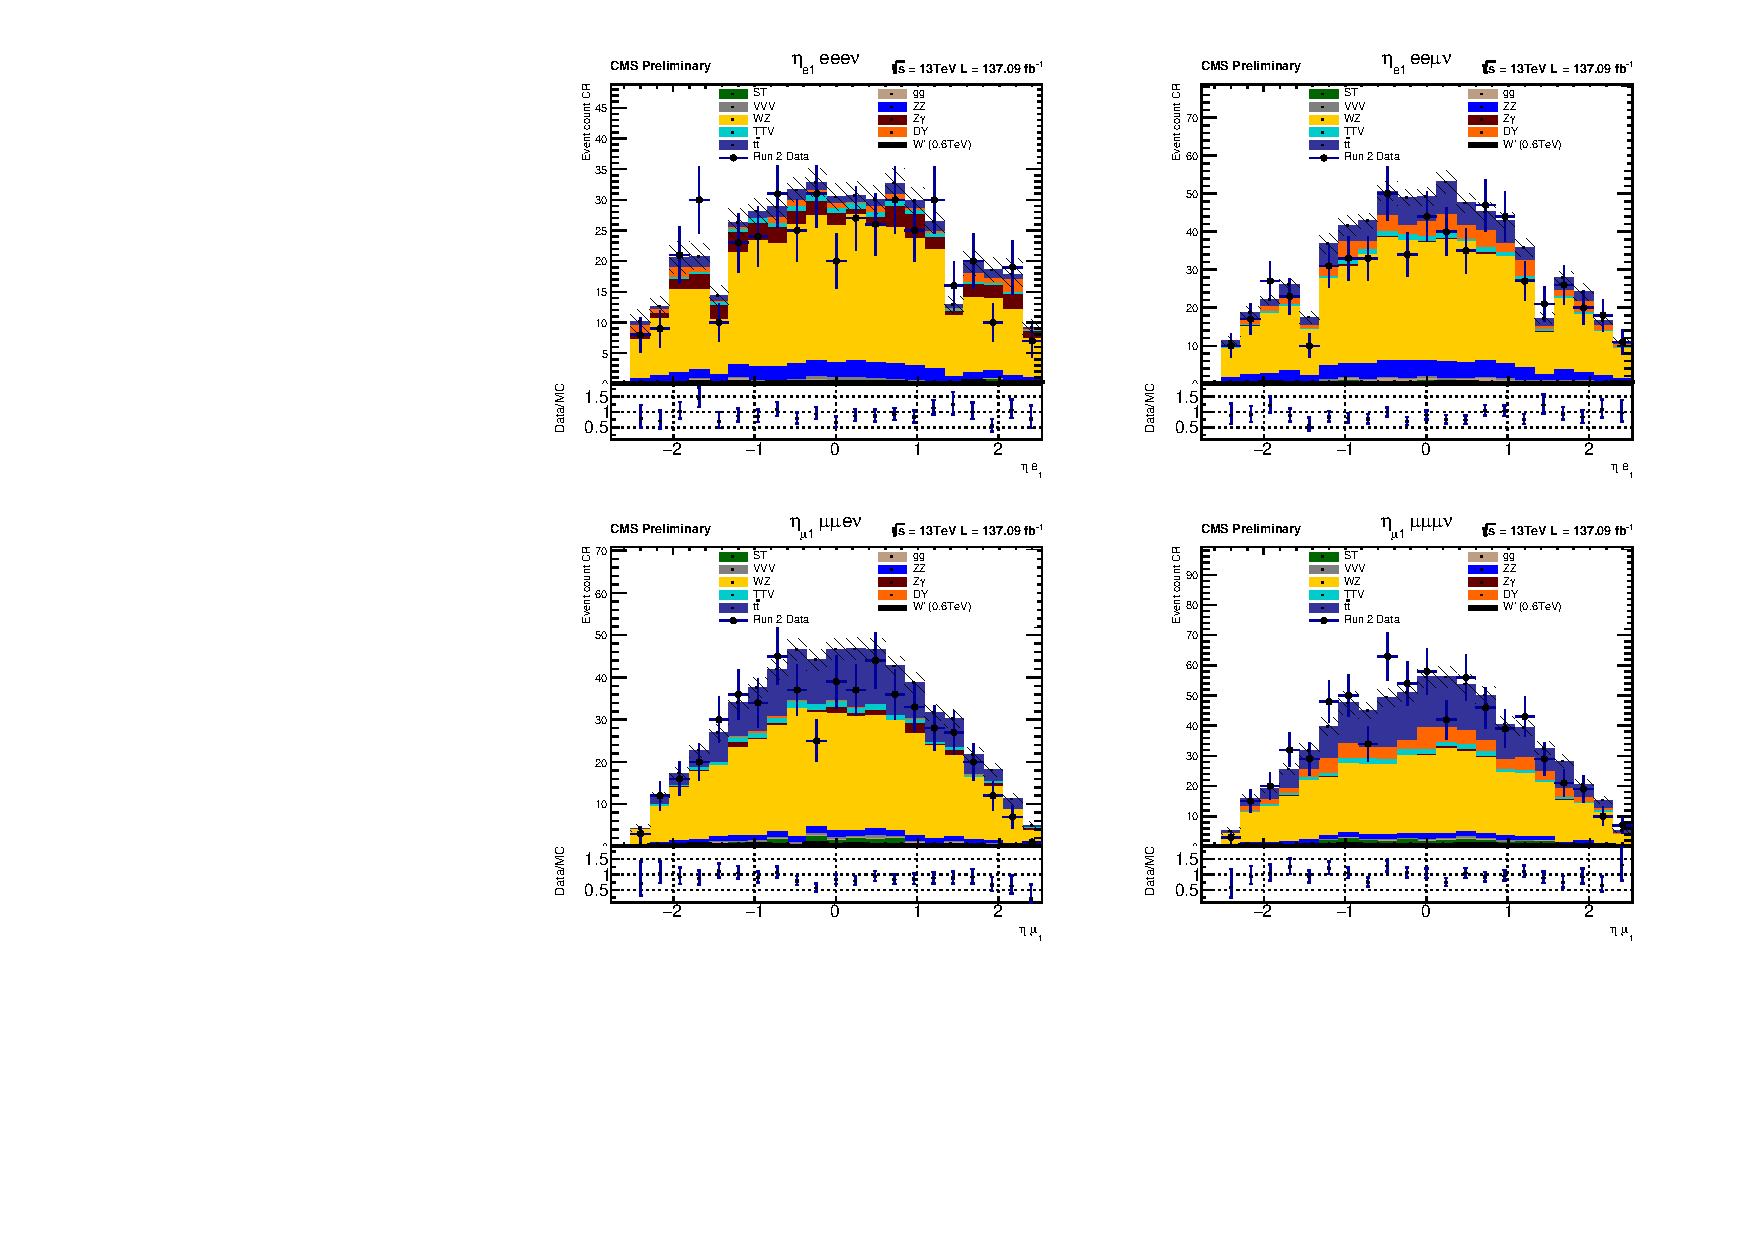
\includegraphics[width=\textwidth]{fig/Run2/KFactorIncluded_HEtal1_CR1_A_Run2_HERun2_M600.pdf}
  \caption{Leading lepton $\eta$ distributions for each final
    signature as seen in the $dr_{l_{1}l_{2}} > 1.5$ control region.
    Top left: $Z(\rightarrow e+e)W(\rightarrow e+\nu)$
    Top right: $Z(\rightarrow e+e)W(\rightarrow \mu+\nu)$
    Bottom left: $Z(\rightarrow \mu+\mu)W(\rightarrow e+\nu)$
    Bottom right: $Z(\rightarrow \mu+\mu)W(\rightarrow \mu+\nu)$}
  \label{fig:CR1_Run2_HEtal1}
\end{figure}

\begin{figure}[tph]
  \centering
  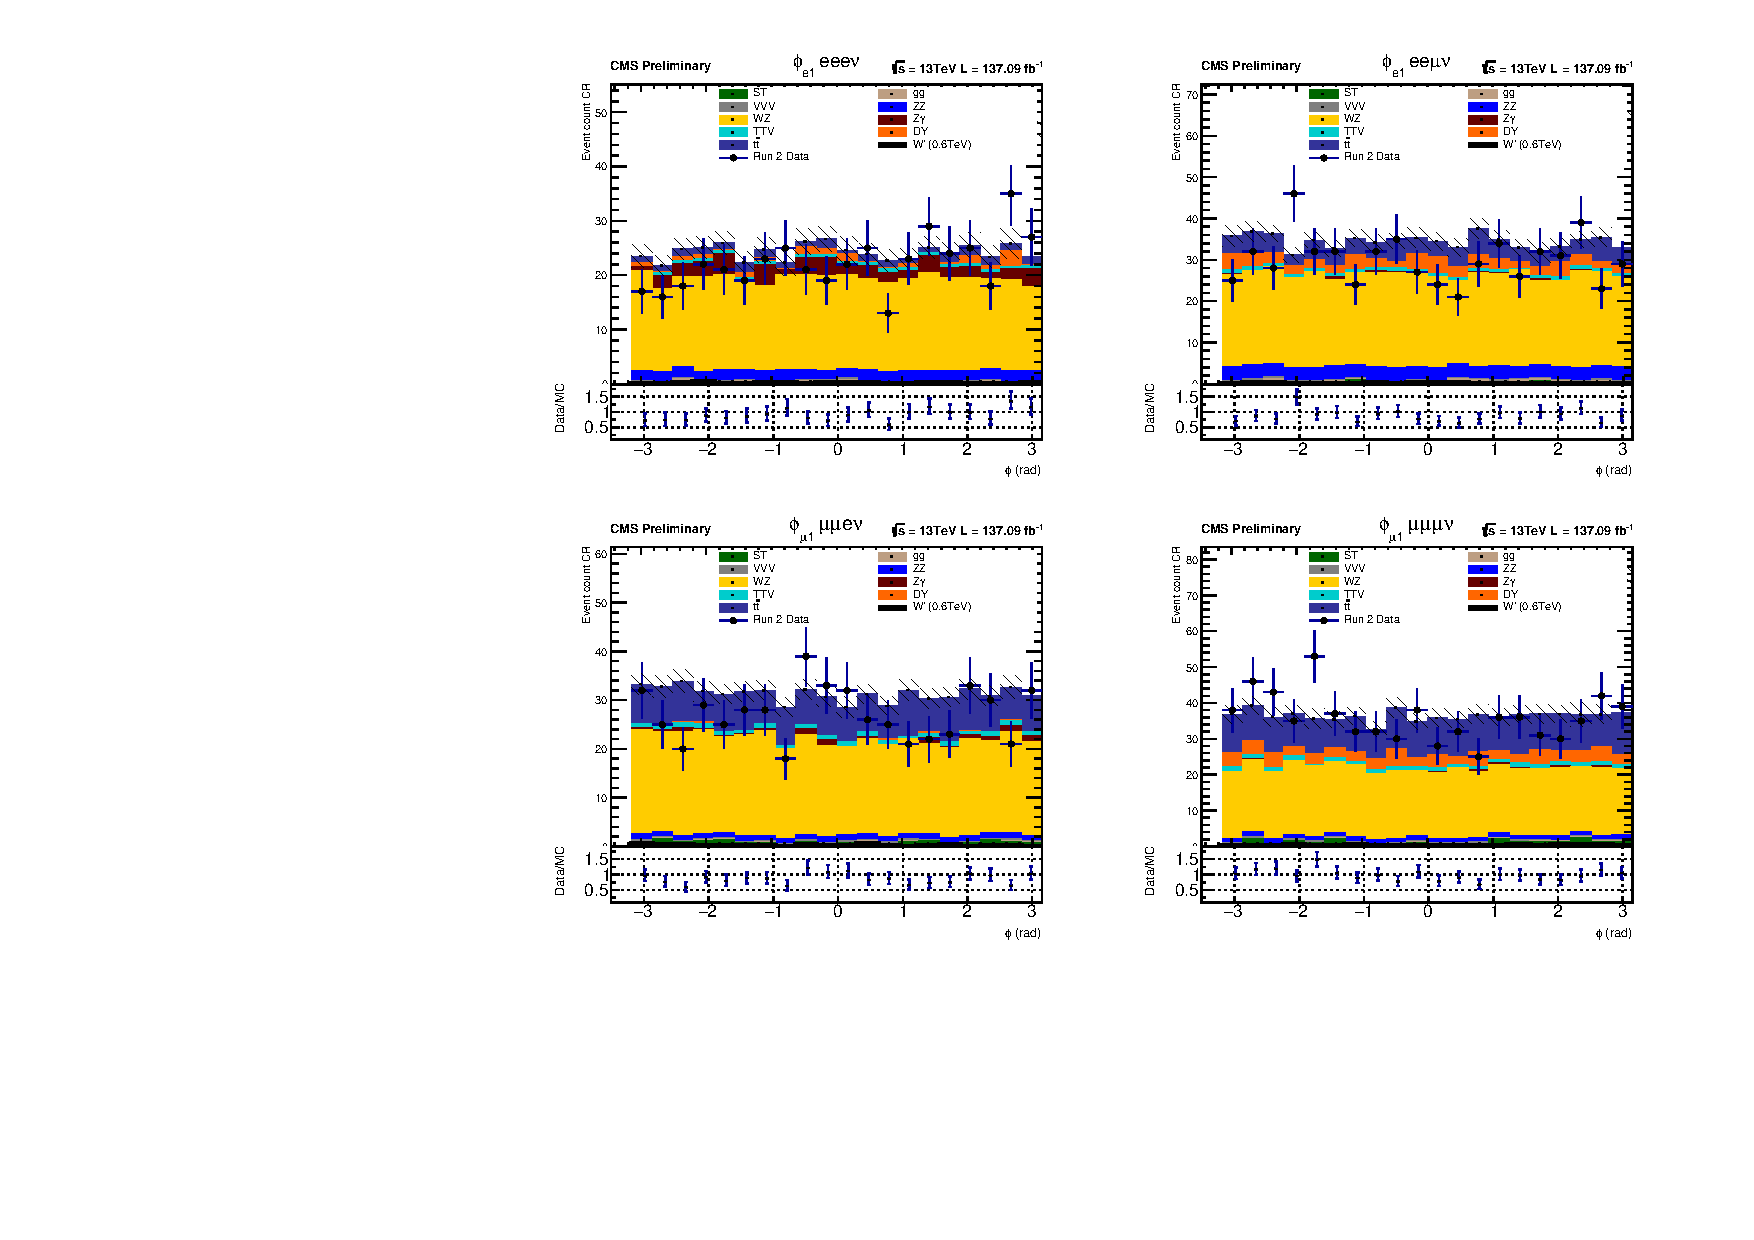
\includegraphics[width=\textwidth]{fig/Run2/KFactorIncluded_HPhil1_CR1_A_Run2_HPRun2_M600.pdf}
  \caption{Leading lepton $phi$ distributions for each final
    signature as seen in the $dr_{l_{1}l_{2}} > 1.5$ control region.
    Top left: $Z(\rightarrow e+e)W(\rightarrow e+\nu)$
    Top right: $Z(\rightarrow e+e)W(\rightarrow \mu+\nu)$
    Bottom left: $Z(\rightarrow \mu+\mu)W(\rightarrow e+\nu)$
    Bottom right: $Z(\rightarrow \mu+\mu)W(\rightarrow \mu+\nu)$}
  \label{fig:CR1_Run2_HPhil1}
\end{figure}

\begin{figure}[tph]
  \centering
  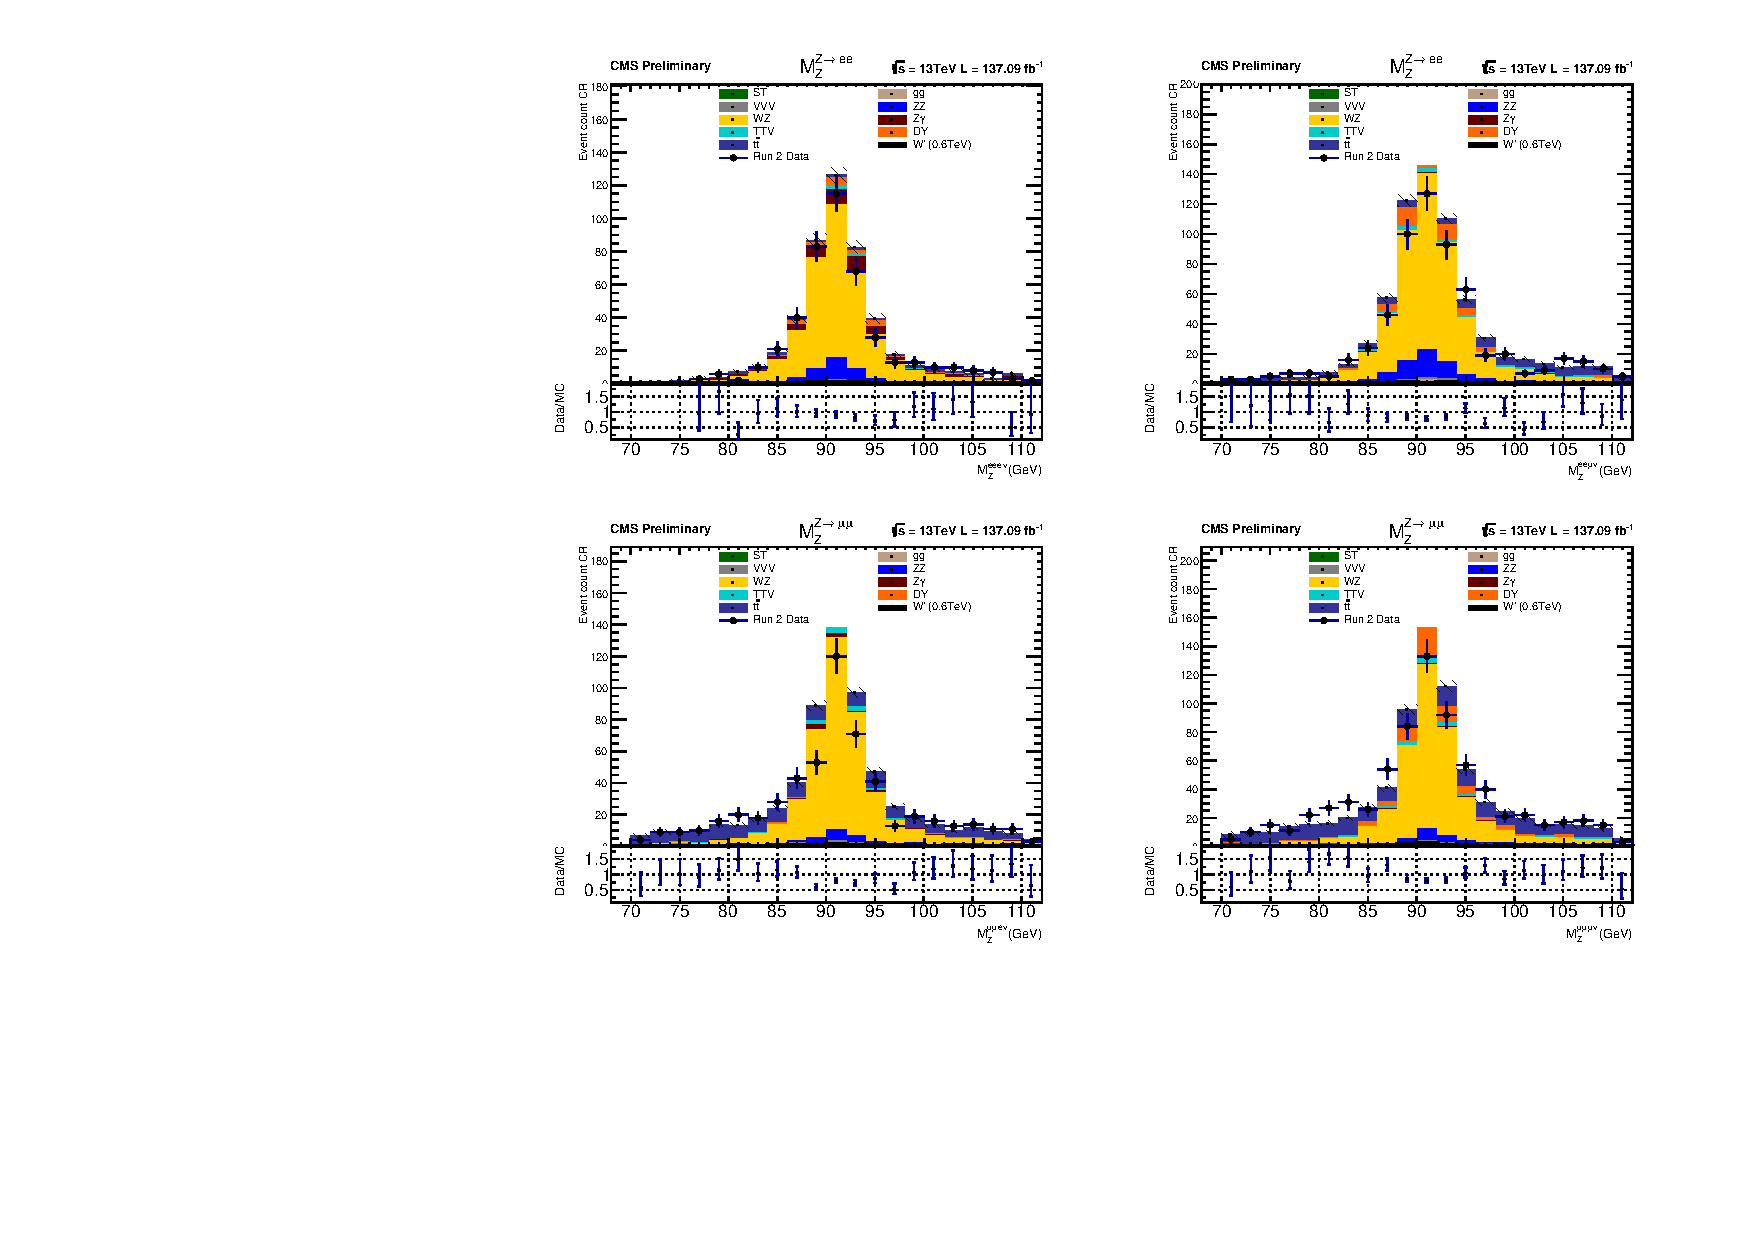
\includegraphics[width=\textwidth]{fig/Run2/KFactorIncluded_HMassZ_CR1_A_Run2_HMRun2_M600.pdf}
  \caption{$M_{Z}$ distributions of $Z\rightarrow\ell\ell$ candidates for each final
    signature as seen in the $dr_{l_{1}l_{2}} > 1.5$ control region.
    Top left: $Z(\rightarrow e+e)W(\rightarrow e+\nu)$
    Top right: $Z(\rightarrow e+e)W(\rightarrow \mu+\nu)$
    Bottom left: $Z(\rightarrow \mu+\mu)W(\rightarrow e+\nu)$
    Bottom right: $Z(\rightarrow \mu+\mu)W(\rightarrow \mu+\nu)$}
  \label{fig:CR1_Run2_HMassZ}
\end{figure}

\begin{figure}[tph]
  \centering
  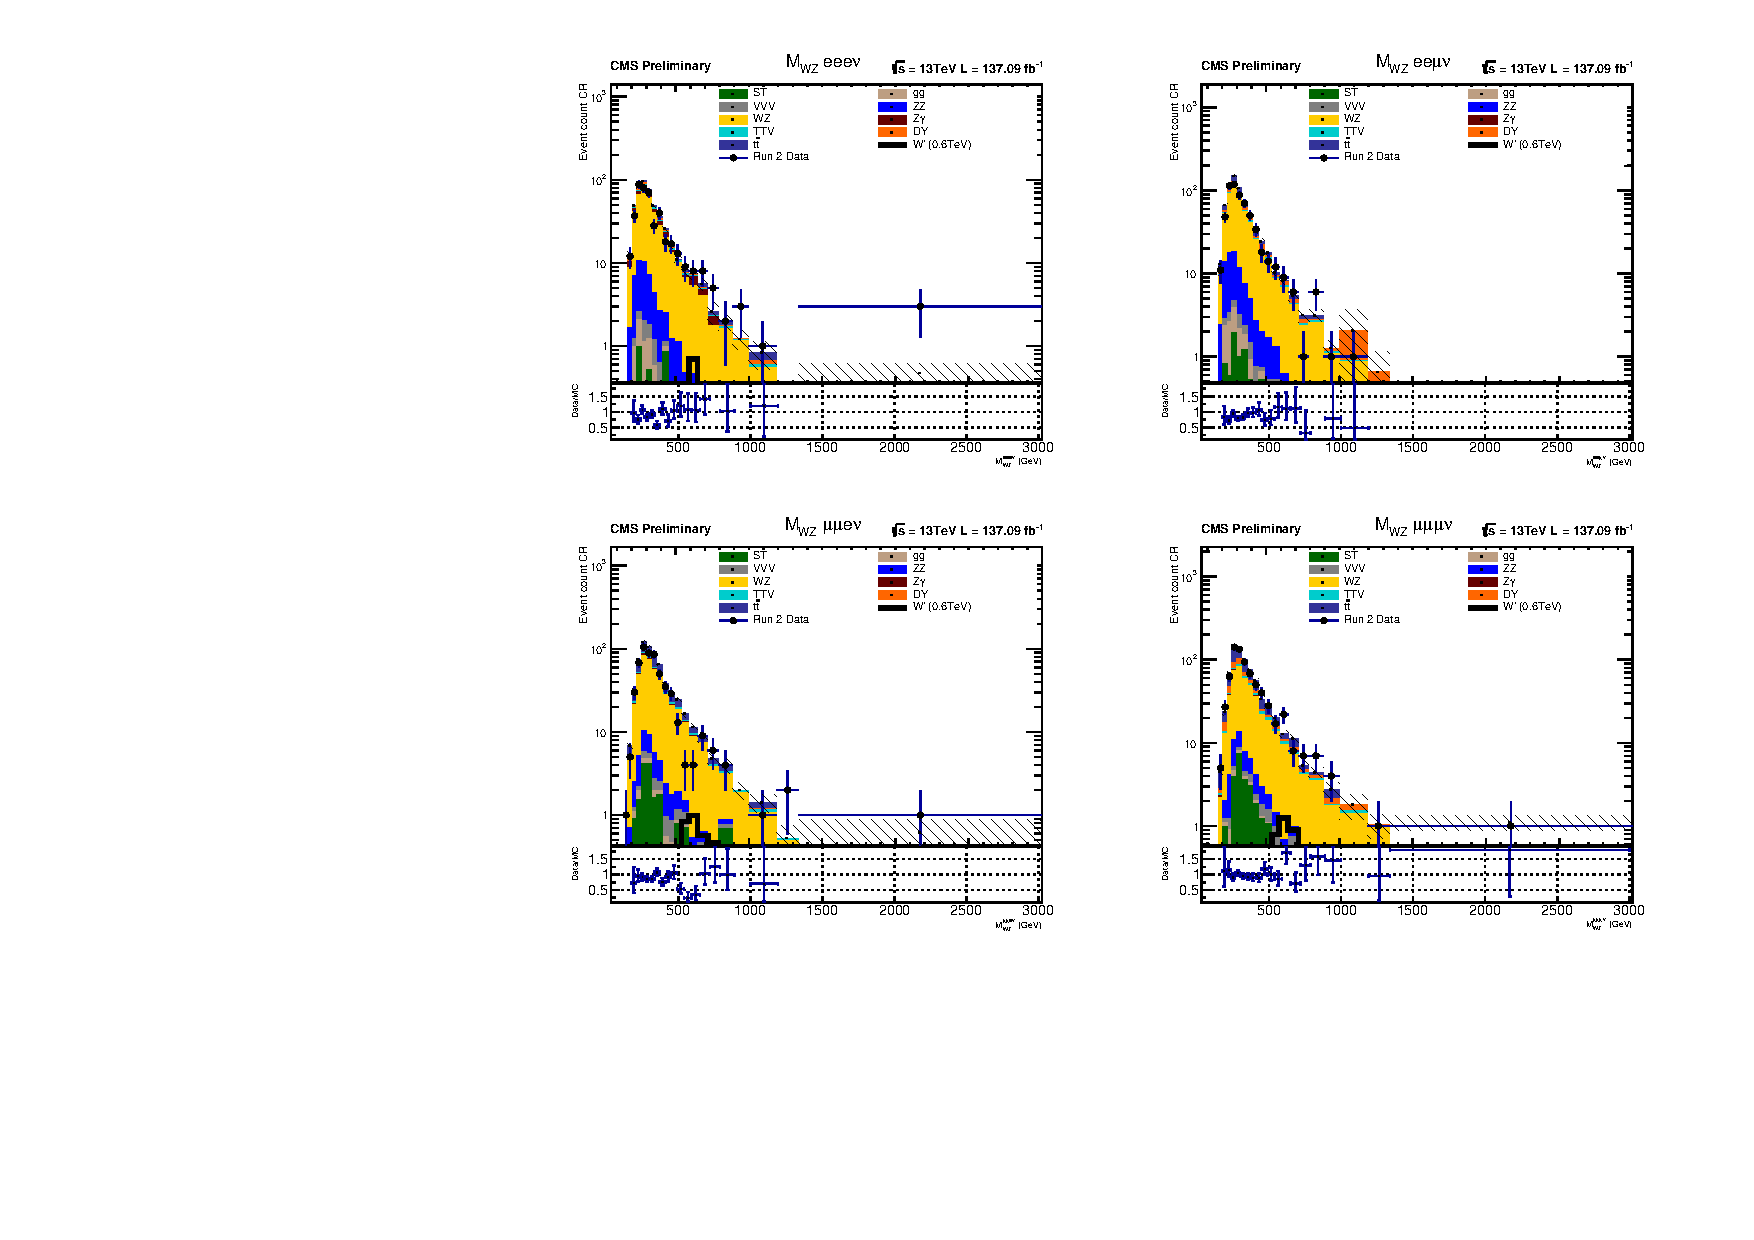
\includegraphics[width=\textwidth]{fig/Run2/Rebining_HMassWZ_CR1_A_Run2_HRun2_M600.pdf}
  \caption{The $WZ$ invariant mass after the $WZ$ candidate selection for each final
    signature as seen in the $dr_{l_{1}l_{2}} > 1.5$ control region.
    Top left: $Z(\rightarrow e+e)W(\rightarrow e+\nu)$
    Top right: $Z(\rightarrow e+e)W(\rightarrow \mu+\nu)$
    Bottom left: $Z(\rightarrow \mu+\mu)W(\rightarrow e+\nu)$
    Bottom right: $Z(\rightarrow \mu+\mu)W(\rightarrow \mu+\nu)$}
  \label{fig:CR1_Run2_HMassWZ}
\end{figure}

\begin{figure}[tph]
  \centering
  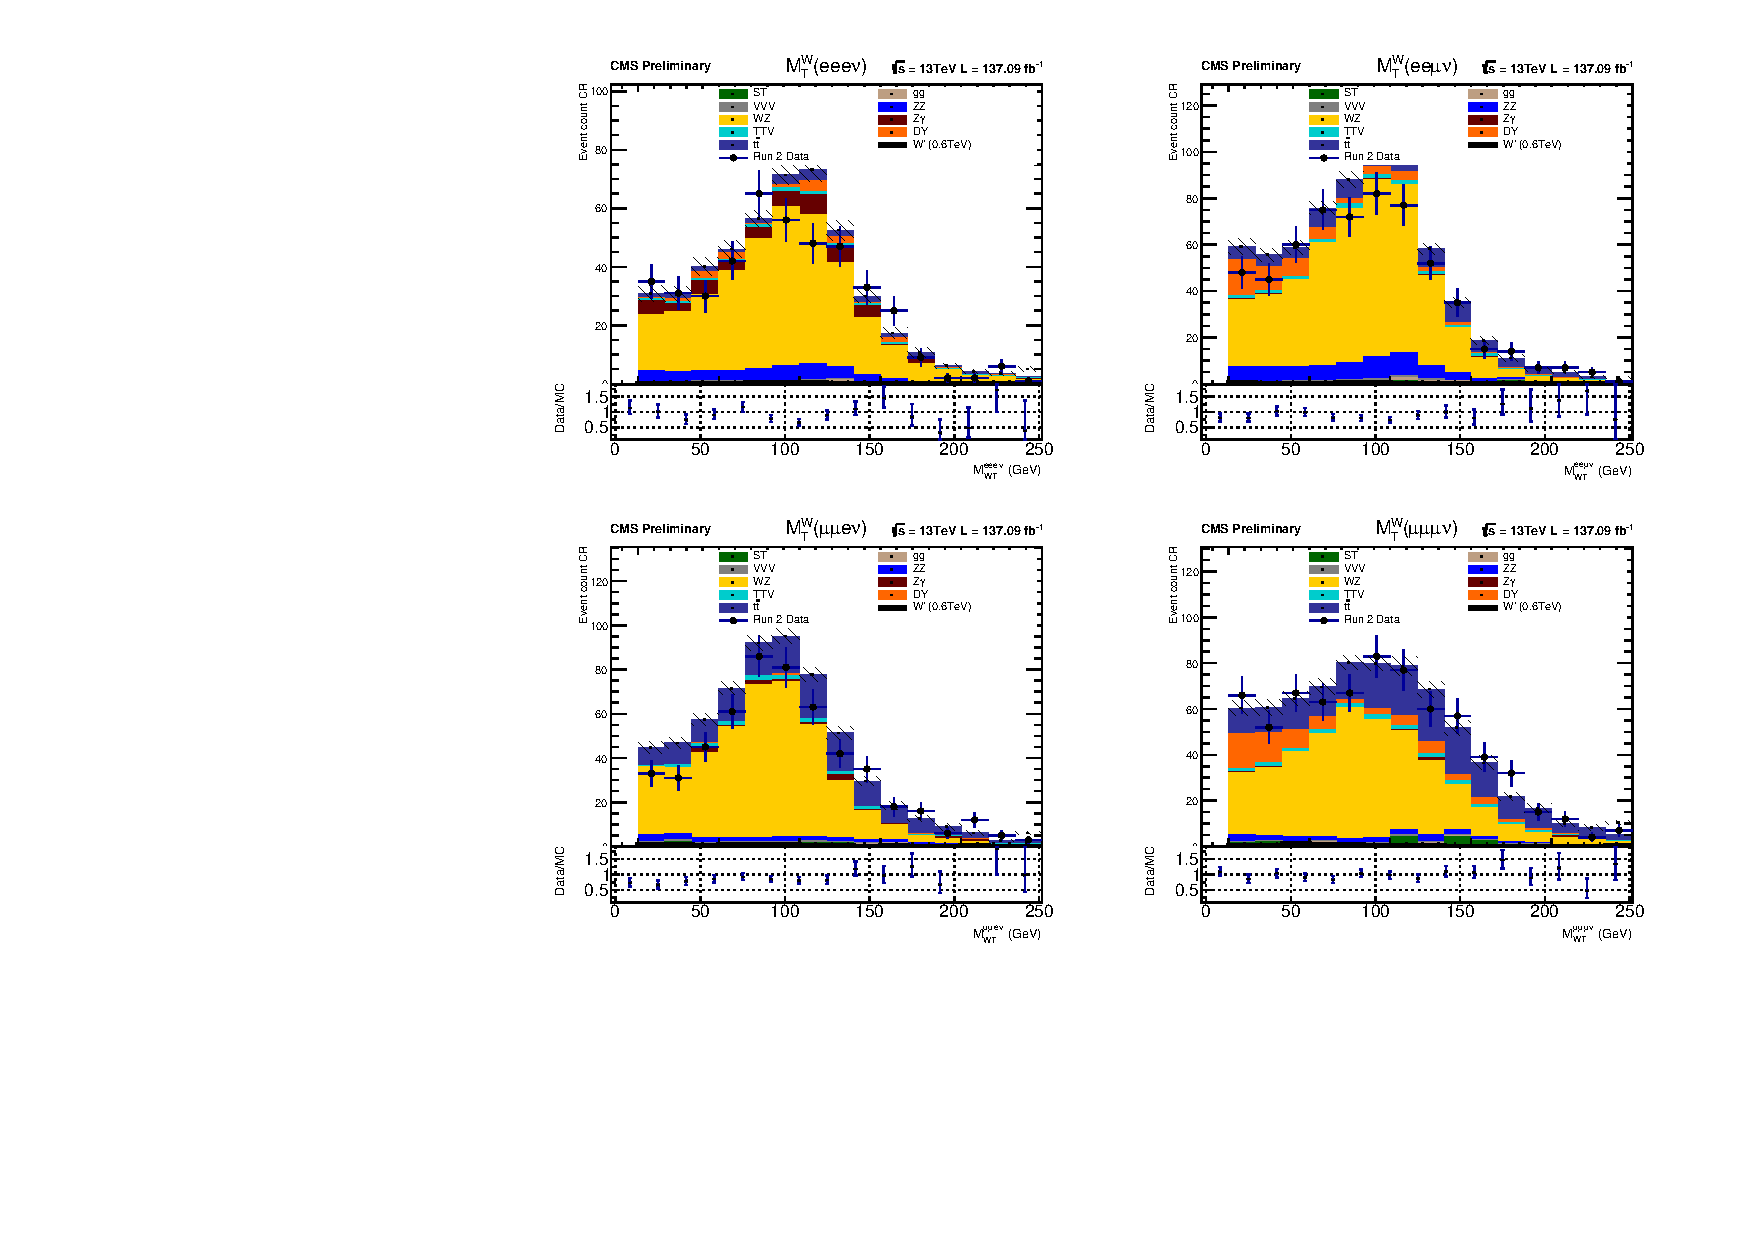
\includegraphics[width=\textwidth]{fig/Run2/KFactorIncluded_HMassTW_CR1_A_Run2_HRun2_M600.pdf}
  \caption{The transverse mass distribution for the $W$ candidate for each final
    signature as seen in the $dr_{l_{1}l_{2}} > 1.5$ control region.
    Top left: $Z(\rightarrow e+e)W(\rightarrow e+\nu)$
    Top right: $Z(\rightarrow e+e)W(\rightarrow \mu+\nu)$
    Bottom left: $Z(\rightarrow \mu+\mu)W(\rightarrow e+\nu)$
    Bottom right: $Z(\rightarrow \mu+\mu)W(\rightarrow \mu+\nu)$}
  \label{fig:CR1_Run2_HMassTW}
\end{figure}

The $\eta$, $\phi$, $P_{T}$ distributions for the leading lepton en each category
are shown in figures \ref{fig:CR1_Run2_HEtal1}, \ref{fig:CR1_Run2_HPhil1}, and
\ref{fig:CR1_Run2_HPtl1}, as well as composite distributions like the mass of the
reconstructed Z candidate (Figure \ref{fig:CR1_Run2_HMassZ}), the $W$ boson transverse mass
(Figure \ref{fig:CR1_Run2_HMassTW}) and the discriminant variable: the mass for the
reconstructed diboson system (Figure \ref{fig:CR1_Run2_HMassWZ}) show a good data/MC
agreement in the control region.


\begin{table}
  \caption{Background Yields per
    channel on Control Region}
 \begin{center}
 \begin{tabular}{cccccc}\hline\hline
Sample & $eee\nu$ & $ee\mu\nu$ & $\mu\mu e\nu$ & $\mu\mu\mu\nu$ & Total \\
DY & 15.87 & 53.38 & 2.09 & 65.86 & 137.19 \\
ST & 3.14 & 7.46 & 17.89 & 25.60 & 54.09 \\
TTV & 11.23 & 16.91 & 18.10 & 22.27 & 68.51 \\
VVV & 4.29 & 5.67 & 5.66 & 5.85 & 21.46 \\
WZ & 337.97 & 443.60 & 395.82 & 380.23 & 1,557.63 \\
$Z\gamma$ & 43.00 & 1.94 & 9.89 & 2.09 & 56.91 \\
ZZ & 38.58 & 65.07 & 22.31 & 25.54 & 151.50 \\
gg & 4.84 & 8.53 & 2.74 & 2.59 & 18.70 \\ \hline
Total Background & 458.91 & 602.57 & 474.50 & 530.03 & 2,066.01 \\ \hline
Total Data & 442.00 & 601.00 & 542.00 & 718.00 & 2,303.00 \\ \hline
 \end{tabular}
 \end{center}
 \label{tab:BackgroundYieldsCR}
\end{table}

\begin{table}
  \caption{Background Yields per
    channel on Signal Region}
 \begin{center}
 \begin{tabular}{cccccc}\hline\hline
Sample & $eee\nu$ & $ee\mu\nu$ & $\mu\mu e\nu$ & $\mu\mu\mu\nu$ & Total \\
DY & 9.88 & 225.94 & 225.94 & 232.50 & 694.26 \\
ST & 0.84 & 6.23 & 6.23 & 19.66 & 32.96 \\
TTV & 10.64 & 47.18 & 47.18 & 59.60 & 164.60 \\
VVV & 4.30 & 12.34 & 12.34 & 16.29 & 45.27 \\
WZ & 183.82 & 571.75 & 571.75 & 643.67 & 1,970.99 \\
$Z\gamma$ & 17.71 & 10.01 & 10.01 & 7.41 & 45.13 \\
ZZ & 18.74 & 47.29 & 47.29 & 30.69 & 144.01 \\
gg & 2.12 & 6.36 & 6.36 & 2.16 & 16.99 \\ \hline
Total Background & 248.04 & 927.11 & 927.11 & 1,011.96 & 3,114.22 \\ \hline
 \end{tabular}
 \end{center}
 \label{tab:BackgroundYieldsSR}
\end{table}


\section{Uncertainties}

\section{Corrections on MC}

\begin{figure}[tph]
  \centering
        \subfigure[Electron Loose ID]{\includegraphics[width=.28\textwidth]{fig/2016Electron_LooseID.pdf}}
        \subfigure[Muon GlobalHighPtId]{\includegraphics[width=.28\textwidth]{fig/2016Muon_GlobalHighPtID.pdf}}
        \subfigure[Muon TrkHighPtId]{\includegraphics[width=.28\textwidth]{fig/2016Muon_TrkHighPtID.pdf}}
  \caption{SF for different lepton ids}
  \label{fig:leptonidsf}
\end{figure}




\section{Results}


\section{Results}

Exclusion limits on the production cross section $\sigma$ are computed by
comparing the number of observed events with the number of expected signal
and background events. 


\section{Muon Momentum Resolution}

by travelling in Iron, High-Pt muons ($P_{t}>200GeV$) suffer from high energy
loss due to radiative processes. The transverse momentum measurement relays on
sagita ($s \propto 1/Pt$) which is associated with the number of hits found on
the Tracker and the Muon subsystems. As the number of hits is lower on the so called
tracker muons, i.e muons that were reconstructed from hits in the tracker and the
first station of the muon sistem, a study is needed to determine
the resolution of this Pt measurement for tracker-HighPt ID muons.

From MC simulations it is possible to access the true momenta of the muons and
a comparison with the reconstructed momentum can be given in terms of the
residual momentum:

\begin{equation}
  \frac{P_{GEN}}{P_{RECO}} - 1 = \frac{\dfrac{1}{P_{RECO}}-\dfrac{1}{P_{GEN}}}{\dfrac{1}{P_{RECO}}}
\end{equation}

The resolution can be extracted by fitting the event profile with a
Double-Sided Crystal Ball distribution wich consists of three diferent regions:
a gaussian center described by a mean $\mu$ and standard deviation $\sigma$ with two
exponential tails modelling the effects of radiative processes in the detector.
The two tails are controlled by four parameters, $n_L$ and $\alpha_L$ for the
left tail and $n_R$ and $\alpha_R$ for the right tail. $\alpha$ describes how
far away (as a factor of $sigma$) from the gaussian mean the exponential decay
intersects the guassian core, while $n$ controls the growth (decay) of the
left (right) exponential tail.


\begin{sidewaystable}[htb]
\begin{center}
  \caption{Montecarlo Samples used to study the Muon Momentum Resolution}
\footnotesize
\begin{tabular}{|l|l|l|}
\hline
Year & Sample & XSec [pb] \\ \hline
\hline
2016 & ZToMuMu\_NNPDF30\_13TeV-powheg\_M\_50\_120 & 2.116e+03\\
&ZToMuMu\_NNPDF30\_13TeV-powheg\_M\_120\_200 & 2.058e+01\\
&ZToMuMu\_NNPDF30\_13TeV-powheg\_M\_200\_400 & 2.890e+00\\
&ZToMuMu\_NNPDF30\_13TeV-powheg\_M\_400\_800 & 2.515e-01\\
&ZToMuMu\_NNPDF30\_13TeV-powheg\_M\_800\_1400 & 1.709e-02\\
&ZToMuMu\_NNPDF30\_13TeV-powheg\_M\_1400\_2300 & 1.370e-03\\
&ZToMuMu\_NNPDF30\_13TeV-powheg\_M\_2300\_3500 & 8.282e-05\\
&ZToMuMu\_NNPDF30\_13TeV-powheg\_M\_3500\_4500 & 3.414e-06\\
&ZToMuMu\_NNPDF30\_13TeV-powheg\_M\_4500\_6000 & 3.650e-07\\
&ZToMuMu\_NNPDF30\_13TeV-powheg\_M\_6000\_Inf & 2.526e-08\\
\hline
2017 & ZToMuMu\_NNPDF31\_TuneCP5\_13TeV-powheg-pythia8\_M\_50\_120 & 2.116e+03\\
&ZToMuMu\_NNPDF31\_TuneCP5\_13TeV-powheg-pythia8\_M\_120\_200 & 2.058e+01\\
&ZToMuMu\_NNPDF31\_TuneCP5\_13TeV-powheg-pythia8\_M\_200\_400 & 2.890e+00\\
&ZToMuMu\_NNPDF31\_TuneCP5\_13TeV-powheg-pythia8\_M\_400\_800 & 2.515e-01\\
&ZToMuMu\_NNPDF31\_TuneCP5\_13TeV-powheg-pythia8\_M\_800\_1400 & 1.709e-02\\
&ZToMuMu\_NNPDF31\_TuneCP5\_13TeV-powheg-pythia8\_M\_1400\_2300 & 1.370e-03\\
&ZToMuMu\_NNPDF31\_TuneCP5\_13TeV-powheg-pythia8\_M\_2300\_3500 & 8.282e-05\\
&ZToMuMu\_NNPDF31\_TuneCP5\_13TeV-powheg-pythia8\_M\_3500\_4500 & 3.414e-06\\
&ZToMuMu\_NNPDF31\_TuneCP5\_13TeV-powheg-pythia8\_M\_4500\_6000 & 3.650e-07\\
&ZToMuMu\_NNPDF31\_TuneCP5\_13TeV-powheg-pythia8\_M\_6000\_Inf & 2.526e-08\\
\hline
2018 & ZToMuMu\_NNPDF31\_TuneCP5\_13TeV-powheg-pythia8\_M\_50\_120 & 2.116e+03\\
&ZToMuMu\_NNPDF31\_TuneCP5\_13TeV-powheg-pythia8\_M\_120\_200 & 2.058e+01\\
&ZToMuMu\_NNPDF31\_TuneCP5\_13TeV-powheg-pythia8\_M\_200\_400 & 2.890e+00\\
&ZToMuMu\_NNPDF31\_TuneCP5\_13TeV-powheg-pythia8\_M\_400\_800 & 2.515e-01\\
&ZToMuMu\_NNPDF31\_TuneCP5\_13TeV-powheg-pythia8\_M\_800\_1400 & 1.709e-02\\
&ZToMuMu\_NNPDF31\_TuneCP5\_13TeV-powheg-pythia8\_M\_1400\_2300 & 1.370e-03\\
&ZToMuMu\_NNPDF31\_TuneCP5\_13TeV-powheg-pythia8\_M\_2300\_3500 & 8.282e-05\\
&ZToMuMu\_NNPDF31\_TuneCP5\_13TeV-powheg-pythia8\_M\_3500\_4500 & 3.414e-06\\
&ZToMuMu\_NNPDF31\_TuneCP5\_13TeV-powheg-pythia8\_M\_4500\_6000 & 3.650e-07\\
&ZToMuMu\_NNPDF31\_TuneCP5\_13TeV-powheg-pythia8\_M\_6000\_Inf & 2.526e-08\\
\hline
\end{tabular}
\label{tab:MomentumResolutionSamples}
\end{center}
\end{sidewaystable}

These studies were performed by simulating the standard model Z boson production
decaying to a pair of Muons ($Z\rightarrow\mu\mu$) the complete list of samples is
provided on table \ref{tab:MomentumResolutionSamples}
Z-Mass binned samples were used in order to increase the number of available
statistics in a wide range of transverse momentum, specially on the High-Pt sector.

\begin{figure}[tph]
  \centering
  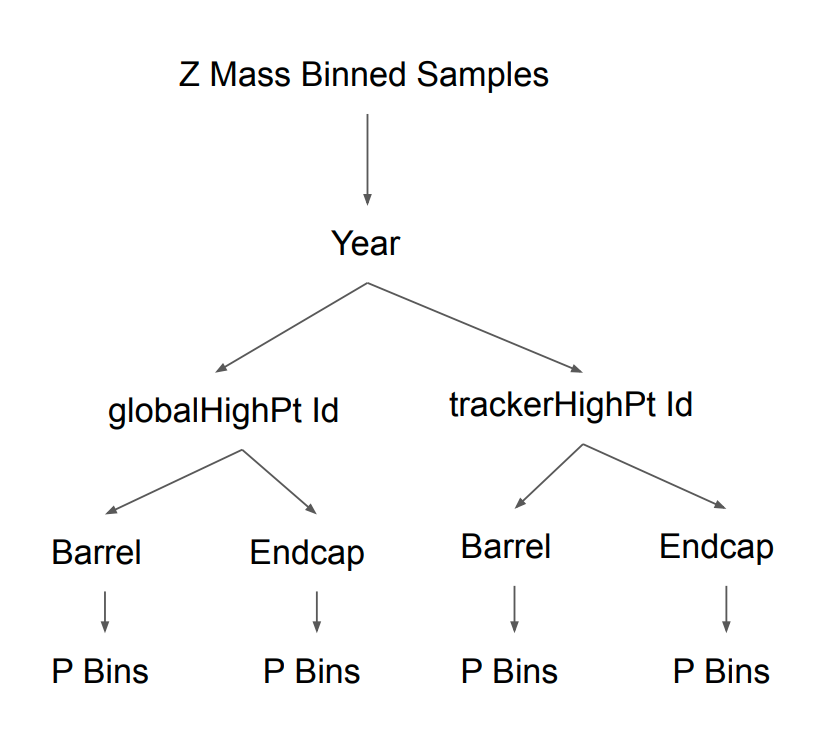
\includegraphics[width=.5\textwidth]{fig/MomentumResolution/MomentumResolutionBins.png}
  \caption{Signal efficiency for individual and combined High Level Triggers for Run II}
  \label{fig:MomentumResolutionBins}
\end{figure}

A counting experiment following the trigger and muon selection described on
section %\ref{}%
collects the momentum resolution for each indivual Muon which is then classified
on different bins depending on its ID, either global or tracker High-Pt; the $\eta$
region in the Muon detector, i.e the barrel ($\lvert eta\lvert< 1.2$) or
the endcap ($1.2 < \lvert eta \lvert < 2.4$); and its transverse momentum range
(see figure \ref{fig:MomentumResolutionBins}).


\begin{figure}[tph]
  \centering
  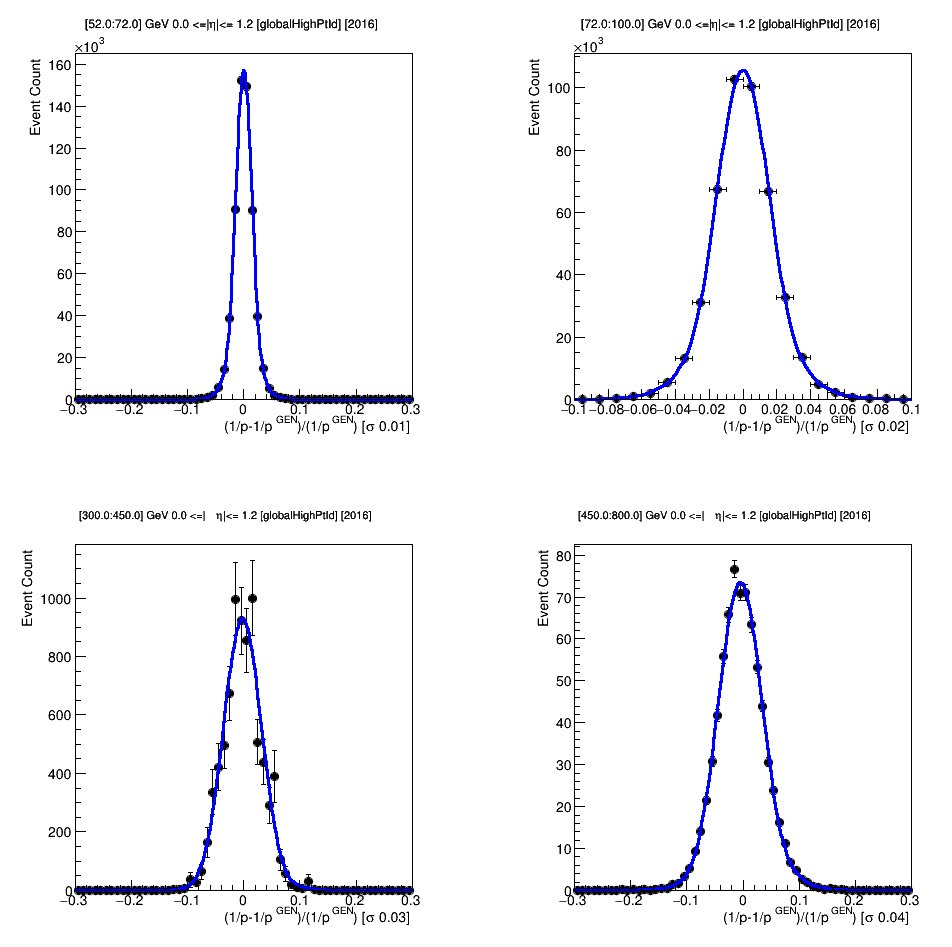
\includegraphics[width=.7\textwidth]{fig/MomentumResolution/DSCB_Example.png}
  \caption{
    The Double-Sided Crystall Ball fit is shown as the blue solid line,
    the number of events as counted from MC samples are shown in black markers for
    the momentum resolution. The example shows the 2016 samples for muons labeled
    as globalHigh-Pt, seen in the barrel of the muon system. Different momentum
    ranges are shown, the
    top-left figure shows muons with momentum in the range $[52:72]~GeV$,
    the top-right figure $[72:100]~GeV$, bottom-left $[300:450]~GeV$,
    bottom-right $[450:800]~GeV$. The value for the width $\sigma$ for the DSCB
    distribution is shown on the horizontal axis and it shows evidence of how
    the resolution increases as the momentum range gets higher.
  }
  \label{fig:DSCB_Fit_Example}
\end{figure}

The distribution is then fitted by using a Double-Sided Crystall Ball (DSCB)
(\verb|RooCrystalBall| in \verb|RooFit|) which is a distribution defined
by parts, with a range-limited gaussian form around its mean with two
exponential tails which help model the nature of radiative processes occurring in
the detector. The width of the gaussian portion of the DSCB provides the
resolution (as a percentage) while the mean accounts for any bias present on the
momentum measurements. An example of the fit is shown in \ref{fig:DSCB_Fit_Example}

% Events with low statistics in bins are discarded

\subsection{Z-Mass Resolution}

\begin{sidewaystable}[htb]
\begin{center}
  \caption{Montecarlo Samples for Z Mass Resolution studies}
\footnotesize
\begin{tabular}{|l|l|l|}
\hline
Year & Sample & XSec [pb] \\ \hline
\hline
2016 & DYJetsToMuMu\_M-50\_Zpt-150toInf\_TuneCP5\_13TeV-madgraphMLM\_pdfwgt\_F-pythia8 & 6.178e+00\\
\hline
2017 & DYJetsToMuMu\_M-50\_Zpt-150toInf\_TuneCP5\_13TeV-madgraphMLM\_pdfwgt\_F-pythia8 & 6.182e+00\\
\hline
2018 & DYJetsToMuMu\_M-50\_Zpt-150toInf\_TuneCP5\_13TeV-madgraphMLM\_pdfwgt\_F-pythia8 & 6.178e+00\\
\hline
\end{tabular}
\label{tab:ZMassResolutionSamples}
\end{center}
\end{sidewaystable}



%% **DO NOT REMOVE BIBLIOGRAPHY**
\bibliography{auto_generated}
%% examples of appendices.
%\clearpage
%\appendix
%\section{Appendix name}
%%% DO NOT ADD \end{document}!

